\documentclass[10pt]{article}
\usepackage[utf8]{inputenc}
\usepackage[italian]{babel}
\usepackage{multicol}
\usepackage[a4paper, total={18cm, 25cm}]{geometry}
\usepackage{listings}
\usepackage{graphicx}
\graphicspath{ {./img/} }
\usepackage{color}

\begin{document}
\title{Reti di Calcolatori e Laboratorio}
\author{Federico Matteoni}
\date{ }
\renewcommand*\contentsname{Indice}
\definecolor{pblue}{rgb}{0.13,0.13,1}
\definecolor{pgreen}{rgb}{0,0.5,0}
\definecolor{pred}{rgb}{0.9,0,0}
\definecolor{pgrey}{rgb}{0.46,0.45,0.48}
\lstset{
  language=Java,
  showspaces=false,
  showtabs=false,
  breaklines=true,
  showstringspaces=false,
  breakatwhitespace=true,
  commentstyle=\color{pgreen},
  keywordstyle=\color{pblue},
  stringstyle=\color{pred},
  basicstyle=\small\ttfamily
}

\maketitle
\begin{multicols}{2}
\tableofcontents
\end{multicols}
\pagebreak
\section{Introduzione}
Appunti del corso di \textbf{Reti di Calcolatori} presi a lezione da \textbf{Federico Matteoni}.\\\\
Prof.: \textbf{Federica Paganelli}, federica.paganelli@unipi.it\\
\begin{list}{-}{Riferimenti web:}
\item \emph{elearning.di.unipi.it/enrol/index.php?id=169}\\Password: \textbf{RETI2019}
\end{list}
Esame: scritto (o compitini), discussione orale facoltativa + progetto con discussione (progetto + teoria di laboratorio, progetto da consegnare 7gg prima della discussione)\\
\begin{list}{-}{Libri e materiale didattico:}
\item Slide su eLearning
\item IETF RFC\\tools.ietf.org/rfc\\www.ietf.org/rfc.html
\item "Computer Networks: A Top-Down Approach" B. A. Forouzan, F. Mosharraf, McGraw Hill
\end{list}
Ricevimento: stanza 355 DO, II piano

\begin{verbatim}
Immagini: Copyright 1996-2005 J.F Kurose and K.W. Ross
\end{verbatim}
\pagebreak
\section{Rete}
\paragraph{Definizione di rete} Interconnessione di dispositivi in grado di scambiarsi informazioni, come end system, router, switch e modem.\\
\begin{list}{}{Gli end system possono essere di due tipi:}
\item \textbf{Host}: una macchina, in genere di proprietà degli utenti, \textbf{dedicata ad eseguire applicazioni}. Esempi: desktop, portatile, smartphone, tablet\ldots
\item \textbf{Server}: una macchina, tipicamente con elevate prestazioni, destinata ad eseguire programmi che \textbf{forniscono servizi} a diverse applicazioni utente. Esempi: posta elettronica, web, \ldots
\end{list}
\textbf{Con il termine host si può anche indicare un server}.

\subsection{Tipi di Rete}
\paragraph{Local Area Network} Una \textbf{LAN è una rete di area geografica limitata}: un ufficio, una casa ecc.. I dispositivi comunicano attraverso una determinata tecnologica: switch, BUS, HUB ecc..\\
In una rete locale tipicamente una serie di host comunicano tra loro attraverso, ad esempio, uno switch centrale.
\paragraph{Wide Area Network} Alcuni esempi:\\
\begin{multicols}{2}
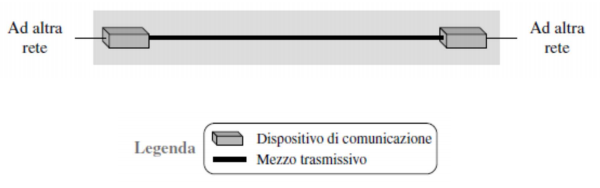
\includegraphics[scale=0.5]{wan1.png}\\
\columnbreak
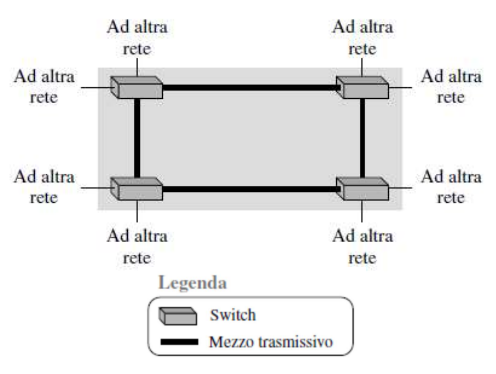
\includegraphics[scale=0.5]{wan2.png}\\
\end{multicols}

\subsection{Internetwork}
Una \textbf{internetwork} si crea quando si \textbf{interconnettono diverse reti}.
Alcuni esempi:\\
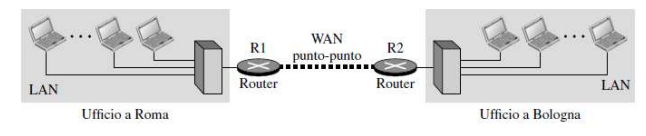
\includegraphics[scale=1]{internetwork1.png}\\
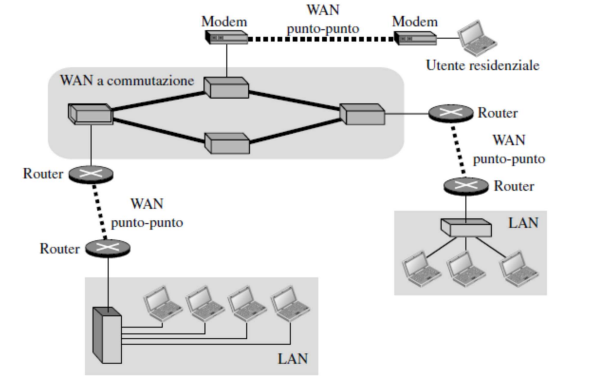
\includegraphics[scale=0.75]{internetwork2.png}\\

\subsection{Switching}
Una rete internet è formata dall'interconnesione di reti composte da link e dispositivi capaci di scambiarsi informazioni.
In particolare, i sistemi terminali comunicano tra di loro per mezzo di dispositivi come switch, router ecc. che si trovano nel percorso tra i sistemi sorgente e destinazione.
\paragraph{Switched Network} Reti a commutazione di circuito, tipico delle vecchie reti telefoniche\\
Le risorse sono riservate end-to-end per una connessione. Le risorse di rete (es. bandwidth) vengono suddivise in pezzi, e ciascun pezzo è allocato ai vari collegamenti. Le risorse rimangono inattive se non vengono utilizzate, cioè \textbf{non c'è condivisione}. L'allocazione della rete rende necessario un setup della comunicazione.\\A tutti gli effetti vi è un circuito dedicato per tutta la durata della connessione. Ciò è rende poco flessibile l'utilizzo delle risorse (\textbf{overprovisioning}).
\paragraph{Packet-Switched Network} Reti a commutazione di pacchetto, più moderno\\
Flusso di dati punto-punto suddiviso in pacchetti. I pacchetti degli utenti condividono le risorse di rete. Ciascun pacchetto utilizza completamente il canale.\\\textbf{Store and Forward}: il commutatore deve ricevere l'intero pacchetto prima di ritrasmetterlo in uscita.\\Le risorse vengono usate \textbf{a seconda delle necessità}. Vi è \textbf{contesa per le risorse}: la richiesta di risorse può eccedere la disponibilità e si può verificare \textbf{congestione} quando i pacchetti vengono accodati in attesa di utilizzare il collegamento. Si possono anche verificare perdite.
\section{Internet} L'internetwork più famosa ed utilizzata è \textbf{internet}, ed è composta da migliaia di reti interconnesse. \textbf{Ogni rete} connessa ad internet \textbf{deve utilizzare il protocollo IP} e rispettare certe convenzioni su nomi ed indirizzi. Si possono aggiungere nuove reti ad internet molto facilmente.
\paragraph{Dispositivi in internet} I \textbf{dispositivi} connessi ad internet possono essere host, end systems come PC, workstations, servers, pda, smartphones ecc\ldots\\
I \textbf{link di comunicazione} possono essere fibre ottiche, doppini telefonici, cavi coassiali, onde radio\ldots
Le \textbf{entità software} in internet possono essere:
\begin{list}{}{}
\item \textbf{Applicazioni} e processi
\item \textbf{Protocolli}: regolamentano la trasmissione e la ricezione di messaggi (TCP, IP, HTTP, FTP, PPP\ldots)
\item \textbf{Interfacce}
\item \textbf{Standard} di internet e del web: RFC (Request for Comments) e W3C.
\end{list}
\textbf{Internet è una visione dei servizi}. L'infrastruttura di comunicazione permette alle applicazioni distribuite di scambiare informazioni (WWW, e-mail, giochi, e-commerce, controllo remoto\ldots) e fornisce loro \textbf{servizi di comunicazione connectionless} (senza garanzia di consegna) o \textbf{connection-oriented} (dati garantiti in integrità, completezza ed ordine).
\subsection{Enti Ufficiali} L'\textbf{Internet Engineering Task Force} (IETF) è l'organismo che studia e sviluppa i protocolli in uso su internet. Si basa su gruppi di lavoro a cui chiunque può accedere. I documenti ufficiali che pubblica, dove descrivono i protocolli usati in internet, sono gli RFC/STD (Request for Comments/STanDards).\\
L'\textbf{Internet Corporation for Assigned Names and Numbers} (ICANN) si occupa di coordinare il sistema dei \textbf{nomi di dominio} (DNS) e assegna i gruppi di indirizzi, gli identificativi di protocollo.\\\\
\begin{center}
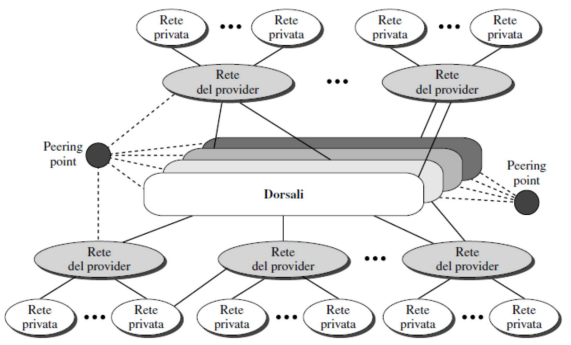
\includegraphics[scale=1]{internet.png}\\
\textbf{Peering point}: interconnessione tra due sistemi autonomi\\
\end{center}
\pagebreak
\subsection{Reti di accesso} Il collegamento tra l'utente ed il primo router di internet è detto \textbf{rete di accesso}.
\begin{list}{}{Può avvenire in 3 modi:}
\item \textbf{Tramite rete telefonica}: servizio dial-up, ADSL\ldots
\item \textbf{Tramite reti wireless}
\item \textbf{Collegamento diretto}, come collegamenti WAN dedicati ad alta velocità (aziende e università)
\end{list}
\section{Metriche di Riferimento}
Come misurare le prestazioni della rete?
\begin{list}{}{Tramite una serie di metriche:}
\item \textbf{Bandwith} o ampiezza di banda: è la larghezza dell'intervallo di frequenze utilizzato dal sistema trasmissivo (Hz).\\\textbf{Bitrate} o \textbf{transmission rate}: quantità di bit che possono essere trasmessi o ricevuti nell'unità di tempo (bit/secondo, bps)\\Il bitrate dipende dalla bandwidth e dalla tecnica trasmissiva utilizzata.
\item \textbf{Throughput}: la quantità di traffico che arriva realmente a destinazione nell'unità di tempo (al netto di perdite sulla rete, funzionamento dei protocolli ecc\ldots).\\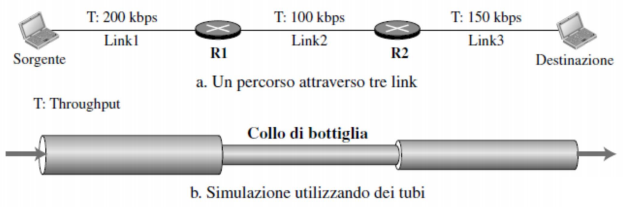
\includegraphics[scale=1]{throughput.png}\\Non è detto che corrisponda alla bandwidth perché ci potrebbe essere un collo di bottiglia.
\item \textbf{Latenza} o ritardo: il tempo richiesto affinché un messaggio arrivi a destinazione dal momento in cui il primo bit parte dalla sorgente.\\
\texttt{latenza = ritardo di propagazione + ritardo di trasmissione + ritardo di accodamento + ritardo di elaborazione}
\item \textbf{Perdita di pacchetti}. Come si può verificare?\\
\begin{multicols}{2}
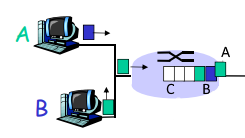
\includegraphics[scale=1]{ritpackets.png}\\

\columnbreak
A $\rightarrow$ pacchetti \textbf{in attesa} di essere trasmessi (\emph{ritardo})\\
B $\rightarrow$ pacchetti \textbf{accodati} (\emph{ritardo})\\
C $\rightarrow$ buffer \textbf{liberi} (se non ci sono buffer liberi, i pacchetti in arrivo vengono scartati, \emph{perdita})\\\\
I pacchetti da spedire vengono accodati nei buffer dei router. Di solito, il tasso di arrivo dei pacchetti sul router eccede le capacità del router di evaderli, quindi \textbf{i pacchetti si accodano in attesa del proprio turno}.
\end{multicols}
Il \textbf{ritardo di elaborazione} è dato dal controllo sui bit e dalla determinazione del canale di uscita (trascurabile)\\
Il \textbf{ritardo di accodamento} è dato dall'attesa di un pacchetto di essere trasmesso (B)\\
Il \textbf{ritardo di trasmissione} è il tempo impiegato per trasmettere un pacchetto sul link.\\\texttt{R$_{trasmissione}$ = R/L}\\
\texttt{R} = rate di trasmissione del collegamento, in bps\\
\texttt{L} = lunghezza del pacchetto in bit\\
Il \textbf{ritardo di propagazione} è il tempo impiegato da 1 bit per essere propagato da un nodo all'altro.\\\texttt{R$_{propagazione}$ = d/s}\\
\texttt{d} = lunghezza del collegamento\\
\texttt{s} = velocità di propagazione del collegamento (si usa la velocità della luce, circa 3 x 10$^{8}$ m/s)
\end{list}
\texttt{d$_{nodal}$ = d$_{proc}$ + d$_{queue}$ + d$_{trans}$ + d$_{prop}$}\\
\texttt{d$_{proc}$} = \textbf{ritardo di elaborazione}, pochi microsecondi\\
\texttt{d$_{queue}$} = \textbf{ritardo di accodamento}, dipende dalla congestione\\
\texttt{d$_{trans}$} = \textbf{ritardo di trasmissione}, \texttt{L/R} e significativo a lunga distanza\\
\texttt{d$_{prop}$} = \textbf{ritardo di propagazione}, \texttt{d/s}, da pochi microsecondi a centinaia di millisecondi\\
\section{Modelli Stratificati}
$https://elearning.di.unipi.it/pluginfile.php/27387/mod_resource/content/1/L02_introduzione_protocolli.pdf$
\paragraph{Perché usare un modello a strati} Per mandare dei dati da un host ad un altro comunicando su una rete, si devono eseguire una \textbf{serie di operazioni}: \textbf{trovare il percorso} di rete da attraversare, \textbf{decidere in che modo spedire e codificare} i dati, \textbf{risolvere eventuali problemi} di comunicazione e altro ancora.\\
Programmare ogni volta tutto il procedimento è un \textbf{lavoro estremamente complesso} e ripetitivo. Un modello a strati \textbf{astrae su più livelli il problema della trasmissione dati} in modo da fornire di volta in volta strumenti utili al programmatore per poter evitare di "\textit{reinventare la ruota}".
\paragraph{Definizioni generali} Nelle architetture di comunicazione a strati sono importanti una serie di definizioni:
\begin{list}{-}{}
\item Stratificazione
\item Information hiding
\item Separation of concern
\item Modello ISO/OSI
\item Stack TCP/IP
\end{list}
Tali definizioni verranno viste durante il corso.
\paragraph{Lo Strato} Uno \textbf{strato} è un \textbf{modulo interamente definito} attraverso i servizi, le interfacce e i protocolli che lo caratterizzano. Si indica anche col nome di livello.\\
Uno strato \texttt{n} \textbf{comunica direttamente} con lo strato \texttt{n} di un'altra unità tramite un \textbf{protocollo assegnato}. Lo stesso strato \texttt{n} può richiedere servizi allo strato \texttt{n-1} attraverso la \textbf{loro interfaccia}, e fornisce servizi allo strato \texttt{n+1} attraverso la \textbf{rispettiva interfaccia}.
\paragraph{Es. modello stratificato: sistema postale}\texttt{Vedi slide\\$https://elearning.di.unipi.it/pluginfile.php/27387/mod_resource/content/1/L02_introduzione_protocolli.pdf$, 48}\\
Dal livello più alto al livello più basso per la spedizione, viceversa per la ricezione. Un problema importante che si incontra quando si manda una lettera, ad esempio, dall'Italia al Giappone è la traduzione. In una \textbf{serie di passi}, in cui in ognuno viene \textbf{eseguito un particolare compito su un messaggio}, che viene poi \textbf{trasferito ad un altro livello}. Nell'esempio, la segretaria prepara lettera (traduce in giapponese e imbusta) affinché il postino la possa prendere. Però il "messaggio" della segretaria è "scritto" per essere interpretato dalla segretaria giapponese, il direttore italiano scrive per il direttore giapponese. \textbf{Messaggi di un livello del sistema che spedisce sono scritti per essere interpretati dal medesimo livello del sistema ricevente}.
\subsection{Perché stratificare} La stratificazione è molto utile per \textbf{scomporre il sistema complesso della gestione della comunicazione}. Prendo un sistema estremamente costoso da costruire per una singola coppia di aziende, quindi lo trasformo in strati così che il costo della singola lettera sia irrisorio.\\
\textbf{Definisco funzioni di base per effettuare trasferimento e agenti che le svolgono}.
\begin{list}{}{Principi di base:}
\item \textbf{Separation of Concern}\\\textbf{Far fare} ad un determinato strato \textbf{solo ciò che gli compete}, \textbf{delegando agli altri tutto ciò che è delegabile}
\item \textbf{Information Hiding}\\\textbf{Nascondo} ad un determinato strato \textbf{le informazioni non indispensabili allo svolgere della sua operazione}.
\end{list}

\paragraph{Esempio} Se traduco il modello postale nel modello a strati ho, ad esempio:\\
\begin{center}
\begin{multicols}{2}
Utente\\Segretaria\\Postino\\Smistamento\\Stazione\\
\columnbreak
Utente\\Segretaria\\Postino\\Smistamento\\Stazione\\
\end{multicols}
---Viaggio$\rightarrow$
\end{center}

\subsection{Smistamento Intermedio} Spedire un pacchetto che è destinato ad determinato livello intermedio. Quindi \textbf{arrivo fino al corrispondente livello intermedio per evitare che si possano esporre info sensibili}.
\subsection{Elementi fondamentali}
Gli \textbf{elementi fondamentali} del modello stratificato sono:
\begin{list}{}{}
\item Flusso dati
\item \textbf{Servizio}: una \textbf{funzione} che uno strato offre allo strato superiore, attraverso un'interfaccia.
\item Protocollo
\item \textbf{Interfaccia}: \textbf{insieme di regole} che governano il formato e il significato dei frame, pacchetti o messaggi che vengono \textbf{scambiati tra strati adiacenti della stessa entità}.
\end{list}
\textbf{I servizi indicano \textit{cosa} si può fare, le interfaccie regolano \textit{come} si può fare.}

\subsection{Modalità di Servizio}
\begin{list}{}{I \textbf{dati} possono essere scambiati in due modalità diverse:}
\item \textbf{Connection-Oriented}: il livello di trasferimento stabilisce una \textbf{connessione logica} tra due sistemi.
\begin{list}{--}{La connessione è quindi \textbf{gestita}:}
\item \textbf{Instaurazione} della connessione
\item \textbf{Trasferimento} dei dati
\item \textbf{Chiusura} della connessione
\end{list}
\item \textbf{Connectionless}: i dati vengono \textbf{trasferiti senza stabilire una connessione}.
\end{list}
\subsection{Vantaggi}
Il vantaggio più grosso è che \textbf{sviluppare il singolo strato è più semplice ed economico rispetto a sviluppare tutto il sistema complesso}. Questo perché \textbf{i servizi degli strati inferiori vengono usati da più entità che implementano gli strati superiori}.
\pagebreak
\section{Protocolli}
\paragraph{Cos'è un protocollo} Un \textbf{protocollo} è un \textbf{insieme di regole} che dice come comunicare ed esporre dati verso l'esterno. I protocolli \textbf{definiscono il formato e l'ordine dei messaggi inviati e ricevuti, con le azioni per trasmette e ricevere tali messaggi}.
\subsection{Incapsulamento} Processo in cui \textbf{aggiungo strati, "involucri" al messaggio originale che vengono man mano tolti alla destinazione}.
\section{OSI RM (Open Systems Interconnction Reference Model)}
Le prime reti erano chiuse, composte da tecnologie e protocolli proprietari. Alcuni esempi sono ARPANET, SNA (IBM), DNA (Digital). Non potevano intercomunicare tra loro, perché usavano \textbf{protocolli diversi}, erano costruite per servizi specifici (TELCO). Insorse quindi un obiettivo: creare un \textbf{modello di riferimento per sistemi aperti}, per permettere a qualsiasi terminale di poter comunicare mediante qualsiasi rete. C'era quindi necessità di \textbf{accordarsi sulle regole}.
\paragraph{OSI} L'OSI è una \textbf{collezione di protocolli aperti}: questo significa che i loro \textbf{dettagli sono pubblici} e i \textbf{cambiamenti vengono gestiti da un'organizzazione con partecipazione aperta al pubblico}. \textbf{Un sistema che implementa i protocolli aperti è un sistema aperto}.
\subsubsection{Pila di protocolli} L'\textbf{OSI} prevede \textbf{sette strati di protocolli}: 
\begin{list}{}{}
\item\textbf{7. Applicativo}: elaborazione dei dati
\item\textbf{6. Presentazione}: unificazione dei dati, preparazione del \textbf{pacchetto} da trasmettere/ricevere
\item\textbf{5. Sessione}:  controllo del dialogo tra gli host sorgente e destinazione.
\item\textbf{4. Trasporto}: offre il vero e proprio trasferimento dati tra gli host terminali, cioè \textbf{astrae la logica} con la quale si scambiano i dati tra host e gestisce gli errori. Realizza il \textbf{dialogo end-to-end}.
\item\textbf{3. Rete}: instradamento del traffico (principalmente router, offre il servizio di consegna attraverso il sistema distribuito dei nodi intermedi).
\item\textbf{2. Datalink}: consegna il frame tra le interfacce, interpretato dalla scheda di rete.
\item\textbf{1. Fisico}: modulazione del segnale elettrico per trasmettere correttamente il flusso di bit sul mezzo fisico.
\end{list}
I livelli \textbf{7-5} si possono raggruppare in più modi, principalmente sono gli strati di supporto all'elaborazione e all'interazione con l'utente. Sono livelli \textbf{software}\\
I livelli \textbf{4-1} sono \textbf{software e hardware}. Sono strati di supporto alla rete e all'infrastruttura trasmissiva, cioè gestiscono la vera e propria trasmissione dei dati.
\pagebreak
\section{Flusso dell'Informazione}
Per le reti, l'informazione ha origine al \textbf{livello applicativo}, che la genera per mandarla in remoto. Una volta generata, essa discende i vari livelli fino al canale fisico e ogni livello \textbf{aggiunge} all'informazione ricevuta dal livello superiore \textbf{una -- o più -- propria sezione informativa} sotto forma di \textbf{header}, contenente informazioni esclusive di quel livello. Per l'informazione ricevuta, si segue il \textbf{cammino inverso}, quindi dal basso verso il livello applicativo, e ogni livello "spacchetta" l'header del livello corrispondente, ne legge le informazioni esclusive e lo gestisce appositamente.\\Il \textbf{processo di incapsulamento} è quindi \textbf{reversibile}: ogni livello esegue una operazione di incapsulamento su dati già incapsulati dal livello precedente, in modo tale da garantire la possibilità di estrarre i dati precedentemente incapsulati.\\
\
\begin{center}
\rule{6.8cm}{1pt}\\
HEADER ||| DATA ||| TRAILER\\
\rule{6.8cm}{1pt}\\
\end{center}
\textbf{Header}: qualificazione del pacchetto per questo livello\\
\textbf{Data}: payload proveniente dal livello superiore\\
\textbf{Trailer}: generalmente usato in funzione del trattamento dell'errore\\
\begin{center}
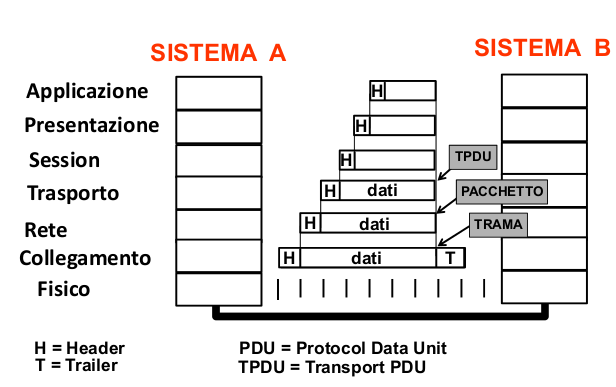
\includegraphics[scale=0.75]{incapsulamento.png}
\end{center}
\pagebreak
\section{Stack protocollare TCP/IP}
Il \textbf{TCP/IP} è una famiglia di protocolli attualmente utilizzati in internet. Si tratta di una \textbf{gerarchia di protocolli} costituita da \textbf{moduli interagenti}, ciascuno con funzioni specifiche.
\paragraph{Gerarchia} Con il termine \textbf{gerarchia} s'intende che ciascun protocollo di livello superiore è \textbf{supportato dai servizi forniti dai protocolli di livello inferiore}. Cioè un protocollo a livello \texttt{n} realizza le sue funzionalità grazie ai protocolli a livello \texttt{n-1}.
\begin{multicols}{2}
\subsection{I Livelli}
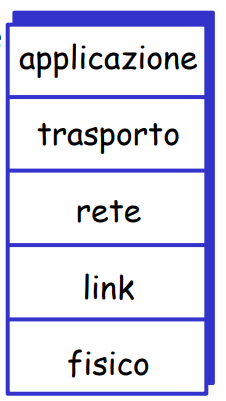
\includegraphics[scale=0.8]{stacktcpip.png}
\columnbreak


Lo stack TCP/IP in origine era intesa come \textbf{quattro livelli software} sovrastanti \textbf{un livello hardware}. Oggi è intesa come semplicemente \textbf{composta da 5 livelli}
\paragraph{Livello Applicativo} Il livello più alto, con il quale interagisce l'utente\\
Identificativi risorse: URL, URI, URN\\
Il web: user agents, http: request, response, connessioni persistenti, GET, POST, PUT, DELETE, status code, proxy server, caching\\
FTP: connessioni dati e di controllo, rappresentazione\\
TELNET\\
Posta elettronica: SMTP, POP3, IMAP\\
DNS e risoluzioni nomi: gerarchia nomi, risoluzione iterativa e ricorsiva, formato pessaggi, nslookup...
\paragraph{Livello Trasporto} Livello al quale si definisce la codifica e il protocollo di trasporto\\
Servizi: mux demux, controllo errore, connectionless\\
TCP: formato segmenti, gestione connessione, controllo flusso e congestione\\
UDP: formato segmenti
\paragraph{Livello Rete} Dove si gestisce l'indirizzamento dei vari host\\
Strato di rete e funzioni\\
Indirizzamentoi IP: classful IPv4, NAT, sottoreti e maschere, classless, CIDR\\
Risoluzione IP e MAC, ARP\\
IPv4: formato datagramma ip, frammentazione\\
Routing IP e istradamento\\
Introduzione IPv6
\paragraph{Livello Link} Trasferimento dati tra elementi di rete vicini\\
Ethernet
\paragraph{Livello Fisico} Bit sul filo
\end{multicols}
\pagebreak
\section{Livello Applicativo}
\paragraph{Applicazioni e processi} Le applicazioni possono essere composte da \textbf{vari processi distribuiti} comunicanti fra loro. Un \textbf{processo} sono programmi eseguiti degli host di una rete. Due processi possono anche comunicare all'interno dello stesso host attraverso la \textbf{comunicazione inter-processo} (definita dal S.O.).\\
Nella \textbf{comunicazione a livello applicativo fra due host di una rete}, due o più processi vengono eseguiti da ciascuno degli host comunicanti e \textbf{si scambiano messaggi}.\\\\
I livelli applicazione dei due host \textbf{si comportano come se esistesse un collegamento diretto} attraverso cui mandare e ricevere messaggi.
\subsection{Protocollo a Livello Applicativo}
Un protocollo di livello applicativo \textbf{definisce}:
\begin{list}{}{}
\item \textbf{Tipi di messaggi} scambiati a quel livello, ad esempio di richiesta o di risposta
\item \textbf{Sintassi} dei vari tipi di messaggi, cioè i campi
\item \textbf{Semantica} dei campi
\item \textbf{Regole} per determinare quando e come un processo invia o risponde ai messaggi
\end{list}
\subsection{Paradigmi}
I due programmi applicativi devono essere entrambi in grado di richiedere e offrie servizi oppure ognuno deve occuparsi di uno dei due compiti?
\paragraph{Client-Server} Un \textbf{numero limitato} di \textbf{processi server} che \textbf{offrono} un servizio, in esecuzione \textbf{in attesa di richieste} dai \textbf{processi client}, che \textbf{richiedono} servizi.
\subparagraph{Client} \textit{Parla per primo}, cioè inizia il contatto con il server. Tipicamente richiede un servizio al server, ad esempio: per il web il client è implementato nel browser, per l'e-mail è implementato nel mail reader.
\subparagraph{Server} Fornisce al client il servizio richiesto e \textbf{rimane sempre attivo}. Ad esempio: un web server invia le pagine richieste, un mail server smista ed invia le mail.
\paragraph{Peer-to-Peer} Host \textbf{peer} che possono \textbf{offrire servizi e inviare richieste}.
\paragraph{Misto} Un misto tra i due paradigmi sopra.
\subsection{Componenti di un'Applicazione di Rete}
Due esempi
\paragraph{Web}
\begin{list}{-}{Composto da:}
\item Web Browser, sul \textbf{client}
\item Web \textbf{Server}
\item \textbf{Standard per il formato} delle risorse (pagine ecc.)
\item \textbf{Protocollo} HTTP
\end{list}
\paragraph{Posta Elettronica}
\begin{list}{-}{Composta da:}
\item Programmi di lettura e scrittura sul \textbf{client}
\item \textbf{Server} di posta in internet
\item \textbf{Standard per il formato} dei messaggi
\item \textbf{Protocolli} SMTP, POP3 ecc.
\end{list}
\subsection{Terminologia}
\paragraph{API} \textbf{Application Programming Interface}: si tratta di un \textbf{insieme di regole} che un programmatore deve rispettare per utilizzare delle risorse.
\paragraph{Socket} Una \textbf{API} che funge da \textbf{interfaccia} tra gli strati di applicazione e di trasporto. A tutti gli effetti è la \textbf{API di internet per eccellenza}, due processi comunicano mandando dati sul socket e leggendoli da esso. Forma una \textbf{connessione logica}, l'invio e ricezione dei dati sono responsabilità del S.O. e del TCP/IP.
\subsection{Identificazione di un Processo}
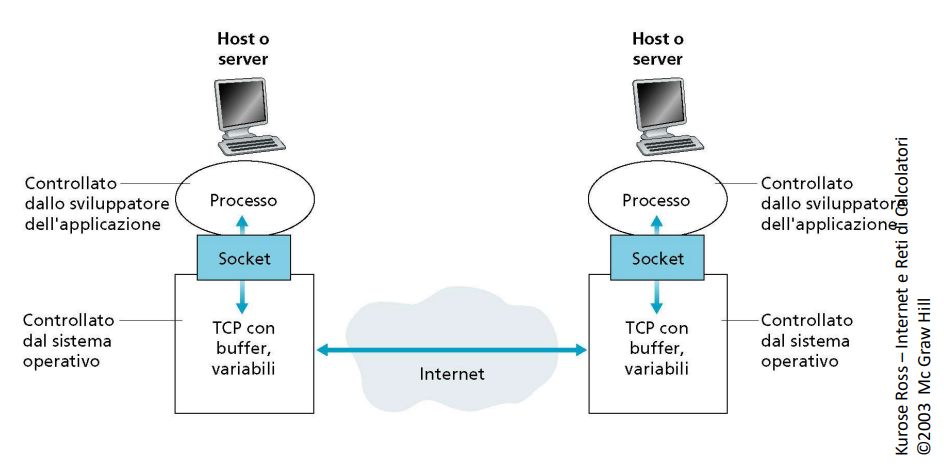
\includegraphics[scale=0.73]{identifprocesso.png}
I servizi di trasporto sono offerti al livello applicativo tramite le API. Ogni servizio di transport è \textbf{usato simultaneamente} da più processi application.\\
Come identifico i processi di livello application \textbf{di host diversi}? Serve un identificativo che identifichi sia l'host che il processo.\\
$\rightarrow$ Coppie \texttt{<Indirizzo IP, Numero di porta>}
\begin{center}
\fbox{
        \fbox{\parbox{6cm}{Indirizzo IP [32bit]}}
		\fbox{\parbox{4cm}{Numero di porta [16 bit]}}
}
\end{center}
\subsection{Esempio di API: TCP}
\begin{lstlisting}
Connection TCPopen(IPAddress, int)	//per aprire una connessione
void TCPsend(Connection, Data)		//per spedire dati su una connessione
Data TCPreceive(Connection)		//per ricevere dati da una connessione
void TCPclose(Connection)		//per chiudere una connessione
int TCPbind(int)			//per richiedere l'assegnazione della porta su
					//cui attendere le richieste di connessione

void TCPunbind(int)			//per liberare la porta assegnata
Connection TCPaccept(int)		//per attendere le richieste di connessione

//Connection: identificata da una quadrupla
//Astraggo dalle possibili eccezioni sollevate e dal loro trattamento
\end{lstlisting}
\pagebreak
\subsection{Uso dei Servizi di Trasporto}
Una coppia di processi fornisce servizi agli utenti di Internet, siano questi persone o applicazioni. La coppia di processi, tuttavia, \textbf{deve utilizzare i servizi offerti dal livello di trasporto} per la comunicazione, poiché non vi è una comunicazione fisica a livello applicativo. Le applicazioni di retesono quindi \textbf{realizzate \textit{sopra} ai servizi di trasporto dati}.\\
Nel livello trasporto dello stack protocollare TCP/IP sono previsti \textbf{due protocolli di trasporto principali}:
\begin{list}{}{}
\item \textbf{TCP} Transfer Control Protocol
\begin{list}{}{}
\item \textbf{Connection-Oriented}: è richiesto un setup tra client e server
\item Trasporto \textbf{affidabile} tra mittente e destinatario
\item \textbf{Controllo del flusso}: il mittente non \textit{inonderà} di dati il destinatario
\item \textbf{Controllo di congestione}: \textit{limita} il mittente quando la rete è satura
\item Non offre garanzie di timing né di ampiezza minima di banda
\end{list}
\item \textbf{UDP} User Datagram Protocol
\begin{list}{}{}
\item \textbf{Connectionless}
\item Trasporto \textbf{non affidabile}
\item \textbf{NO} controllo del flusso
\item \textbf{NO} controllo di congestione
\item \textbf{NO} garanzie di timing o di ampiezza minima di banda
\item \textit{Quindi quali applicazioni usano UDP, e perché?}
\end{list}
\end{list}
\paragraph{Che tipo di trasporto richiede un'applicazione?}
\subparagraph{Throughput} Anche detta \textbf{banda}, è la frequenza alla quale il processo mittente può inviare i bit al processo ricevente. Alcune applicazioni (es. multimedia) richiedono una \textbf{banda minima} per essere efficaci, altri (\textbf{elastic apps}) usano la banda che trovano a disposizione.\\Velocità di trasferimento $\neq$ velocità di propagazione
\subparagraph{Perdita di dati} Alcune applicazioni (es. audio) possono tollerare alcune perdite, altre (es. telnet, trasferimento file) richiedono un trasferimenti dati \textbf{affidabile} al 100%
\subparagraph{Timing} Alcune applicazioni (es. teleconferenze, videogame) richiedono un basso ritardo per essere efficaci
\begin{center}
\begin{tabbing}
\begin{tabular}{c | c c c }
\textbf{Applicazione} & \textbf{Tolleranza alla perdita dati} & \textbf{Throughput} & \textbf{Sensibilità al tempo}\\\hline\\
Trasferimento file & No & Variabile & No\\\\
Posta Elettronica & No & Variabile & No\\\\
Documenti Web & No & Variabile & No\\\\
Audio/Video in tempo reale & Si & \begin{tabular}{@{}c@{}}Audio: 5Kbps -- 1 Mbps\\Video: 10Kbps -- 5MKbps\end{tabular} & Si, centinaia di millisecondi\\\\
Audio/Video memorizzati & Si & \begin{tabular}{@{}c@{}}Audio: 5Kbps -- 1 Mbps\\Video: 10Kbps -- 5MKbps\end{tabular} & Si, pochi secondi\\\\
Videogame & Si & Fino a pochi Kbps & Si, centinaia di millisecondi\\\\
Messaggistica istantanea & No & Variabile & Si e no
\end{tabular}
\end{tabbing}
\end{center}
\pagebreak

\begin{center}
\begin{tabbing}
\begin{tabular}{c | c c }
\textbf{Applicazione} & \textbf{Protocollo a Livello Applicativo} & \textbf{Protocollo di Trasporto}\\\hline\\
Posta Elettronica & SMTP (RFC 2821) & TCP\\
Accesso a terminali remoti & Telnet (RFC 854) & TCP\\
Web & HTTP (RFC 2616) & TCP\\
Trasferimento file & FTP (RFC 959) & TCP\\
Streaming multimediale & HTTP (es. YouTube), RTP (RFC 1889) & TCP o UDP\\
Telefonia internet & SIP, RTP, proprietario (es. Skype) & Tipicamente UDP
\end{tabular}
\end{tabbing}
\end{center}
\section{Applicazioni Web e HTTP}
\subsection{Terminologia}
\paragraph{WEB} Consiste di \textit{oggetti} indirizzati da un \textbf{URL} (Uniform Resource Locator)
\paragraph{Pagine Web} Solitamente formate da: \textit{pagine WEB} (HTML, Javascript\ldots) e diversi \textbf{oggetti referenziati} (altre pagine, immagini, script\ldots)
\paragraph{Browser} Lo user agent per il web, ad esempio: Chrome, Firefox, Netscape, Lynx
\paragraph{Web server} Il server per il web, ad esempio: Apache, MS Internet Information Server
\subsection{Uniform Resource Identifier}
Una \textbf{URI} è una \textbf{forma generale per identificare una risorsa presente sulla rete} (IETF RFC 2396: \textit{una Uniform Resource Identifier è una stringa compatta di caratteri usata per identificare una risorsa astratta o fisica}).\\
La sintassi di uno URI è stata progettata ponendo la \textbf{trascrivibilità globale} come uno degli obiettivi principali: utilizza caratteri da un \textbf{alfabeto molto limitato} (es. le lettere dell'alfabeto latino base, numeri e qualche carattere speciale).\\
Uno URI può essere \textbf{rappresentato in molti modi}, ad esempio: inchiostro su carta, pixel su schermo, sequenza di ottetti\ldots L'\textbf{interpretazione di uno URI dipende soltanto dai caratteri utilizzati e non da come essi vengono rappresentati} nel protocollo di rete.
\subparagraph{Uniform} \textbf{Uniformità della sintassi} dell'identificatore, anche se i meccanismi per accedere alle risorse possono variare.
\subparagraph{Resource} Qualsiasi cosa abbia un'identità: documento, servizio, immagine, collezione di risorse\ldots
\subparagraph{Identifier} Oggetto che può agire da riferimento verso qualcosa che ha identità
\paragraph{}Esistono due tipi di URI:
\begin{list}{}{}
\item \textbf{URL} Uniform Resource Locator: sottotipo di URI che identifica una risorsa attraverso il suo \textbf{meccanismo di accesso primario}, ad esempio la \textit{posizione} nella rete.\\
\begin{list}{URL}{Esempi:}
\item \texttt{https://doi.org/10.1109/LCN.1988.10239}
\item \texttt{ftp://ftp.is.co.za/rfc/rfc1808.txt}
\item \texttt{https://www.apple.com/index.html}
\end{list}
\item \textbf{URN} Uniform Resource Name: sottotipo di URI che devono essere \textbf{globalmente univoci e persistenti}, anche quando la risorse cessa di esistere o di essere disponibile.\\
\begin{list}{URN}{Esempi:}
\item \texttt{urn:oasis:names:specification:docbook:dtd:xml:4.1.2:}
\item \texttt{urn:doi:10.1109/LCN.1988.10239}
\end{list}
\end{list}
\pagebreak
\subsubsection{Sintassi}
La sintassi di un URI è \textbf{organizzata gerarchicamente}, con le componenti \textbf{elencate in ordine decrescente} di importanza da sinistra a destra.\\
Una \textbf{URI assoluta} può essere formata da \textbf{quattro} componenti\\
\begin{center}
\texttt{<scheme>://<authority><path>?<query>}
\end{center}
\begin{list}{}{}
\item \texttt{<scheme>} \textbf{Obbligatorio}, schema per identificare la risorsa.\\
Lo URI scheme \textbf{definisce il namespace} dello URI, quindi potrebbe porre ulteriori vincoli su sintassi e semantica degli identificatori che usano quello schema. Nonostante molti URL scheme prendono il nome da protocolli, \textbf{questo non implica che l'unico modo di accedere} la risorsa dello URL \textbf{sia attraverso il protocollo specificato}.
\item \texttt{<authority>} Elemento gerarchico per richiamare un'authority così che la gestione del namespace definito sia delegato a quella authority. Il \textbf{nome di dominio} di un host o il suo \textbf{indirizzo IP} in notazione puntata decimale.\\
\texttt{authority = [userinfo@]host[:port]}
\item \texttt{<path>} Contiene dati specifici per l’authority (o lo scheme) e \textbf{identifica la risorsa nel contesto} di quello schema e di quella autorità. Può consistere in una sequenza di segmenti.
\item \texttt{<query>} L'interrogazione o i dati da passare alla risorsa richiesta
\end{list}
\begin{list}{}{Esempi:}
\item \texttt{foo://example.com:8042/over/there?name=ferret\#nose}
\begin{list}{}{}
\item \texttt{scheme = foo}
\item \texttt{authority = example.com:8042}
\item \texttt{path = /over/there}
\item \texttt{query = name=ferret}
\item \texttt{fragment = nose}
\end{list}
\item \texttt{urn:example:animal:ferret:nose}
\begin{list}{}{}
\item \texttt{scheme = urn}
\item \texttt{path = example:animal:ferret:nose}
\end{list}
\item \texttt{http://maps.google.it/maps/place?q=largo+bruno+pontecorvo+pisa\&hl=it}
\begin{list}{}{}
\item \texttt{scheme = http}
\item \texttt{authority = maps.google.it}
\item \texttt{path = /maps/place}
\item \texttt{query = q=largo+bruno+pontecorvo+pisa\&hl=it}
\end{list}
\end{list}
\subsubsection{Assolute e Relative}
Le URI possono essere assolute o relative.
\subparagraph{URI Assoluta} Identifica una risorsa \textbf{indipendentemente dal contesto} in cui è usata.
\subparagraph{URI Relativa} Informazioni per \textbf{identificare una risorsa in relazione ad un'altra URL} (è priva di \texttt{scheme} e \texttt{authority}). \textbf{Non viaggiano sulla rete}, sono interpretate dal browser in relazione al documento di partenza.
\pagebreak
\paragraph{Esempio di URI relativa}
Sia \texttt{http://a/b/c/d;p?q} il documento di partenza, allora
\begin{list}{}{}
\item \texttt{g} = \texttt{http://a/b/c/g}
\item \texttt{/g} = \texttt{http://a/g}
\item \texttt{//g} = \texttt{http://g}
\item \texttt{?y} = \texttt{http://a/b/c/?y}
\item \texttt{\#s} = \textit{documento corrente}\texttt{\#s}
\item \texttt{g;x?y\#s} = \texttt{http://a/b/c/g;x?y\#s}
\item \texttt{..} = \texttt{http://a/b/}
\item \texttt{../../g} = \texttt{http://a/g}
\end{list}
\section{HTTP}
Lo HTTP è usato dal 1990 come \textbf{protocollo di trasferimento per il World Wide Web}. Definito nel seguente modo (RFC 2068, RFC 2616): \textit{\textbf{procollo di livello applicazione} per sistemi di informazione distribuiti, collaborativi ed impermediali}.\\
Protocollo \textbf{generico}, \textbf{stateless} e \textbf{object-oriented} che può essere usato per molte attività, come name server e sistemi distribuiti di gestione oggetti, attraverso l'estensione dei suoi \textbf{request methods} (comandi). Una funzionalità dell'HTTP è la rappresentazione del tipo di dati, consentendo al sistema di essere \textbf{costruito indipendentemente dai dati che vengono trasferiti}.
\subsection{HTTP URL}
Lo schema \texttt{http} è usato per accedere alla risorsa attraverso il protocollo HTTP.
\paragraph{Sintassi} La sintassi per un URL http è:\\
\begin{center}
\texttt{http\_URL = http://host[:port][path]}
\end{center}
\begin{list}{}{}
\item \textbf{Host}: un dominio, hostname o indirizzo IP in forma decimale puntata di Internet.
\item \textbf{Porta}: un numero, se omessa viene usata la porta 80.
\end{list}
La risorsa è localizzata nel server in ascolto per connessioni TCP su quella porta di quell'host. Il path specifica la \textbf{Request-URI}.
\subsection{Caratteristiche}
Il protocollo HTTP è un protocollo \textbf{request/response}: la \textbf{connessione} viene \textbf{iniziata dal client}, che invia un \textbf{messaggio di request} al quale il server risponde con una \textbf{response}.\\
In quanto \textbf{generico e stateless} le coppie \textbf{richiesta/risposta sono indipendenti}.
\subsubsection{Modello} Il modello del protocollo HTTP è \textbf{client-server}:
\begin{list}{}{}
\item \textbf{Client}: browser che richiede, riceve e visualizza oggetti web.\\Stabilisce una connessione con il server e invia una \textbf{richiesta sotto forma di request-method, URI e versione di protocollo}, seguito da un messaggio.
\item \textbf{Server}: web server che invia oggetti in risposta ad una richiesta.\\Accetta le connessioni e serve le richieste rispondendo con i dati richiesti.
\end{list}
\subsubsection{Connessioni} Una \textbf{connessione} è un \textbf{circuito logico di livello trasporto} stabilito tra due programmi applicativi per comunicare tra loro.
\paragraph{Non-Persistent Connection} \texttt{http1.0: RFC 1945}\\Viene stabilita una \textbf{connessione TCP separata} per raggiungere ogni URL. \textbf{Aumenta il carico} sui server HTTP e \textbf{può causare congestioni su Internet} (questo perché, ad esempio, se vengono usate tante immagini allora si creano richieste multiple del solito server in un breve lasso di tempo).
\paragraph{Persistent Connection} \texttt{http1.1: RFC 2616}\\Se non è indicato altrimenti, il client può \textbf{assumere che il server manterrà una connessione persistente}.\\Lo standard specifica un \textbf{meccanismo con il quale} un client o un server \textbf{può segnalare la chiusura di una connessione TCP} (il campo \texttt{connection} nell'header). Una volta che la chiusura viene segnalata, il cliente \textbf{non deve più mandare richieste} su quella connessione.
\subsection{Esempio HTTP}
\texttt{Vedi slide}\footnote{https://elearning.di.unipi.it/pluginfile.php/27477/mod\_resource/content/2/L03\_Applicativo\_HTTP.pdf, slide 34}
\subsection{Messaggi HTTP}
\begin{center}
\texttt{generic-message = start-line *message-header CRLF [message-body]\\
start-line = Request-Line | Status-Line}
\end{center}
La \texttt{start-line} distingue \textbf{request} da \textbf{response}.\\\\
\textbf{HTTP Request Message}\\
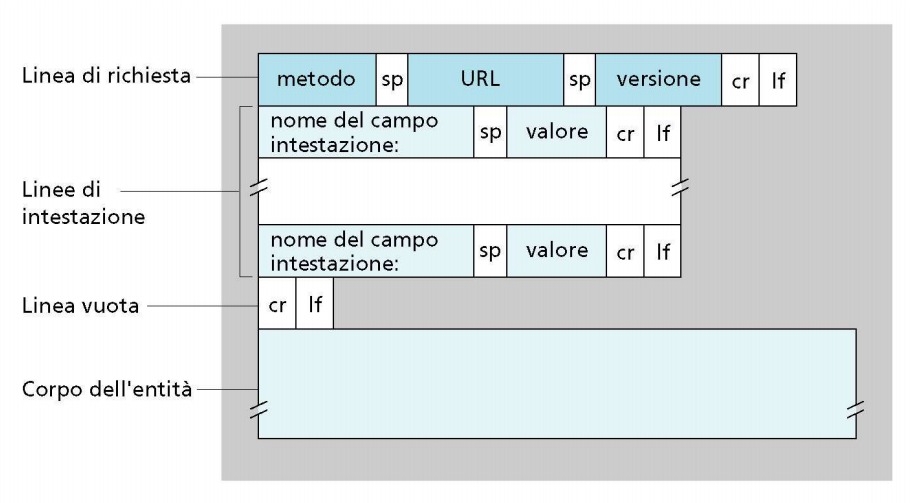
\includegraphics[scale=0.75]{httpmessage.png}\\
\textbf{HTTP Response Message}\\
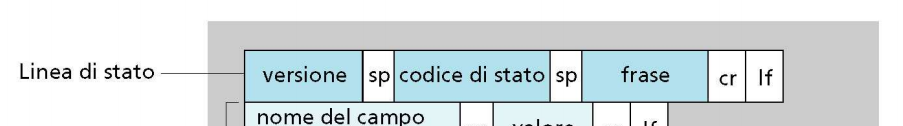
\includegraphics[scale=0.75]{httpresponse.png}
\pagebreak
\paragraph{HTTP Request} \texttt{Request-Line *( general-header | request-header | entity-header ) CRLF [message-body]}
Ad esempio:\\
\texttt{GET /pub/WWW/TheProject.html HTTP/1.1\\
Host: www.w3.org\\
Connection: close\\
User Agent: Mozilla/4.0\\
Accept-language: it\\\\
(Body)}
\subparagraph{HTTP Request Line} \texttt{Request-Line = Method SP Request-URI SP HTTP-Version CRLF}\\\texttt{GET http://www.w3.org/pub/WW/TheProject.html HTTP/1.1}
\begin{list}{}{}
\item \texttt{Method = GET}
\item \texttt{Request-URI = http://www.w3.org/pub/WW/TheProject.html}
\item \texttt{HTTP-Version = HTTP/1.1}
\end{list}
\texttt{Method = "OPTIONS" | "GET" | "HEAD" | "POST" | "PUT" | "DELETE" | "TRACE" | extension-method}\\
\begin{list}{}{}
\item \textbf{Method}: indica il \textbf{metodo che deve essere eseguito} sulla risorsa identificata dal \texttt{Request-URI}. \textbf{Case sensitive}.
\item \textbf{HTTP-Version}: indicare la versione del protocollo è pensato per consentire al mittente di indicare il formato di un messaggio e la sua capacità di capire il resto della comunicazione HTTP.
\item Le \textbf{URI} sono stringhe formattate in modo semplice che identificano una risorsa di rete.
\subsection{Header}
Gli \textbf{header} sono insiemi di coppie $<$nome:valore$>$ che \textbf{specificano alcuni parametri} del messaggio trasmesso o ricevuto.
\begin{list}{}{}
\item \textbf{General header} Relativi alla trasmissione
\begin{list}{}{}
\item \textbf{Data}: data e ora di generazione del messaggio
\item \textbf{Connection}: consente al mittente di specificare le opzioni desiderate per quella particolare connessione. L'opzione "close" segnala che la connessione verrà chiusa al completamento della response
\item \textbf{Transfer-encoding}: indica quale (se presente) tipo di trasformazione è stata applicata al message body per trasferirlo correttamente dal mittente al destinatario (chunked, gzip\ldots)
\item \textbf{Cache Control}
\begin{list}{}{}
\item \textbf{Public} Indica che la response è cachable in qualsiasi cache
\item \textbf{Private} Indica che tutte o parti della response sono destinate ad un singolo utente e \textbf{non devono essere} memorizzate in una cache condivisa (shared cache). Una cache privata (non-shared) potrebbe memorizzare la response
\item \textbf{no-cache} Indica che tutte o parti della response \textbf{non devono essere memorizzate in nessuna cache}
\end{list}
\end{list}
\texttt{general-header = Cache-Control | Connection | Date | Pragma | Transfer-Encoding | Upgrade | Via}\\Questi header si applicano \textbf{a tutto il messaggio}. Esempi:
\begin{list}{}{}
\item \texttt{Date: Tue, 15 Nov 1994 08:12:31 GMT}
\item \texttt{Connection: close}
\item \texttt{Transfer-Encoding: chunked}
\end{list}
\item \textbf{Entity header} Relativi all'entità trasmessa\\Content-type, Content-length, data di scadenza\ldots
\item \subsubsection{Request header} Relativi alla richiesta\\Chi fa la richiesta, a chi viene fatta, che tipo di caratteristiche è in grado di accettare il client, autorizzazione\ldots consente al client di passare \textbf{informazioni aggiuntive} a proposito della richiesta o del client stesso al server. Questi campi agiscono come \textbf{modificatori di richiesta}, con \textbf{semantica equivalente a quella dei parametri} di un metodo.\\
\texttt{request-header = Accept | Accept-Charset | Accept-Encoding | Accept-Language | Authorization | Proxy-Authorization | From | Host | If-Modified-Since | If-Unmodified-Since | If-Match | If-None-Match | If-Range | Max-Forwards | Range | Referer | User-Agent}\\
\begin{list}{}{}
\item \textbf{Accept} Specifica che tipi di media sono accettabili nella response. Parametro \texttt{q} per indicare un fattore di qualità relativo, default a 1.
\item \textbf{Accept-Charset} Indica il set di caratteri accettato per la risposta
\item \textbf{Accept-Encoding} Tipi di trasformazioni accettate (es. compressione)
\item
\item \texttt{Accept: text/plain;q=0.5, text/html, text/x-dvi;q=0.8, text/x-c}
\item \texttt{Accept-Charset: iso-8859-5, unicode-1-1;q=0.8}
\item \texttt{Accept-Encoding: compress, gzip}
\end{list}
\begin{list}{}{(Alcuni) metodi request:}
\item \textbf{OPTIONS} Richiede \textbf{solo le opzioni di comunicazione} associate ad un URL o al server stesso (capacità, metodi esposti ecc.). Un esempio:\\
\texttt{OPTIONS http://192.168.11.66/manual/index.html HTTP/1.1\\host: 192.168.11.66\\
Connection: close\\\\
HTTP/1.1 200 OK\\
Date: Sun, 14 May 2000 19:52:12 GMT\\
Server: Apache/1.3.9 (Unix) (Red Hat/Linux)\\
Content-Length: 0\\
Allow: GET, HEAD, OPTIONS, TRACE\\
Connection: close\\}
\item \textbf{GET} Richiede il trasferimento di una risorsa identificata da un URL o le operazioni associate all'URL stessa. Un esempio:\\
\texttt{GET http://192.168.11.66 HTTP/1.1\\
host: 192.168.11.66\\
Connection: close}\\\\
Response\\
\texttt{HTTP/1.1 200 OK\\
Date: Sun, 14 May 2000 19:57:13 GMT\\
Server: Apache/1.3.9 (Unix) (Red Hat/Linux)\\
Last-Modified: Tue, 21 Sep 1999 14:46:36 GMT\\
ETag: "f2fc-799-37e79a4c"\\
Accept-Ranges: bytes\\
Content-Length: 1945\\
Connection: close\\
Content-Type: text/html\\\\
<!DOCTYPE HTML PUBLIC "-//W3C//DTD HTML 3.2\\
Final//EN">\\
<HTML>\ldots\\}
Sono possibili \textbf{GET condizionali e parziali}. Esempio di GET condizionale:\\
\texttt{GET http://192.168.11.66 HTTP/1.1\\
Host: 192.168.11.66\\
If-Modified-Since: Tue, 21 Sep 1999\\
14:46:36 GMT}\\\\
Response:\\
\texttt{HTTP/1.1 304 Not Modified\\
Date: Wed, 22 Sep 1999 15:06:36 GMT\\
Server: Apache/1.3.9 (Unix) (RedHat/Linux)}\\
\item \textbf{HEAD} Simile al GET, ma il server \textbf{non trasferisce il body} nella response. Utile per controllare lo stato dei documenti (validità, modifiche\ldots). Un esempio:\\
\texttt{HEAD http://192.168.11.66 HTTP/1.1\\
host: 192.168.11.66\\
Connection: close}\\\\
Response (notare la somiglianza con GET, esclusa la mancanza qua del body):\\
\texttt{HTTP/1.1 200 OK\\
Date: Sun, 14 May 2000 20:02:41 GMT\\
Server: Apache/1.3.9 (Unix) (Red Hat/Linux)\\
Last-Modified: Tue, 21 Sep 1999 14:46:36 GMT\\
ETag: "f2fc-799-37e79a4c"\\
Accept-Ranges: bytes\\
Content-Length: 1945\\
Connection: close\\
Content-Type: text/html}\\
\item \textbf{POST} Serve per \textbf{inviare dal client al server} informazioni inserite nel body del messaggio.\\In teoria lo standard dice che il metodo POST è usato per richiedere che il server \textbf{accetti l'entità racchiusa nella richiesta come nuovo suboordinato della risorsa identificata} dallo Request-URI nel Request-Line.\\\textbf{Nella pratica}, \textbf{la funzionalità effettiva del metodo POST} è \textbf{determinata dal server} e solitamente dipende dalla Request-URI.\\
\item \textbf{DELETE} Il client \textbf{chiede di cancellare una risorsa identificata} dalla Request-URI.\\Solitamente non attivo su server pubblici.\\
\item \textbf{PUT} Il client \textbf{chiede di creare/modificare una risorsa identificata} dalla Request-URI. Dopo posso usare una GET per recuperarla.\\Solitamente non attivo su server pubblici.
\end{list}
\item \textbf{Response header} Nel messaggio di risposta\\Server, autorizzazione richiesta\ldots
\end{list}
\paragraph{Safe Methods} Metodi che \textbf{non hanno effetti collaterali} (es. non modificano la risorsa): GET, HEAD, OPTIONS, TRACE
\paragraph{Idempotent Methods} Metodi che \textbf{non hanno effetti ulteriori se vengono fatti N $>$ 0 richieste identiche}: GET, HEAD, PUT, DELETE, OPTIONS, TRACE
\end{list}
\pagebreak
\subsection{HTTP Response}
\begin{center}
\texttt{Response = Status-Line *( general-header | response-header | entity-header ) CRLF [message-body]}
\end{center}
Un esempio:\\
\texttt{HTTP/1.1 200 OK\\
Date: Sun, 14 May 2000 23:49:39 GMT\\
Server: Apache/1.3.9 (Unix) (Red Hat/Linux)\\
Last-Modified: Tue, 21 Sep 1999 14:46:36 GMT}\\
\paragraph{Status-Line} La prima linea del messaggio di risposta.\\
\texttt{Status-Line = HTTP-Version SP Status-Code SP Reason-Phrase CRLF}\\Esempio: \texttt{HTTP/1.1 200 OK}
\subparagraph{Status-Code} Intero a 3 cifre, risultato del tentativo di comprendere e soddisfare la richiesta.\\\begin{center}
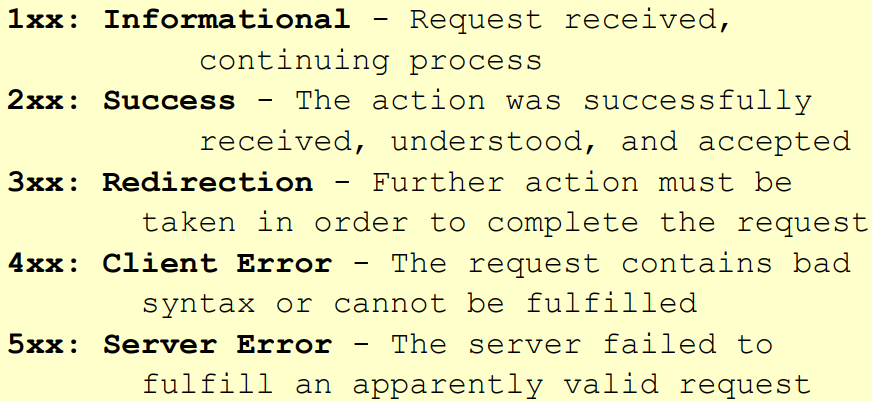
\includegraphics[scale=0.5]{httpresponsecode.png}\\\texttt{http://www.w3.org/Protocols/rfc2616/rfc2616-sec10.html}
\end{center}
\subparagraph{Reason-Phrase} Ha l'obiettivo di fornire una breve descrizione testuale dello Status-Code. Lo Status-Code è indirizzato ai computer mentre la Reason-Phrase è per gli umani.
\subsubsection{Response Headers} Il campo response-header consente al server di passare ulteriori informazioni sulla response. Questi campi dell'header forniscono informazioni sul server e sull'accesso alla risorsa identificata dallo Request-URI.\\
\texttt{response-header = Age | Location | Proxy-Authenticate | Public | Retry-After | Server | Vary | Warning | WWW-Authenticate}\\\\Esempio:\\
\texttt{Age: 150 // età del doc. se tramite Proxy\\
Location: http://www.w3.org/pub/WWW/People.html\\
Server: CERN/3.0 libwww/2.17}
\begin{list}{}{}
\item \textbf{Age} Una stima in secondi del tempo passato dalla generazione della risposta dal server di origine
\item \textbf{Location} Usato per reindirizzare il ricevente verso una destinazione diversa dalla Request-URI per il completamento della richiesta o l'identificazione di una nuova risorsa
\item \textbf{Server} Informazioni sul software usato dal server d'origine per gestire la richiesta
\end{list}
\subsection{Negoziazione del contenuto}
Le risorse possono essere \textbf{disponibili in multiple rappresentazioni}, ad esempio più lingue, formati, dimensioni e risoluzioni, o variare in altri modi ancora. La \textbf{content negotiation} è il meccanismo usato per \textbf{selezionare l'appropriata rappresentazione} quando si serve una richiesta. Ogni entità è costituita da un \textbf{entity body} e da una serie di \textbf{entity headers} che ne definiscono il contenuto e le proprietà. Gli entity header sono \textbf{informazioni sulle informazioni}, cioè \textbf{metadati}.
\subsubsection{Entity Headers}
\texttt{entity-header = Allow | Content-Base | Content-Encoding | Content-Language | Content-Length |\\Content-Location | Content-MD5 | Content-Range | Content-Type | ETag | Expires | Last-Modified |\\extension-header}
\begin{list}{}{}
\item \textbf{Content-Base} URI assoluta da usare per risolvere le URL relative contenute nell'entity-body
\item \textbf{Content-Encoding} Codifica dell'entity-body (es. gzip)
\item \textbf{Content-Language} Lingua dell'entity-body (es. en, it)
\item \textbf{Content-Type} Tipo dell'entity-body (es. text/html)
\item \textbf{Expires} Valore temporale dell'entity-body (utile nel caching)
\item \textbf{Last-Modified} Data dell'ultima modifica sul server (utile nel caching)
\end{list}
\section{Web Caching}
L'obiettivo è \textbf{soddisfare una richiesta} del cliente \textbf{senza contattare il server}. Si \textbf{memorizzano copie temporanee delle risorse web} (es. pagine HTML e immagini) e si servono al client per ridurre l'uso di risorse (es. banda e workload sul server), diminuendo anche il tempo di risposta.
\paragraph{User Agent Cache} lo \textbf{user agent} (il browser) mantiene una \textbf{copia delle risorse visitate dall'utente}.
\paragraph{Proxy Cache} Il proxy intercetta il traffico e \textbf{mette in cache le risposte}. Le successive richieste alla stessa Request-URI \textbf{possono essere servite dal proxy senza inoltrare la richiesta} al server.
\subparagraph{Proxy} Programma intermediario che agisce sia da server che da client, con l'obiettivo di fare richieste per conto di altri client. Le richieste sono servite internamente o passandole oltre, anche traducendole, ad altri server.
\section{Cookies}
L'HTTP è \textbf{stateless}, per cui non mantiene info sui client. Come posso riconoscere il cliente di un'applicazione web (es. Amazon)? Come posso realizzare applicazioni web con stato (es. carrello della spesa)? Ricordiamo che \textbf{tipicamente l'utente si connette ogni volta con un indirizzo IP e porta diversi}.\\
\textbf{Soluzione}: \textbf{numerare i client} e obbligarli a \textbf{farsi riconoscere ogni volta presentando un cookie}.
\paragraph{Funzionamento} Il client C invia al server S una normale richiesta HTTP.\\
Il server invia la normale risposta + una linea \textbf{Set-Cookie: 1678453}\\
Il client memorizza il cookie in un file associato a S, e aggiunge una linea \textbf{Cookie: 1678453} a \textbf{tutte le successive richieste} verso quel sito.\\
Il server confronta il cookie presentato con l'informazione che ha associato a quel cookie.
\paragraph{Utilizzi} I cookie vengono utilizzati per:
\begin{list}{-}{}
\item Autenticazione
\item Ricordare il profilo utente e le scelte precedenti (alla carta-socio)
\item Creare sessioni sopra un protocollo stateless (es. carrelli della spesa)
\end{list}
\textbf{Non accettare dolci dagli sconosciuti}: \texttt{cookiecentral.com}
\pagebreak
% https://elearning.di.unipi.it/pluginfile.php/27733/mod_resource/content/1/L04_Applicativo_FTP_telnet.pdf
\section{Telnet}
\paragraph{TErminaL NETwork} Protocollo di terminale remoto che permette l'\textbf{uso interattivo} di macchine remote: \textbf{accesso remoto}, \textbf{accessu multiplo ad un singolo computer}.\\
Realizza coppie client-server generiche per login remoto, non specializzate per tipo di applicativo. Invece di offrire server specializzati per servizi interattivi, l'approccio consiste nel permettere all'utente di \textbf{effettuare una sesisone login nella macchina remota} e quindi \textbf{inviare i comandi}. Tramite il login remoto gli utenti hanno accesso ai comandi e ai programmi disponibili nella macchina remota.

\textit{Puoi mandare comandi attraverso il programma Telnet e verranno eseguiti come se fossi a scriverli direttamente sulla server console. Questo ti consente di controllare il server e comunicare con gli altri server sulla rete}\\
\textbf{Non è un compito facile}, per realizzarlo il Telnet:
\begin{list}{}{}
\item \textbf{Maschera} sia la rete che i S.O.
\item Utilizza un'\textbf{interfaccia minima ma veloce}, tipicamente a caratteri
\end{list}
\subsection{Introduzione}
Telnet permette ad un utente su una macchina di \textbf{stabilire una connessione con un login su server remoto}.\\In seguito, passa la \textbf{battute dei tasti} della macchina locale \textbf{alla macchina remota}: i comandi vengno \textbf{eseguiti come se fossero stati battuti al terminale della macchina remota}.\\Dopodiché, l'\textbf{output} della macchina remota \textbf{viene trasportato al terminale utente}.\\\\
Questo è un \textbf{servizio trasparente}: il terminale dell'utente \textit{sembra} essere \textbf{connesso direttamente} alla macchina remota\\\\
\begin{list}{}{Il modello di Telnet include:}
\item \textbf{Server} che \textbf{accetta} le richieste
\item \textbf{Client} che \textbf{effettua} le richieste
\item \textbf{Il programma Telnet} che svolge due funzioni:
\begin{list}{}{}
\item \textbf{Interagisce col terminale utente} sull'host locale
\item \textbf{Scambia messaggi} con il Telnet server
\end{list}
\end{list}
\subsection{Protocollo Telnet}
\paragraph{RFC 854} Comunicazione generale, bidirezionale e orientata a blocchi di 8bit. L'obiettivo primario è di fornire un metodo standard per \textbf{interfacciare dispositivi terminali e processi terminal-oriented tra loro}.\\
Usa il TCP, con una connessione TCP persistente per tutta la durata della sessione di login, sulla porta 23 del server.
\begin{list}{}{}
\item Client \textbf{stabilisce una connessione TCP} con il server
\item Client \textbf{accetta le battute di tasti} sul terminale \textbf{e le invia al server}.\\
\textbf{Accetta i caratteri} che il server manda indietro \textbf{e li visualizza} sul terminale utente.
\item Server \textbf{accetta la connessione TCP} e trasmette i dati al S.O. locale.\\\\
\end{list}
\begin{multicols}{2}
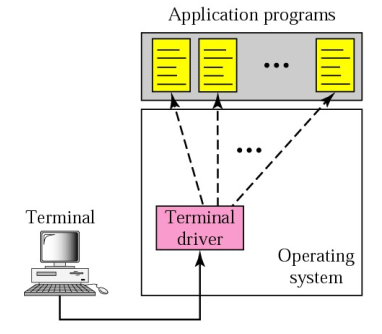
\includegraphics[scale=0.5]{locallogin.png}\\
In \textbf{Local Login} il S.O. assume che gli input ad un processo vengano forniti dallo standard input (tastiera) e che gli output siano inviati allo standard output (monitor).
\end{multicols}
\pagebreak
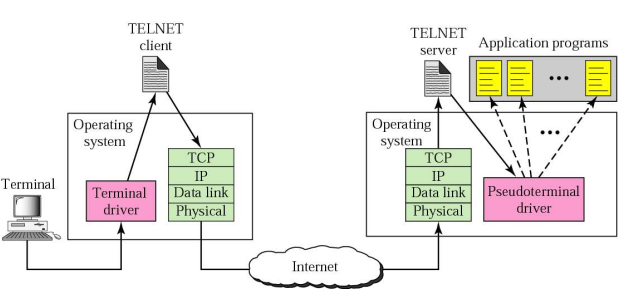
\includegraphics[scale=0.75]{remotelogin.png}\\
In \textbf{Remote Login} lo \textbf{Pseudo Terminal Driver} è l'entry point del S.O. che consente di trasferire caratteri ad un processo \textbf{come se provenissero dal terminale}. Ha il compito di \textbf{accettare i caratteri} dal server e \textbf{trasmetteri al S.O} che li consegnerà all'applicazione opportuna.
\subsection{NVT}
Il Telnet deve \textbf{poter operare con il numero massimo di sistem}, quindi gestire \textbf{dettagli di S.O. eterogenei} che possono differire per:
\begin{list}{}{}
\item \textbf{Set di codifica} dei caratteri
\item \textbf{Lunghezza} della linea e della pagina
\item \textbf{Tasti funzione} individuati da diverse sequenze di caratteri (\textbf{escape sequence})\\
Es. diverse combinazioni per interrompere un processo(\texttt{CTR+C}, \texttt{ESC}), caratteri ASCII diversi per la terminazione di righe di testo.
\end{list}
Per risolvere questo problema si definisce \textbf{un ambiente virtuale}. Sulla rete si considera un \textbf{unico terminale standard} e in corrispondenza di ogni stazione di lavoro si effettuano le \textbf{conversioni da terminale locale a terminale virtuale e viceversa}.
\paragraph{Network Virtual Terminal} Telnet assume che sui due host sia in esecuzione un \textbf{Network Virtual Terminal}, la connessione TCP è stabilita tra i due terminali NVT.\\
L'NVT è un dispositivo \textit{immaginario} che \textbf{fornisce una rappresentazione astratta di un terminale canonico}. Gli host, sia client che server, traducono le loro caratteristiche locali così da \textbf{apparire esternamente come un NVT} e assumo che l'host remoto sia un NVT.\\\\
Il Network Virtual Terminal definisce un \textbf{set di caratteri e di comandi} universale, che permette di:
\begin{list}{}{}
\item \textbf{Trasformare il set di caratteri in uso} localmente \textbf{in un set di caratteri universale} (lettere accentate, tasti freccia, backspace\ldots), includendo anche i caratteri di controllo più importanti (break\ldots)
\item \textbf{Inviare i caratteri di controllo in maniera privilegiata} (meccanismo URGENT del TCP)
\end{list}
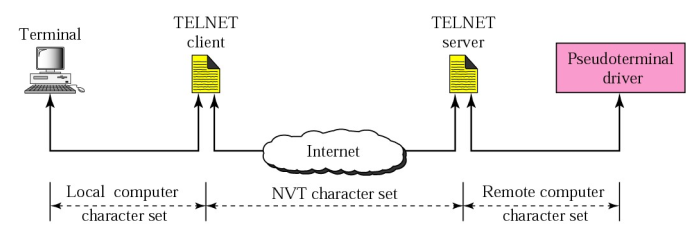
\includegraphics[scale=0.75]{NVT.png}\\
\subsection{Architettura}
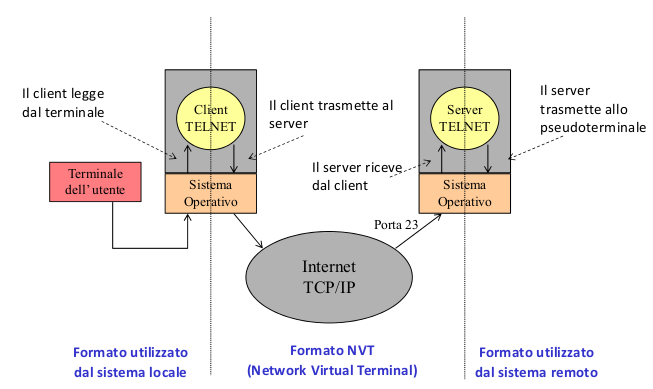
\includegraphics[scale=0.75]{telnetarch.png}
\pagebreak
\subsection{Funzionamento}
Rispetto alla esecuzione in locale, sono aggiunti una \textbf{serie di intermediari}:
\begin{list}{}{}
\item Il client Telnet \textbf{trasforma in NVT} ed usa il S.O. per inviare sulla rete;
\item la rete ed il S.O. server portano i dati al server Telnet;
\item il server Telnet \textbf{traduce da NVT a S.O.} remoto;
\item il S.O. remoto \textbf{esegue} il dovuto;
\item si percorre il cammino inverso con gli stessi soggetti.
\end{list}
Un esempio:
\begin{enumerate}
\item L'utente digita \texttt{INVIO} sulla tastiera
\item Il S.O. passa al client il carattere \texttt{CR}
\item Il client converte \texttt{CR} in \texttt{CR-LF} e lo invia sulla connessione TCP
\item Il server riceve \texttt{CR-LF}, lo converte in \texttt{LF} e lo passa allo pseudoterminale
\item Lo pseudoterminale passa all'applicazione \texttt{LF}
\item L'applicazione esegue l'operazione di \texttt{INVIO}
\end{enumerate}
\paragraph{Formato} I terminali NVT si scambiano i dati in \textbf{formato 7bit US-ASCII}. Ogni carattere è inviato come un ottetto con il primo bit settato a 0. I byte con il bit più significativo a 1 sono usati per le \textbf{sequenze di comandi}.\\
I comandi (es. end-of-line trasmesso come la seuqenza \texttt{CR-LF}) iniziano con un ottetto speciale (\textbf{Interpret as Command} o \texttt{IAC}) di 1 $\rightarrow$ \textbf{Inband Signalling} (comandi e dati sulla stessa connessione).\\\\
I messaggi di controllo iniziali sono usati per scambiare informazioni sulle caratteristiche degli host (\textbf{Telnet  Option Negotiation}).\\
\paragraph{Comandi} Qualche esempio
\begin{center}
\begin{tabular}{c | c c}
\textbf{Comando} & \textbf{Codifica Decimale} & \textbf{Significato} \\
\texttt{IAC} & 255 & Interpreta come comando l'ottetto successivo \\
\texttt{EL} & 248 & Erase Line \\
\texttt{EC} & 247 & Erase Character \\
\texttt{IP} & 244 & Interrupt Process \\
\texttt{EOR} & 239 & End of Record \\
\end{tabular}
\end{center}
\paragraph{NVT conviene?} Suppongo di voler far interoperare N sistemi.\\
Senza usare NVT, ho bisogno di scrivere N-1 client per ogni sistema, e N server (uno per sistema) = \textbf{devo scrivere N(N-1)+N applicazioni}.\\
Usando NVT invece devo scrivere soltanto N server e N client, cioè \textbf{2N applicativi}.\\
Per N $>$ 2 conviene NVT.
\pagebreak
\section{SSH}
Poiché Telnet passa tutto in chiaro, \textbf{anche le password}, con il tempo si è resa necessaria una maggiore sicurezza.
\paragraph{Secure Shell} SSH è un'applicazione nata per \textbf{sostituire Telnet} e \textbf{risolvere i suoi problemi di sicurezza}. Facilita la comunicazione sicura tra client e server e permette la login remota, resa sicura attraverso \textbf{tecniche di cifratura}. Nella realtà SSH offre \textbf{funzionalità molto superiori} a quelle di Telnet\footnote{Vedi su Forouzan}.
\begin{multicols}{2}
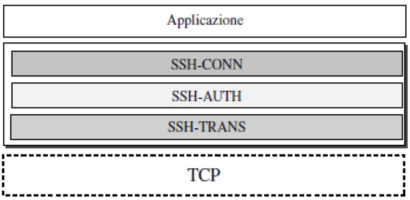
\includegraphics[scale=0.55]{stackssh.png}\\
\columnbreak

\paragraph{SSH-TRANSPORT} Realizza la \textbf{connessione sicura} tra due host:
\begin{list}{}{}
\item Autenticazione del server
\item Negoziazione degli algoritmi di cifratura
\item Scambio di chiavi
\end{list}
\paragraph{SSH-AUTHENTICATION} Meccanismi per autenticare l'utente
\paragraph{SSH-CONNECTION} Sessioen di login remoto, tunneling
\end{multicols}
\section{TCP Port Forwarding}
\paragraph{Port Forwarding} L'inoltro delle porte è un meccanismo che permette di creare un \textbf{canale di comunicazione sicuro} attraverso il quale veicolare qualsiasi tipo di connessione TCP.\\
Viene \textbf{creato un canale di comunicazione cifrato tra la porta all'indirizzo remoto} al quale ci si vuole collegare \textbf{ed una porta locale libera}. In questo modo le applicazioni punteranno il collegamento alla porta locale e la connessione verrà \textbf{inoltrata automaticamente} all'host remoto tramite un canale sicuro.\\
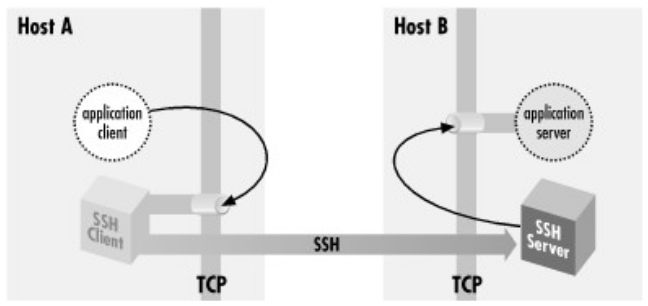
\includegraphics[scale=0.75]{portforwarding.png}\\\\
\texttt{ssh -L 123:localhost:456 remotehost}

\texttt{-L} specifica che la data porta sull'host locale è da 

inoltrare alal data porta sull'host remoto.\\

\texttt{<porta locale>:<host>:<porta remota di host>}
\pagebreak
\section{FTP}
Il \textbf{File Transfer Protocol} (\texttt{RFC 959}) è usato per il \textbf{trasferimento di file da/a un host remoto}. Segue il modello client server:
\begin{list}{}{}
\item Client: il lato che \textbf{chiede} il trasferimento
\item Server: l'host remoto
\end{list}
\paragraph{Standard} Nelle reti TCP/IP lo FTP è lo \textbf{standard per il trasferimento di file}. Questo è un servizio \textbf{diverso} dall'accesso condiviso online (che è un \textbf{accesso simultaneo} da parte di più programmi \textbf{ad un singolo file}).\\
\begin{list}{}{L'FTP fornisce anche \textbf{funzionalità aggiuntive} oltre al semplice trasferimento di file:}
\item \textbf{Accesso interattivo}: l'utente può \textbf{navigare} e \textbf{cambiare/modificare} l'albero di directory nel file system remoto
\item \textbf{Specifica del formato} dei dati da trasferire (es. file di testo o file binari)
\item \textbf{Autenticazione}: il client può specificare username e password
\end{list}
\subsection{Modello FTP}
\begin{list}{}{L'FTP ha \textbf{due tipi di connessione}:}
\item \textbf{Control connection}: scambio di comandi e risposte tra client e server, segue il protocollo Telnet
\item \textbf{Data connection}: connessione su cui i dati sono trasferiti con modi e tipi specificati. I dati trasferiti possono essere \textbf{parte} di file, \textbf{un} file o \textbf{un set} di file.
\end{list}
\subsubsection{Connessione di Controllo}
Il client FTP \textbf{contatta il server FTP alla porta 21} usando il TCP come protocollo di trasporto. Il client \textbf{ottiene l'autorizzazione} sulla connessione di controllo (es. cambio directory, invio file ecc\ldots).\\
La \textbf{connessione} è \textbf{persistente}.
\subsubsection{Connessione Dati}
Quando il server riceve un comando per trasferire file (da o verso il client), \textbf{apre una connessione TCP} con il client.\\ \textbf{Active Mode}: una connessione per ciascun trasferimento e dopo il trasferimento di un file il server chiude la connessione.\\\\
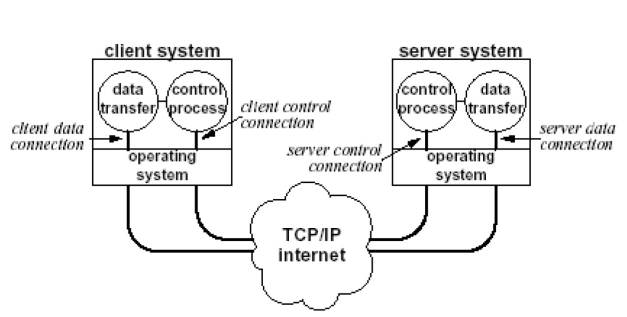
\includegraphics[scale=0.75]{modelloftp.png}
\pagebreak
\subsection{Altri Dettagli}
\begin{list}{}{}
\item Quando un client attiva la connessione di controllo con il server usa un \textbf{numero di porta assegnato localmente in modo casuale} e contatta il server ad una porta nota, cioè la 21
\item FTP usa la connessione di controllo per permettere a client e server di \textbf{coordinare l'uso delle porte assegnate dinamicamente} per il trasferimento dati
\item La \textbf{connessione di controllo} FTP \textbf{si basa sul protocollo Telnet}
\item \subsubsection{Due Modalità} Per creare la connessione TCP per il trasferimento dati sono possibili due modalità:
\begin{list}{}{}
\item \textbf{Active Mode}: vedi sopra, una connessione per ciascun trasferimento e dopo il trasferimento di un file il server chiude la connessione. Il server deve conoscere il numero di porta lato client (glielo comunica)
\item \textbf{Passive Mode}: il \textbf{client ottiene un numero di porta dal server} (porta 20, non necessariamente).\\
Il server non deve accettare connessioni da un processo arbitrario.\\\
Da \texttt{RFC 959} -- PASV: questo comando richede che il server-DTP "ascolti" su una porta dati (che non è quella predefinita) e di aspettare una connessione piuttosto che iniziarne una alla ricezione del comando di trasferimento. La risposta a questo comando include l'host e l'indirizzo e porta su cui il server sta ascoltando.
\end{list}
\end{list}
\textbf{DTP}: Data Transfer Process\\
\textbf{PI}: Protocol Interpreter\\
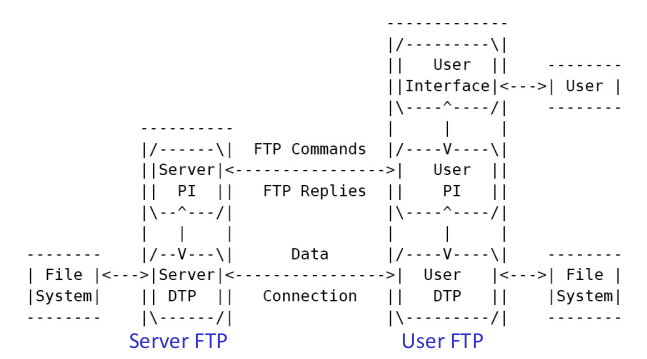
\includegraphics[scale=0.75]{modelloftp2.png}
\begin{list}{}{}
\item \textbf{I dispositivi} dove risiedono client e server FTP \textbf{sono diversi}: S.O., diverse strutture per gestire i file, diversi formati dei file\ldots
\item Per effettuare il trasferimento di file, il client deve \textbf{definire il tipo di file}, la \textbf{struttura dati} e la \textbf{modalità di trasmissione} al fine di risolvere i problemi di eterogeneità tra client e server.
\item Il \textbf{trasferimento file} viene \textbf{preparato attraverso uno scambio di informazioni lungo la connessione di controllo}
\item La \textbf{comunicazione} sulla connessione di controllo \textbf{avviene per mezzo di caratteri con una codifica standard NVT ASCII}, sia per i comandi che per le risposte
\item \subsubsection{Stateful} \textbf{FTP è un protocollo stateful}. Il server deve \textbf{tenere traccia dello stato} dell'utente: tra le altre cose anche della connessione di controllo associata ad un account e della directory attuale.
\item \subsubsection{Modalità di trasmissione}
\begin{list}{}{}
\item \textbf{Stream mode}: FTP invia i dati a TCP con un \textbf{flusso continuo di bit}
\item \textbf{Block mode}: FTP invia i dati a TCP \textbf{suddivisi in blocchi}, ognuno dei quali \textbf{preceduto da un header}
\item \textbf{Compressed mode}: si trasmette il \textbf{file compresso}
\end{list}
\end{list}
\subsection*{Comandi di Controllo}
\begin{list}{}{}
\item \texttt{USER username}
\item \texttt{PASS password}
\item \texttt{LIST}, elenca i file della directory corrente
\item \texttt{NLST}, richiede l'elenco di file e directory (\texttt{ls})
\item \texttt{RETR filename}, recupera (\texttt{get}) un file dalla directory corrente
\item \texttt{STOR filename}, memorizza (\texttt{put}) un file nell'host remoto
\item \texttt{ABOR}, interrompe l'ultimo comando ed i trasferimenti in corso
\item \texttt{PORT}, indirizzo e numero di porta del client
\item \texttt{SYST}, il server restituisce il tipo di sistema
\item \texttt{QUIT}, chiude la connessione
\end{list}
\subsection*{Codici di Ritorno}
I codici di ritorno sono composti da un codice di stato e da un'espressione, come in HTTP:
\begin{list}{}{}
\item \texttt{331 Username OK, password required}
\item \texttt{425 Can't open data connection}
\item \texttt{452 Error writing file}
\item \texttt{200 Comando OK}
\item \texttt{125 Data connection already open, transfer starting}
\item \texttt{225 Data connection open}
\item \texttt{225 Closing data connection. Requested file action succesful} (es. trasferimento file o \texttt{ABOR})
\item \texttt{426 Connection closed, transfer aborted}
\item \texttt{227 Entering passive mode}
\end{list}
\subsection{Anonymous FTP} Server che supportano connessioni FTP senza autenticazione, spesso consentendo operazioni limitate.\\
\texttt{ftp.ed.ac.uk}, user: \texttt{ftp} e password la mail.
\pagebreak
\section{DNS}
\paragraph{Identificare il processo} Ogni processo di livello applicativo ha necessità di \textbf{individuare il processo omologo} con il quale vuole comunicare. Il processo omologo \textbf{risiede su una} particolare \textbf{macchina remota anch'essa da indivudare} (sappiamo che usa lo stesso protocollo).
\subparagraph{Nome} Uno \textbf{nome identifica un oggetto}. Consiste in una sequenza di caratteri scelti da un alfabeto finito, scelta per scopo mnemonico.\\
Nome significativo di alto livello (alfanumerico), vero e proprio identificativo di livello applicativo.
\subparagraph{Indirizzo} Un \textbf{indirizzo identifica dove tale oggetto è situato}.\\
Host di internet usano indirizzi IP (32bit) per instradare i datagrammi (livello di rete). Il formato è scelto per garantire l'efficienza dell'instradamento.\\
\textbf{Disaccoppiamento}: ad un nome possono essere associati più indirizzi.\\\\
\textbf{Come associare indirizzo IP e nome?}
\subsection{Motivazioni}
\paragraph{Inizi} All'inizio l'associazione fra nomi logici e indirizzi IP era \textbf{statica}: tutti i nomi logici ed i relativi indirizzi erano contenuti in un file (\textbf{host file}) periodicamente aggiornato da un server ufficiale. Questo approccio è infattibile nella rete internet attuale:
\begin{list}{}{}
\item Non è possibile che \textbf{ogni host mantenga una copia aggiornata} dell'elenco. Questo per dimensioni dell'elenco, per i volumi di traffico per trasferire i cambiamenti\ldots
\item Non è possibile \textbf{centralizzare un elenco del genere}: si avrebbe così un unico punto di fallimento, un gigantesco volume di traffico sul server\ldots\\
Questa soluzione non è scalabile.
\end{list}
Per questo si utilizza il \textbf{Domain Name System}
\subsection{Struttura}
Il DNS è \textbf{posizionato nel livello applicativo}: gira sui terminali a paradigma client-server. Si affida al sottostante protocollo di trasporto punto-punto per trasferire i messaggi tra i terminali.
\begin{list}{}{}
\item \textbf{Non interagisce direttamente con utenti}
\item La \textbf{complessità} è \textbf{spostata alle estremità} della rete
\end{list}
\begin{multicols}{2}
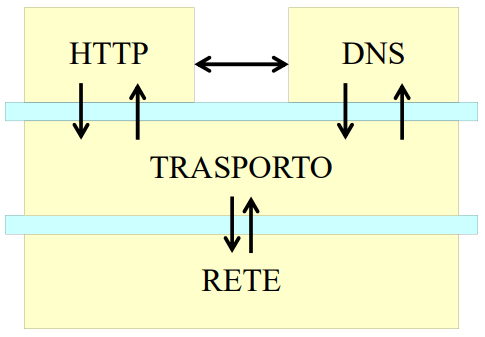
\includegraphics[scale=0.7]{schemadns.png}
\columnbreak

Il DNS è un meccanismo che deve:
\begin{list}{}{}
\item \textbf{Specificare la sintassi} dei nomi \textbf{e le regole} per gestirli
\item \textbf{Consentire la conversione} nomi $\rightarrow$ indirizzi e viceversa
\end{list}

Il DNS è costituito essenzialmente da:
\begin{list}{}{}
\item \textbf{Schema di assegnazione dei nomi}, gerarchico e basato su domini
\item \textbf{Database distribuito} contenente i \textbf{nomi} e le \textbf{corrispondenze} con gli indirizzi
\item \textbf{Protocollo per la distribuzione} delle informazioni sui nomi \textbf{tra i vari name server}
\end{list}
\end{multicols}
\pagebreak
\subsection{Servizi}
I servizi offerti dal DNS sono molteplici:
\begin{list}{}{}
\item \textbf{Risoluzione} di nomi di alto livello (\textbf{hostname}) in indirizzi IP
\item \textbf{Host aliasing}: un host può avere più nomi, solitamente il nome canonico + sinonimi.\\
Es. \texttt{realy1.west-coast.enterprise} può avere due alias \texttt{enterprise.com} e \texttt{www.enterprise.com}.
\item \textbf{Mail Server aliasing}: ci possono essere domain name identici per mail server e web server
\item \textbf{Distribuzione del carico} tra vari server replicati.\\
Ad un hostname canonico possono corrispondere diversi indirizzi IP. La lista di indirizzi viene ordinata in modo diverso in ogni risposta alla richiesta di risoluzione del nome, così che ogni server replicato possa essere scelto con uguale probabilità, distribuendo così efficientemente le richieste.
\end{list}
\subsection{Spazio dei nomi}
Dato che internet è una rete di proporzioni enormi, si presentano i problemi di \textbf{identificazione delle macchine} e \textbf{instradamento dei pacchetti}. si adotta un \textbf{approccio stratificato} poiché è un sistema complesso.\\
\subsubsection{Indirizzi} In internet esistono più indirizzi
\begin{list}{}{}
\item Indirizzi \textbf{MAC}, quello della scheda di rete.\\Solitamente prefissato
\item Indirizzo \textbf{di rete} (\textbf{IP})\\Es. \texttt{150.217.8.21}\\Assegnato dal gestore di rete in base al tipo di rete a cui si appartiene (classe di sottorete)
\item Indirizzo \textbf{di trasporto}\\Coppia $<$\texttt{indirizzo IP}, \texttt{porta}$>$\\La porta è scelta a livello applicativo con regole appropriate
\item Indirizzo \textbf{alfanumerico}\\Es \texttt{medialab.det.unifi.it}\\Libero, basta che sia mappato in un NameServer
\end{list}
\subsubsection{Nomi}
Lo \textbf{spazio dei nomi} deve permettere di \textbf{identificare in modo univoco} un host.
\begin{list}{}{}
\item \textbf{Struttura flat}: sequenza di caratteri senza alcuna ulteriore struttura. Poco applicabile.
\item \textbf{Struttura gerarchica}: un nome è \textbf{costituito da diverse parti}.\\Requisiti per la partizione dello spazio dei nomi:
\begin{list}{}{}
\item \textbf{Conversione efficiente}
\item \textbf{Controllo decentralizzato} dell'assegnazione dei nomi.\\Delega dell'autorità per le varie parti dello spazio dei nomi e \textbf{distribuzione della responsabilità} della conversione tra nomi e indirizzi
\end{list}
Vantaggi e svantaggi
\begin{list}{}{}
\item -- Minore velocità
\item + Maggiore flessibilità
\item + Riconfigurazione più veloce
\item + Possibilità di aggiornamenti decentrati
\end{list}
\end{list}
\pagebreak
\paragraph{Nomi di dominio} Spazio dei nomi con \textbf{struttura gerarchica}. I nomi hanno una \textbf{struttura ad albero} con un numero di livelli variabile. \textbf{Ogni nodo definisce un livello gerarchico} ed è individuato da un'\textbf{etichetta} (max 63 caratteri). Alla radice è associata un'etichetta vuota.\\
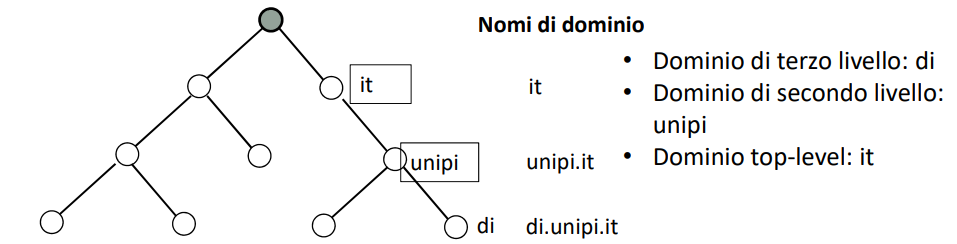
\includegraphics[scale=0.7]{nomidominio.png}\\
Ogni nodo dell'albero ha un nome di dominio, ovvero una \textbf{sequenza di etichette separate da punti} ovvero il cammino foglia $\rightarrow$ radice.
\subparagraph{Dominio} Sottoalbero nello spazio di nomi di dominio che viene identificato dal nome di dominio del nodo in cima al sottoalbero.\\Può essere suddiviso in ulteriori domini, detti \textbf{sottodomini}.
\paragraph{In Internet} Su internet i nomi gerarchici delle macchine sono \textbf{assegnati in base alla struttura delle organizzazioni} che ottengono l'autorità per porzioni dello spazio dei nomi. La struttura gerarchica permette \textbf{autonomia nella scelta dei nomi all'interno di un dominio} perché l'univocità è comunque garantita.\\
Ad es. \texttt{\textbf{server1}.di.unipi.it} e \texttt{\textbf{server1}.cs.cornell.edu} sono due nomi diversi.\\\\
Internet è divisa in \textbf{diverse centinaia di domini} ognuno dei quali \textbf{partizionato in sottodomini} e così via.
\begin{center}
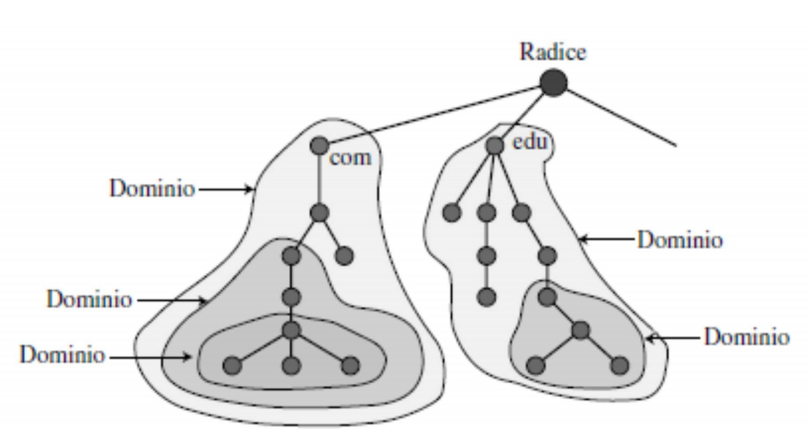
\includegraphics[scale=0.7]{domini.png}
\end{center}
\pagebreak
\subsubsection{Top-Level Domains}
\textbf{Internet Assigned Number Authority} IANA -- \texttt{iana.org}
\begin{list}{}{}
\item \texttt{com} Organizzazioni commerciali
\item \texttt{edu} Istituti d'istruzione (università, scuole\ldots)
\item \texttt{mil} Gruppi militari
\item \texttt{gov} Istituzioni governative
\item \texttt{net} Principali centri di supporto alla rete
\item \texttt{org} Organizzazioni diverse dalle precedenti
\item Codici geografici, schema geografico per nazioni\\Es. \texttt{ir}, \texttt{uk}, \texttt{us}, \texttt{fr}\ldots
\end{list}
\begin{center}
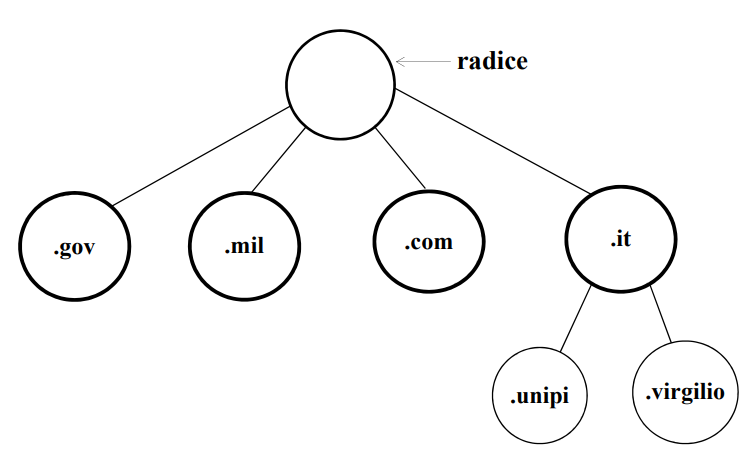
\includegraphics[scale=0.7]{gerarchianomidominio.png}
\end{center}
\subsubsection{Struttura di un nome alfanumerico}
\begin{center}
\texttt{mmedia5.di.unipi.it}
\end{center}
\begin{list}{}{}
\item \texttt{mmedia5} nome locale della macchina (etichetta \textbf{più specifica})
\item \texttt{di.unipi.it} nome del dominio (\texttt{.it} è l'etichetta \textbf{meno specifica})
\item La parte dominio \textbf{può essere ulteriormente suddivisa}, creando così una \textbf{struttura logica gerarchica}\\(\texttt{di} nome locale, \texttt{unipi.it} dominio e così via\ldots)
\end{list}
\pagebreak
\subsection{Conversione}
\paragraph{Indirizzi IP} Gli indirizzi IP sono \textbf{interi a 32bit}. Vengono rappresentati nella \textbf{Decimal Dotted Notation} che divide l'indirizzo IP in 4 \textbf{ottetti}, ovvero 4 gruppi di 8bit. Ad es. \texttt{150.217.8.21}.
\subparagraph{Gerarchia} L'indirizzo IP è strutturato in una gerarchia a due soli livelli.
\paragraph{Indirizzi alfanumerici} Gli indirizzi alfanumerici sono del tipo "\texttt{medialab.di.unipi.it}", sono \textbf{logici}, \textbf{gerarchici} e \textbf{NON indicano in assoluto la locazione geografica} di un host.\\
Vengono \textbf{convertiti da un Domain Name Server in un indirizzo IP}, eventualmente usando un sistema ricorsivo di ricerca.
\paragraph{Database DNS} Il database DNS è \textbf{distribuito} ed implementato in una gerarchia di più name servers.
\paragraph{Protocollo} Il protocollo per la \textbf{risoluzione dei nomi alfanumberici in indirizzi IP} è dello \textbf{strato applicativo}.
\subparagraph{NB} Una funzione fondamentale di internet è implementata come protocollo dello strato applicazione $\rightarrow$ una parte della complessità della rete è \textbf{gestita alle estremità} della rete stessa.
\subsubsection{Name Servers}
Un \textbf{Name Server} è un \textbf{programma che gestisce la conversione da nome di dominio ad indirizzo IP}. I Name Server sono strutturati gerarchicamente.
\begin{center}
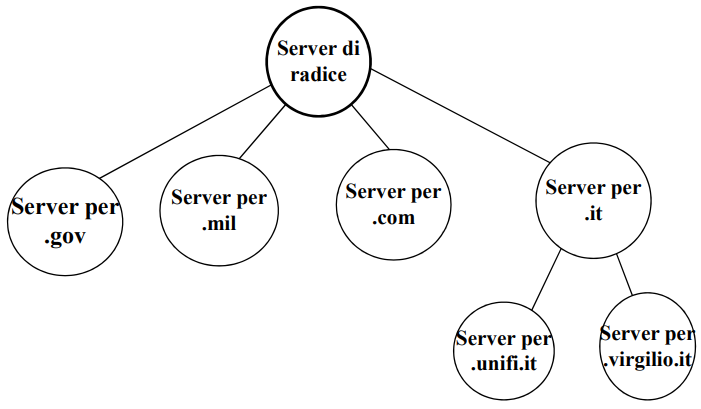
\includegraphics[scale=0.75]{strutturanameservers.png}
\end{center}
Spesso i DNS sono \textbf{accorpati} e \textbf{duplicati} (\textbf{sicurezza}). Inoltre per diminuire il traffico di rete ed il carico dei DNS, ogni server usa \textbf{una cache per le ultime richieste espletate}.
\begin{multicols}{2}
\paragraph{Informazioni} Le informazioni sui domini sono ripartite su più server
\paragraph{Zona} Una zona è una \textbf{regione di cui è responsabile un name server}, tipicamente una parte contigua dell'albero. Zona e dominio non necessariamente coincidono.\\
Il server \textbf{immagazzina le informazioni relative alla propria zona}, inclusi i riferimenti ai server dei domini di livello inferiore.
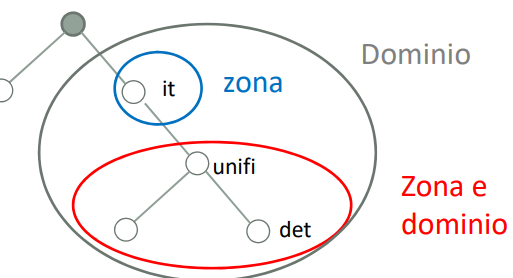
\includegraphics[scale=0.7]{zonadominio.png}
\end{multicols}
\pagebreak
\subsubsection{Root Name Servers}
I \textbf{root name servers} vengono conttatati dai \textbf{local name servers} che non possono risolvere un determinato nome.
\begin{list}{}{Il root name server:}
\item Contatta gli \textbf{authoritative name server} se quella traduzione non è nota
\item \textbf{Recupera la traduzione}
\item \textbf{Invia la traduzione} al local name server
\end{list}
Ce ne sono centinaia in tutto il mondo.\\\\
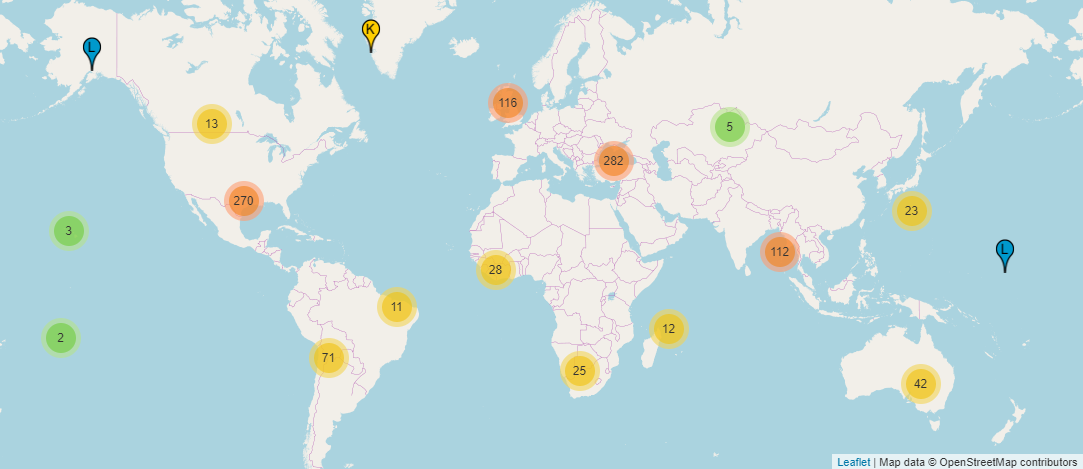
\includegraphics[scale=0.65]{rootns.png}\\
\texttt{root-servers.org}\\
\subsubsection{Gerarchia dei server}
\begin{list}{}{}
\item \textbf{Root Name Server}, server radice
\item \textbf{Top-Level Domain Server}: si occupano dei domini .com, .org, .edu\ldots\\
Ad es. Network Solution gestisce i TLD server per il dominio .com
\item \textbf{Authoritative Name Server}, server di competenza\\
Per un host archivia l'indirizzo IP di quello stesso host. Capace di risolvere la traduzione name/address per quell'hostname.\\
Ogni organizzazione dotata di host internet pubblicamente accessibili (es. web server, server di posta) deve \textbf{fornire i record DNS di pubblico dominio} che mappano i nomi di tali host in indirizzi IP (server mantenuti dall'organizzazione o ISP).
\item Per una certa zona ci possono essere \textbf{server primari} e \textbf{secondari}.
\begin{list}{}{}
\item \textbf{Server primari} mantengono il file di zona
\item \textbf{Server secondari} ricevono il file di zona e offrono il servizio di traduzione
\end{list}
\item \textbf{Local Name Server}\\
Non appartengono strettamente alla gerarchia dei server. Ogni ISP (Università, Società, ISP) ha il \textbf{proprio (default) name server locale}. Le query DNS passano prima dal name server locale.
\end{list}
\pagebreak
\subsection{Risoluzione dei nomi}
Esempio: il client vuole l'IP di \texttt{www.amazon.com}. Prima approssimazione:
\begin{list}{}{}
\item Client \textbf{interroga il server radice} per trovare il server DNS \texttt{com}
\item Client \textbf{interroga il server DNS \texttt{com}} per ottenere il server DNS \texttt{amazon.com}
\item Client \textbf{interrga il server DNS \texttt{amazon.com}} per ottenere l'indirizzo IP di \texttt{www.amazon.com}
\end{list}

\textbf{Query Ricorsiva}\\
Host \texttt{www.tintin.fr} cerca l'IP di \texttt{www.topolino.it}.
\begin{list}{}{}
\item Contatta il suo DNS locale \texttt{dns.tintin.fr}
\item \texttt{dns.tintin.fr} contatta il root name server se necessario
\item Il root name server contatta l'authoritative name server \texttt{dns.topolino.it} se è necessario
\end{list}
Il local name server ha richiesto una conversione completa\\\\
\textbf{Query Iterativa} Le risposte vengono restituite direttamente al client, cioè i name server rispondono con il riferimento al name server da contattare.\\
\begin{multicols}{2}
\textbf{Query Iterativa}\\
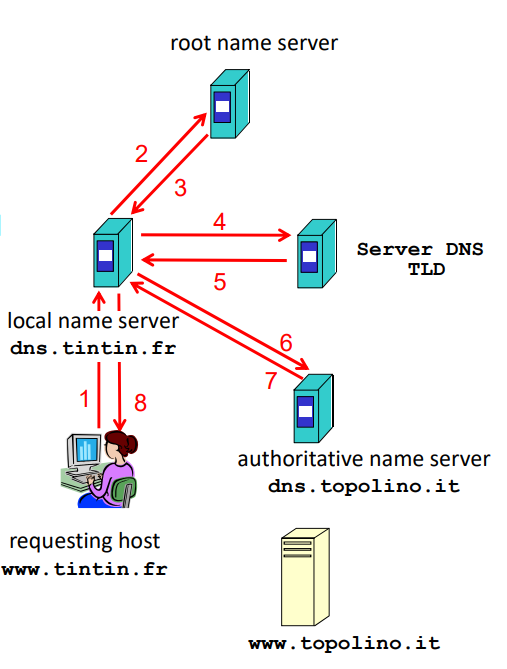
\includegraphics[scale=0.6]{dnsqueryiterativa.png}\\\\\\\\\\



\textbf{Query Ricorsiva}\\
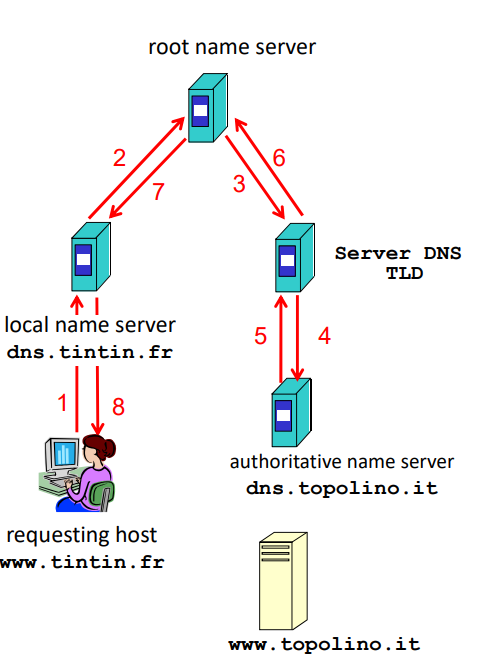
\includegraphics[scale=0.7]{dnsqueryricorsiva.png}
\end{multicols}
\pagebreak
\subsection{Caching e Aggiornamento Record}
Una volta che un name server ha appreso un'associazione, la mette nella \textbf{cache}. \textbf{I record} nella cache vengono \textbf{cancellati dopo un certo tempo} (timeout, TTL). L'utilizzo della cache \textbf{migliora il ritardo} e \textbf{riduce il numero di messaggi DNS}.\\
I meccanismi di update/notifica sono descritti nella \texttt{RFC 2136}.
\subsection{Record DNS}
Il DNS è un \textbf{database distribuito di "resource records"} (\textbf{RR}).
\begin{center}
Formato RR: \texttt{(name, value, type, TTL)}
\end{center}
\begin{list}{}{}
\item \textbf{TTL}: quando la risorsa dovrà essere rimossa dalla cache
\item I significati di \textbf{name} e \textbf{value} dipendono da \textbf{type}
\begin{list}{}{}
\item type = A\\name = hostname\\value = indirizzo IP
\item type = CNAME\\name = hostname (sinonimo)\\value = nome canonico dell'host
\item type = NS\\name = dominio (es. \texttt{unifi.it})\\value = hostname dell'authoritative name server per quel dominio
\item type = MX\\name = nome di dominio\\value = nome canonico del server di posta associato a name
\item Ci sono altri type\ldots
\end{list}
\end{list}
\begin{list}{}{Esempi di record DNS}
\item \texttt{(hostname, indirizzoip, A, \ldots)}\\
\texttt{(www.cnn.com, 157.166.224.25, A, \ldots)}\\
\texttt{(www.cnn.com, 157.166.224.26, A, \ldots)}
\item \texttt{(dominio, nomeDiAuthoritativeServerPerDominio, NS, \ldots)}\\
\texttt{(cli.di.unipi.it, nameserver.cli.di.unipi.it*, NS, \ldots)}\\
$[$* ANSWER conterrà anche \texttt{(nameserver.cli.di.unipi.it, 131.114.120.2,A, \ldots)}$]$
\item \texttt{(alias, hostnameMailServerConTaleAlias, MX, \ldots)}\\
\texttt{(cli.di.unipi.it, mailserver.cli.di.unipi.it*, MX, \ldots)}\\
$[$* ANSWER conterrà anche \texttt{(mailserver.cli.di.unipi.it, 131.114.11.39, A, \ldots)}$]$
\end{list}
\subsection{Messaggi DNS}
Query e risposte hanno lo \textbf{stesso formato}.\\
Le query contengono \textbf{QName} e \textbf{QType} nella sezione "\textbf{question}".\\
Le risposte contengono 0 o più RR nella sezione "\textbf{answer}" e 0 o più RR nella sezione "\textbf{additional}".\\
Per esempio:
\begin{list}{}{}
\item \texttt{dns.poly.edu} $\longrightarrow$ TLD server\\
Question: QName=\texttt{gaia.cs.mass.edu} QType=A
\item \texttt{dns.poly.edu} $\longleftarrow$ TLD server\\
Answer: \texttt{(umass.edu, dns.umass.edu, NS)}\\
Additional: \texttt{(dns.umass.edu, 128.115.40.41, A)}
\end{list}
\pagebreak
\begin{multicols}{2}
\textbf{Header} dei messaggi DNS
\begin{list}{}{}
\item \textbf{Identification}: 16 bit. Identification usato dalle query, la reply ad una query usa lo stesso identification.
\item \textbf{Flags}
\begin{list}{}{}
\item Query (0) o reply (1)
\item Recursion desired
\item Recursion available
\item Reply is authoritative
\end{list}
\end{list}
Il protocollo DNS usa tipicamente \textbf{UDP sulla porta 53 per le query DNS} (dimensioni del messaggio inferiori a 512B). Possibile usare TCP, ad esempio per trasferire i dati tra DNS server -- Zone Transfers)


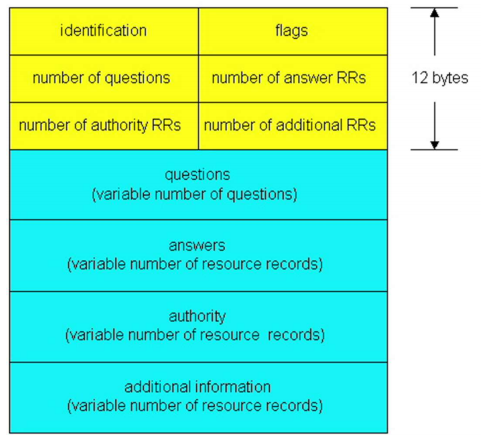
\includegraphics[scale=0.7]{dnsmsgheader.png}
\end{multicols}
\begin{list}{}{}
\item \textbf{Domande}: campi per il nome richiesto ed il tipo di domanda
\item \textbf{Risposte}: RR nella risposta della domanda
\item \textbf{Competenza}: record per i server di competenza
\item Informazioni aggiuntive
\end{list}
\begin{multicols}{2}
\textbf{Questions}\\
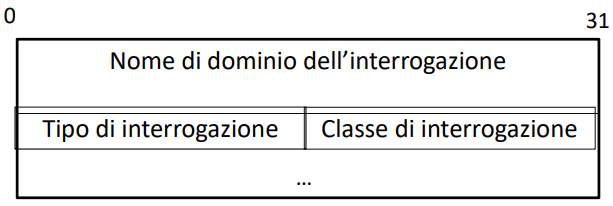
\includegraphics[scale=0.5]{dnsquestions.png}
\columnbreak
\begin{list}{}{}
\item \textbf{Tipo di Interrogazione}: tipo di domanda (nome di una macchina o indirizzo di posta)
\item Il \textbf{client} riempie la sezione di \textbf{domanda}
\item Il \textbf{server}, nel proprio messaggio di \textbf{risposta}:
\begin{list}{}{}
\item \textbf{ricopia la} sezione di \textbf{domanda}
\item \textbf{riempie le altre sezioni} (risposta, autorità, altre info) con RR
\end{list}
\end{list}
\end{multicols}
\textbf{Le RFC di riferimento} sono:
\begin{list}{}{}
\item \texttt{RFC 1034: DOMAIN NAMES - CONCEPTS AND FACILITIES}\\
Definisce i seguenti tipi di record:
\begin{list}{}{}
\item \textbf{A} indirizzo dell'host
\item \textbf{CNAME} nome canonico
\item \textbf{HINFO} CPU e S.O. usato dall'host
\item \textbf{MX} mail exchange
\item \textbf{NS} Authoritative Name Server
\item \textbf{PTR} name space pointer
\item \textbf{SOA} Inizio di una zona d'autorità
\end{list}
\item \texttt{RFC 1035: DOMAIN NAMES - IMPLEMENTATION AND SPECIFICATION}
\end{list}
\pagebreak
\section{SMTP}
\paragraph{Posta Elettronica} Uno dei primi servizi nati su internet è la posta elettronica (1982). Essa consiste nel \textbf{trasferimento di un messaggio tra} uno user \textbf{mittente} e uno user \textbf{destinatario}. Il \textbf{destinatario potrebbe non essere disponibile} in quel momento, e quindi non poter accettare i messaggi: utente impegnato, \textbf{computer spento}.\\\\
Il servizio di posta elettronica si \textbf{basa su componenti intermediari} per trasferire i messaggi: \textbf{disaccoppiamento} lato mittente e destinatario, analogia con posta tradizionale.\\
Il trasferimento di messaggi di posta elettronica si basa sul \textbf{Simple Mail Transfer Protocol} (\texttt{RFC 821}, \texttt{RFC 2821}, \texttt{RFC 5321}).
\paragraph{Componenti principali}
\begin{list}{}{}
\item \textbf{Agenti utente}
\item \textbf{Mail Server}
\item \textbf{Protocolli}
\end{list}
\subsection{Agenti Utente}
Detti anche \textbf{mail reader}, usati per la \textbf{composizione}, editing, \textbf{lettura} di messaggi di posta.
\begin{list}{}{Ad es:}
\item Eudora
\item Outlook
\item Thunderbird
\end{list}
I messaggi in entrata e uscita \textbf{vengono archiviati sul server}
\subsection{Mail Server}
Le \textbf{mailbox} (casella) \textbf{contengono}
\begin{list}{}{}
\item \textbf{i messaggi in ingresso diretti all'utente} ancora da leggere
\item una \textbf{coda di messaggi in uscita} ancora da inviare
\item il \textbf{protocollo SMTP} per il dialogo tra mail server, allo scopo di scambiare i messaggi
\begin{list}{}{}
\item \textbf{Client}: mail server che invia
\item \textbf{Server}: mail server che riceve
\end{list}
\end{list}
Esempio di scenario: Alice invia un messaggio di posta a Bob.
\begin{enumerate}
\item \textbf{Alice}, grazie al suo mail user agent \textbf{compone il messaggio}.\\Alice \textbf{fornisce} allo user agent l'\textbf{indirizzo di destinazione}, cioè l'indirizzo di Bob
\item Lo user agent di Alice \textbf{spedisce il messaggio} al suo server di posta e il messaggio \textbf{viene accodato in attesa di invio}
\item Il \textbf{lato client} dell'SMTP sul server di posta di Alice \textbf{vede il messaggio} e \textbf{apre una connessione al server} SMTP sul server di posta \textbf{di Bob}
\item L'\textbf{SMTP client invia il messaggio nella connessione}
\item Sull'\textbf{host server} di posta di Bob, \textbf{il lato server} dell'SMTP \textbf{riceve il messaggio} e lo \textbf{colloca nella casella di posta di Bob}
\item Bob, \textbf{quando vuole}, \textbf{chiede al suo user agent di leggere il messaggio}
\end{enumerate}
\pagebreak
\subsection{Schema di principio}
\begin{center}
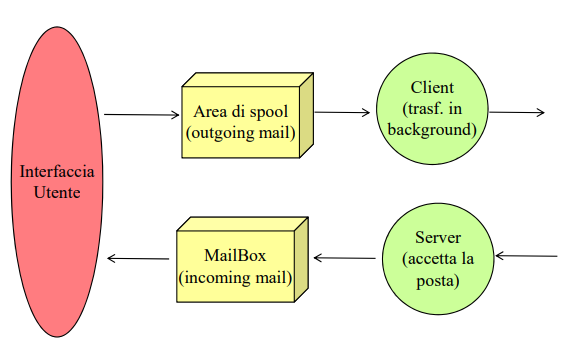
\includegraphics[scale=0.7]{smtpschemascambio.png}
\end{center}
La tecnica adottata dai server di posta si chiama \textbf{spooling}.
\begin{list}{}{}
\item L'utente invia un messaggio, il sistema ne pone una copia in memoria spool -- o \textbf{area di accomodamento della posta}, insieme all'id mittente, id destinatario, id macchina di destinazione e tempo di deposito.
\item Il sistema \textbf{avvia il trasferimento alla macchina remota}. Il sistema (client) stabilisce una connessione TCP con la macchina destinazione.
\item Se la connessione viene aperta, \textbf{inizia il trasferimento del messaggio}
\item Se il trasferimento va a buon fine il \textbf{client cancella la copia locale del film}\\
Se il trasferimento non va a buon fine, il \textbf{processo di trasferimento scandisce periodicamente l'area di spooling} e \textbf{tenta il trasferimento dei messaggi non consegnati}. Oltre un certo intervallo di tempo (definito dall'amministratore del server), se il messaggio non è stato consegnato \textbf{viene inviata una notifica all'utente mittente}.
\end{list}

\subsection{Indirizzo}
Un ricevente è identificato da un indirizzo email del tipo:
\begin{center}
\texttt{local-part @ domain-name}
\end{center}
\begin{list}{}{}
\item \texttt{domain-name}: specifica un \textbf{mail server}. Determina il nome di dominio della destinazione verso la quale la mail deve essere consegnata.\\\textbf{Nome di dominio del server di posta}
\item \texttt{local-part}: specifica una \textbf{casella di posta} sul mail server. Spesso identica al login o al nome completo dell'utente.\\\textbf{Indirizzo della casella di posta del destinatario}
\end{list}
\pagebreak
\subsection{Gestione Alias}
\begin{center}
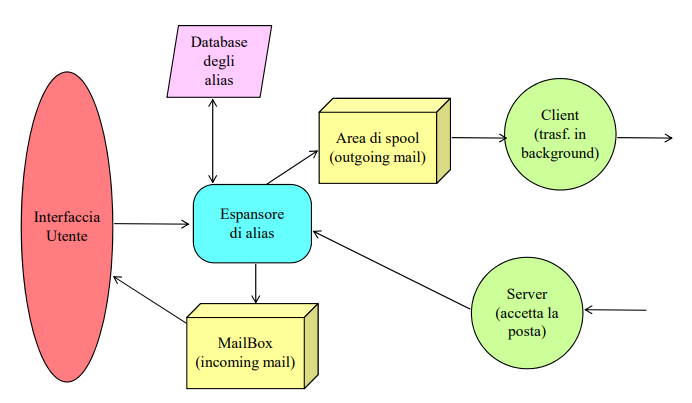
\includegraphics[scale=0.7]{smtpgestalias.png}
\end{center}
L'\textbf{alias} è una \textbf{casella postale virtuale} che serve a \textbf{ridistribuire i messaggi} verso uno o più indirizzi di posta elettronica personali.
\begin{list}{}{}
\item \textbf{Molti -- Uno}: il sistema di alias \textbf{permette ad un signolo utente di avere identificatori di mail multipli}, assegnando un set di identificatori ad una singola persona.\\
Un utente $\longrightarrow$ più indirizzi postali
\item \textbf{Uno -- Molti}: il sistema di alias \textbf{permette di associare un gruppo di destinatari ad un singolo identificatore}.\\
Un indirizzo postale $\longrightarrow$ più utenti destinatari (es. mailing list)
\end{list}
\paragraph{Espansione degli alias postali} \textbf{Conversione di identificatori} di indirizzi postali \textbf{in uno o più indirizzi} postali nuovi.\\
Se l'alias database specifica che all'indirizzo \texttt{x} deve essere assegnato il nuovo indirizzo \texttt{y}, l'espansione dell'alias riscriverà l'indirizzo di destinazione. Si provvederà poi a determinare se \texttt{y} specifichi un indirizzo locale o remoto e lo posizionerà nell'area di spool relativa.
\pagebreak
\subsection{Modello di riferimento}
\begin{center}
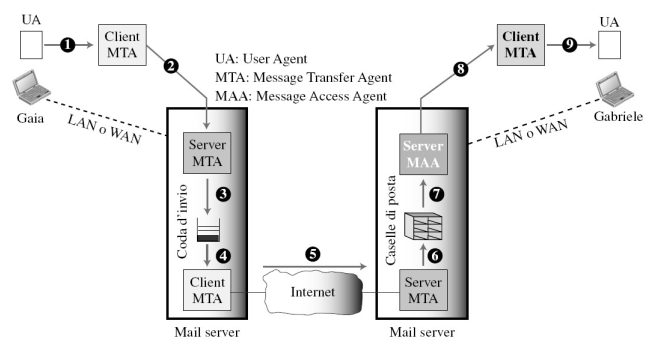
\includegraphics[scale=0.7]{mailmodelloriferimento.png}
\end{center}
\subsection{Simple Mail Transfer Protocol}
\texttt{RFC 821}, \texttt{RFC 2821}, \texttt{RFC 5321}\\
L'obiettivo dell'SMTP è \textbf{trasferire le mail in maniera affidabile ed efficiente}. L'SMTP è \textbf{indipendente dal particolare sottosistema di trasmissione} e \textbf{richiede solo un canale che trasmetta dati ordinati in maniera affidabile}.\\
Nonostante (nelle RFC) si parli specificamente del TCP, altri mezzi di trasporto sono possibili.
\subsection{SMTP Mail Relaying}
Una funzionalità importante dell'SMTP è la capacità di \textbf{trasportare mail attraverso reti multiple}. In questo modo, un messaggio di posta può passare attraverso molti dispositivi intermedi sul suo percorso dal mittente al destinatario.
\begin{center}
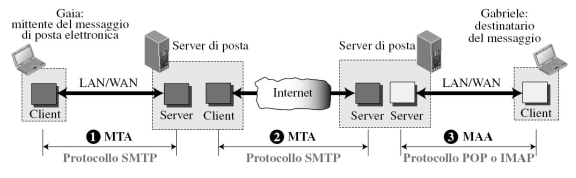
\includegraphics[scale=0.9]{smtpmailrelaying.png}
\end{center}
\pagebreak
\subsection{Modello SMTP}
Quando un client SMTP ha un messaggio da trasmettere, stabilisce una \textbf{canale di trasmissione bidirezionale verso un server SMTP}. La \textbf{responsabilità del client} SMTP è di \textbf{trasferire messaggi di posta a uno o più server SMTP}, o comunicarne il fallimento.
\begin{center}
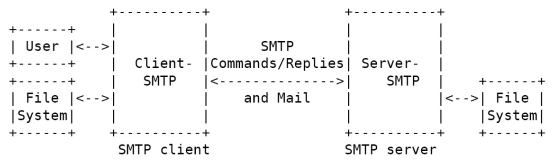
\includegraphics[scale=0.7]{smtpmodello.png}\\
\end{center}
Un client SMTP determina l'indirizzo di un host appropriato che esegue un server SMTP \textbf{risolvendo un nome di dominio di destinazione} ottenendo o un \textbf{mail server intermedio} o l'\textbf{host finale} (tramite query DNS).
\paragraph{Trasferimento} Il trasferimento di un messaggio può avvenire \textbf{in una singola connessione} tra mittente e destinatario o tramite \textbf{una serie di salti tra sistemi intermedi}.\\
In entrambi i casi, una volta che il server ha risposto positivamente alla fine della trasmissione dei dati della mail, avviene una \textbf{cessione di responsabilità del messaggio}: il \textbf{protocollo richiede che un server \textit{debba} accettare la responsabilità di o consegnare} il messaggio \textbf{o segnalare il fallimento} della consegna.
\subsubsection{Fallimenti nella consegna}
\begin{list}{}{Possibili problemi}
\item Connessione con il mail server del mittente\\Server \textbf{inesistente} o \textbf{irraggiungibile}
\item Connessione con il mail server del destinatario\\Server \textbf{insesistente} o \textbf{irraggiungibile}
\item Inserimento nella casella di posta del destinatario\\\textbf{User sconosciuto}, \textbf{casella piena}
\end{list}
In tutti i casi \textbf{il mittente riceve una notifica}!\\
L'unico caso in cui il destinatario non riceve il messaggio e il mittente non viene avvisato è se \textbf{qualcuno rimuove il messaggio} (intrusi, filtri antispam\ldots)
\subsection{Protocollo}
Nella pratica viene usato il \textbf{protocollo TCP} sulla porta 25 per \textbf{consegnare in modo affidabile} i messaggi dal client al server.
\begin{list}{}{Questo avviene in tre fasi:}
\item Handshaking
\item Trasferimento del messaggio
\item Chiusura della connessione
\end{list}
L'\textbf{interazione} avviene tramite \textbf{comando/risposta}, con comandi in testo ASCII e risposte con codici di stato e descrizione facoltativa.\\
I messaggi, header e body, sono in caratteri ASCII a 7bit.
\pagebreak
\begin{multicols}{2}
\paragraph{Protocollo semplice, di comandi e risposte}
I \textbf{comandi e} (a meno di alterazioni dovute ad un estensione del servizio) i \textbf{dati dei messaggi SMTP sono trasmessi} da mittente a destinario \textbf{attraverso il canale di trasmissione in "right"}.\\\\
Una \textbf{risposta SMTP} è un \textbf{riconoscimento} (positivo o negativo) mandato in "righe" da destinatario a mittente attraverso il canale di trasmissione in risposta ad un comando.\\
La forma generale di risposta è un \textbf{codice numerico}, solitamente seguito da una stringa di testo.
\columnbreak
\begin{verbatim}
S: MAIL FROM: <Smith@Alpha.ARPA>
R: 250 OK

S: RCPT TO:<Jones@Beta.ARPA>
R: 250 OK

S: RCPT TO:<Green@Beta.ARPA>
R: 550 No such user here

S: RCPT TO:<Brown@Beta.ARPA>
R: 250 OK

S: DATA
R: 354 Start mail input; end with <CRLF>.<CRLF>
S: Blah blah blah...
S: ...etc. etc. etc.
S: <CRLF>.<CRLF>
R: 250 OK
\end{verbatim}
\end{multicols}
\begin{multicols}{2}
\paragraph{Handshaking}
Il client \textbf{stabilisce la connessione e attende} che il server invii "\texttt{220 READY FOR MAIL}", cioè la disponibilità a ricevere la posta.\\
Il \textbf{client risponde con il comando} \texttt{HELO}\\
Il \textbf{server risponde identificandosi}\\
A questo punto il client può trasmettere i messaggi
\columnbreak
\begin{verbatim}
S: 220 Beta.GOV Simple Mail Transfer Service ready
C: HELO Alfa.EDU
S: 250 Beta.GOV
\end{verbatim}
\end{multicols}
\begin{multicols}{2}
\subsection{Comandi SMTP}
\begin{list}{}{Alcuni comandi:}
\item \texttt{HELO <client identifier>}
\item \texttt{MAIL FROM:<reverse-path> [SP <mail-parameters>] <CRLF>}
\item \texttt{RCPT TO:<forward-path> [SP <rcpt-parameters>] <CRLF>}
\item \texttt{DATA}
\item \texttt{QUIT}
\end{list}
\paragraph{Nota bene} \texttt{<CRLF>.<CRLF>} per terminare la fine di un messaggio
\subsection{Esempio}
\begin{verbatim}
S: MAIL FROM:<Smith@Alpha.ARPA>
R: 250 OK
S: RCPT TO:<Jones@Beta.ARPA>
R: 250 OK
S: RCPT TO:<Green@Beta.ARPA>
R: 550 No such user here
S: RCPT TO:<Brown@Beta.ARPA>
R: 250 OK
S: DATA
R: 354 Start mail input; end with <CRLF>.<CRLF>
S: Blah blah blah...
S: ...etc. etc. etc.
S: <CRLF>.<CRLF>
R: 250 OK
\end{verbatim}
\columnbreak
\textbf{Esempio d'interazione}\\
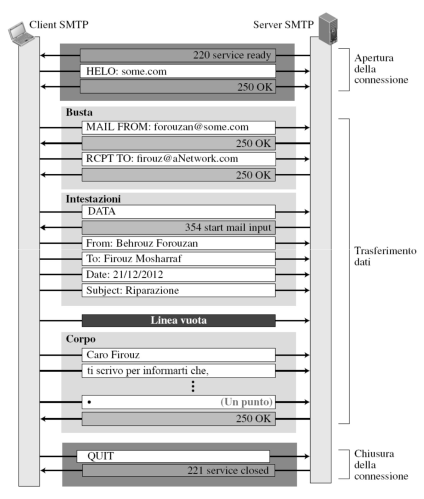
\includegraphics[scale=0.68]{smtpesempio.png}
\end{multicols}
\pagebreak
\subsection{Formato messaggi mail}
L'\textbf{SMTP} è il \textbf{protocollo per lo scambio} dei messaggi\\
L'\texttt{RFC 2822} è lo \textbf{standard formato di testo}:
\begin{list}{}{}
\item \textbf{Linee d'intestazione}
\begin{list}{}{ad esempio}
\item To:
\item From:
\item Subject:
\item \textit{Diversi dai comandi SMTP!}
\end{list}
\item \textit{Linea vuota}
\item \textbf{Body}\\Il "messaggio", solitamente in caratteri ASCII 7bit
\end{list}
\begin{list}{}{Esempi di header:}
\item A.3.1, minimo richiesto
\begin{verbatim}
Date: 26 Aug 76 1429 EDT
From: Jones@Registry.Org
Bcc: 
		-oppure-
Date: 26 Aug 76 1429 EDT
From: Jones@Registry.Org
To: Smith@Registry.Org
\end{verbatim}
Il campo Bcc può essere buoto, il campo \textbf{To deve avere almeno un indirizzo}
\item A.3.2, con qualche campo addizionale
\begin{verbatim}
Date: 26 Aug 76 1430 EDT
From: George Jones<Group@Host>
Sender: Secy@SHOST
To: "Al Neuman"@Mad-Host, Sam.Irving@Other-Host
Message-ID: <some.string@SHOST>
\end{verbatim}
\item A.3.3, il più complesso possibile
\begin{verbatim}
Date    : 27 Aug 76 0932 PDT
From    : Ken Davis <KDavis@This-Host.This-net>
Subjcet : Re: The Syntax in the RFC
Sender  : KSecy@Other-Host
Reply-To: Sam.Irving@Reg.Organization
To      : George Jones <Group@Some-Reg.An-Org>, Al.Neuman@MAD.Publisher
cc      : Important folk:
            Tom Softwood <Balsa@Tree.Root>,
            "Sam Irving"@Other-Host;,
          Standard Distribution:
            /main/davis/people/standard@Other-Host,
            "<Jones>standard.dist.3"@Tops-20-Host>;
Comment : Sam is away on business. He asked me to handle his mail for him. He'll be able to provide
a more accurate explanation when he returns next week.
In-Reply-To: <some.string@DBM.Group>, George's message
X-Special-action: This is a sample of user-defined field-names. There could also be a field-name
"Special-action", but its name might later be preempted
Message-ID: <4231.629.XYzi-What@Other-Host>
\end{verbatim}
\end{list}
% L06_email_SMTP, 26
\pagebreak
\subsection{Estensioni multimediali}
L'\texttt{RFC 822} permette di inviare \textbf{solo messaggi di testo} in ASCII. rice\textbf{Problema: permettere} agli utenti di Internet \textbf{di inviare/ricevere} messaggi
\begin{list}{}{}
\item In \textbf{lingue con accenti} (come l'italiano), in \textbf{alfabeti non latini} (come il russo o l'ebraico) o in \textbf{lingue senza alfabeto} (come il cinese o il giapponese)
\item \textbf{Contenuti audio o video}
\end{list}
\subsubsection{MIME}
\paragraph{Idea di base} \textbf{Continuare ad usare il formato} del messaggio specificato in \texttt{RFC 822} ma \textbf{aggiungendo una struttura al message body} e \textbf{definendo regole di encoding} per il trasferimento di testo non-ASCII.\\
Questo ha permesso di \textbf{inviare messaggi MIME usando protocolli e mail server esistenti}, rendendo però \textbf{necessario cambiare gli user agent}.
\paragraph{Multipurpose Internet Mail Extension} \texttt{RFC 2045} e \texttt{RFC 2046}. Questo standard di Internet \textbf{estende il formato delle mail} per supportare:
\begin{list}{}{}
\item Testo in \textbf{character set diversi} dall'US-ASCII
\item \textbf{Allegati} non di testo
\item Corpo del messaggio diviso in più parti
\item Informazioni nell'header in character set non ASCII
\end{list}
Si realizza con linee di intestazione aggiuntive per dichiarare il tipo di contenuti MIME. La \texttt{RFC 2045} definisce una serie di metodi per rappresentare dati binari in formato ASCII.
\begin{center}
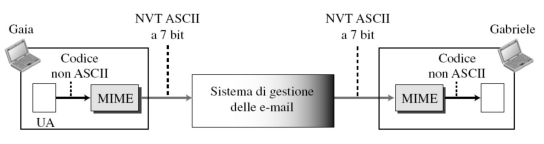
\includegraphics[scale=1]{mime.png}
\end{center}
\begin{verbatim}
From: alice@crepes.fr
To: bob@hamburger.edu
Subject: Picture of yummy crepe.
MIME-Version: 1.0                   \\Versione MIME
Content-Transfer-Encoding: base64   \\Metodo usato per la codifica dei dati
Content-Type: image/jpeg            \\Dati multimediali (tipo, sottotipo, parametri...)

base64 encoded data .....
.........................           \\Dati codificati
......base64 encoded data
\end{verbatim}
\begin{list}{}{Campi nell'header:}
\item \textbf{MIME-Version}: un \textbf{numero di versione} per dichiarare a quale versione aderisce il formato del messaggio
\item \textbf{Content-Type}: usato per \textbf{specificare il tipo del media e il sottotipo dei dati} nel corpo del messaggio, e per specificare completamente la rappresentazione nativa di quei dati
\item \textbf{Content-Transfer-Encoding}: specifica la \textbf{codifica applicata} al corpo del messaggio. La codifica è solitamente applicata ai dati per consentire loro di passare attraverso i meccanismi di trasporto delle mail, che potrebbero avere limitazioni sui dati o sui character set.
\end{list}
La maggior parte dei tipi di media che è utile trasportare via mail sono \textbf{nativamente rappresentati con caratteri di 8bit} o dati binari. I \textbf{client e i server} SMTP si \textbf{aspettano messaggi ASCII} (caratteri a \textbf{7 bit}), i \textbf{dati binari invece usato tutti e 8 bit} del byte (es. immagini, eseguibili, set estesi di caratteri).\\
MIME fornisce \textbf{cinque schemi di transfer encoding} tra cui:
\begin{list}{}{}
\item \textbf{Codifica ASCII} dei dati binari: \textbf{codifica base64}\\
Gruppi di 28bit divisi in 4 unità da 6bit, ciascuna unità inviata come un carattere ASCII
\item \textbf{Quoted-printable encoding}: per messaggi con pochi caratteri non-ASCII, più efficiente
\end{list}
Oggigiorno i mail server possono negoziare l’invio di dati in codifica binario (8 bit), se la negoziazione non ha successo si usano i caratteri ASCII.
\subsubsection{Tipi MIME}
\begin{center}
\texttt{Content-Type: type/subtype; parameters}
\end{center}
\begin{list}{}{}
\item \textbf{Text}\\Esempi di subtype: \texttt{plain}, \texttt{html}
\item \textbf{Image}\\Esempi di subtype: \texttt{jpeg}, \texttt{gif}
\item \textbf{Audio}\\Esempi di subtype: \texttt{basic} (8bit mu-law encoded), \texttt{32kadpcm} (32 kbps)
\item \textbf{Video}\\Esempi di subtype: \texttt{mpeg}
\item \textbf{Application}\\Altri dati che devono essere processati da un'applicazione prima di essere visualizzabili.\\Esempi di subtype: \texttt{msword}, \texttt{octet-stream} (dati arbitrari binari)
\end{list}
\subsection{Protocolli di accesso alla mail}
\begin{center}
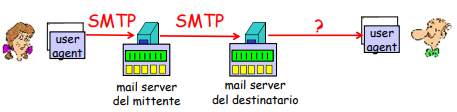
\includegraphics[scale=1]{mailaccesso.png}
\end{center}
Per trasferire la posta fino al server del destinatario si utilizza l'SMTP, che è un protocollo di tipo push: la maggiorparte dei dati è dal client al server. Per \textbf{leggere la posta} invece, è richiesto un protocollo di tipo pull, cioè in cui i dati viaggiano prevalentemente dal server al client.
\paragraph{Messagge Access Agent} Attualmente si utilizzano due protocolli di accesso alla posta
\begin{list}{}{}
\item \textbf{POP}  Post Office Protocol\\Semplice ma con funzionalità limitate. Attualmente è in uso la terza versione, POP3.
\begin{list}{}{}
\item \textbf{Fase di autorizzazione}\\L'accesso avviene con lo \textbf{user agent} che \textbf{apre una connessione TCP sulla porta 110} e si autentica con i comandi
\begin{list}{}{}
\item \texttt{user}: specifica lo username
\item \texttt{pass}: specifica la password
\end{list}
ed il server risponderà con \texttt{OK} o \texttt{ERR}.
\pagebreak
\item \textbf{Fase di transazione}\\Il client può utilizzare i comandi:
\begin{list}{}{}
\item \texttt{list}: visualizza la \textbf{lista dei messaggi}
\item \texttt{retr}: \textbf{preleva il messaggio} per numero
\item \texttt{dele}: \textbf{elimina il messaggio dal server}
\item \texttt{quit}: \textbf{chiude la sessione}
\end{list}
\item \textbf{Fase di aggiornamento}\\Dopo aver ricevuto \texttt{quit} il server cancella i messaggi marcati per la rimozione
\end{list}
Il POP3 ha due modalità:
\begin{list}{}{}
\item \textbf{Delete}: i \textbf{messaggi vengono automaticamente eliminati} dalla mailbox \textbf{dopo il  prelievo}
\item \textbf{Keep}: i \textbf{messaggi vengono conservati dopo il prelievo}
\end{list}
Inoltre non mantiene le informazioni di stato tra le sessioni, solo le cancellazioni sono permesse.
\item \textbf{IMAP}  Internet Mail Access Protocol\\
Ha più funzionalità, ed è più complesso, del POP3. Consente tra le altre cose di \textbf{manipolare i messaggi memorizzati sul server} con cartelle, e di \textbf{estrarre solo alcuni componenti dei messaggi} come solo l'intestazione se si sta usando una connessione lenta.
\item \textbf{HTTP}\\Es. Hotmail, Yahoo! Mail, \ldots
\end{list}
\section{Livello di Trasporto}
\subsection{Obiettivi}
\paragraph{}Realizzare una \textbf{connessione logica fra processi residenti in host diversi}.
\subparagraph{Logico} I processi si comportano \textbf{come se gli host fossero direttamente collegati}, non si preoccupano dei dettagli dell'infrastruttura usata fisica per la comunicazione.
\paragraph{}\textbf{Offrire servizi allo strato applicativo}
\subparagraph{} Un'applicazione \textbf{interagisce con i protocolli di trasprto per trasmettere e ricevere dati}. L'applicazione sceglie lo stile di trasporto: sequenza di \textbf{messaggi singoli} o una \textbf{sequenza continua di byte}. Il programma applicativo \textbf{passa i dati nella forma richiesta al livello di trasporto} per la consegna.
\paragraph{} Utilizza i servizi dello strato di rete.
\begin{multicols}{2}
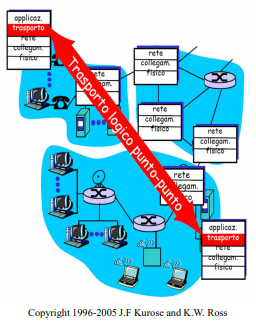
\includegraphics[scale=0.9]{livtrasporto.png}\\\\
\columnbreak


\begin{list}{}{I servizi di trasporto:}
\item Forniscono la \textbf{comunicazione logica} fra processi applicativi di host differenti
\item I \textbf{protocolli} di trasporto vengono \textbf{eseguiti nei sistemi terminali}
\end{list}
\end{multicols}
\subsection{Caratteristiche}
\paragraph{Servizio privo di connessione} In un servizio privo di connessione il \textbf{processo mittente consegna i messaggi al livello di trasporto uno per uno}. Il livello di trasporto \textbf{tratta ogni messaggio come entità singola} senza mantenere alcuna relazione fra essi. I segmenti possono \textbf{non essere consegnati} o \textbf{non arrivare in ordine}.
\paragraph{Servizio orientato alla connessione} In un servizio orientato alla connessione client e server \textbf{stabiliscono una connessione logica}.
\subsection{Servizi offerti}
\paragraph{Multiplexing e Demultiplexing} Il termine \textbf{multiplexing} si riferisce al caso in cui \textbf{un'entità \textit{riceve} informazioni da più di una sorgente}. Lo strato trasporto \textbf{provvede allo smistamento dei pacchetti fra rete e applicazioni}.\\\textbf{Demultiplexing} invece al caso in cui \textbf{un'entità \textit{trasmette} informazioni a più di un destinatario}. Lo strato trasporto provvede all'\textbf{accompagnamento dei flussi dati dai processi verso la rete}, "imbustando" i dati ricevuti dall'alto con un preambolo.\\
Il livello di trasporto effettua il \textbf{multiplexing sul mittente} e il \textbf{demultiplexing sul destinatario}.\\
Si basano sui socket address dei processi e quindi dipendono dal numero di porta su cui i processi sono attivi.
\paragraph{Controllo degli errori}
\section{UDP}
Rispetto al TCP, lo UDP è meno complesso, offre meno servizi, ma è \textbf{più indicato in contesti in cui occorre un controllo completo della temporizzazione} cioè in applicazioni time-sensitive come lo streaming.
\paragraph{Nessuna garanzia} Lo \textbf{User Datagram Protocol} è un \textbf{protocolo di consegna a massimo sforzo}. I segmenti UDP possono andare perduti o essere consegnati fuori sequenza. Notare però che l'affidabilità può essere aggiunta a livello applicazione.
\paragraph{Orientato al messaggio} Ogni \textbf{datagramma UDP è indipendente} dall'altro. I processi devono inviare \textbf{messaggi di dimensioni limitate, incapsulabili in un datagramma UDP}.
\subsection{Proprietà}
\begin{list}{}{}
\item \textbf{Nessuna connessione} quindi non si introduce ritardo.\\\textbf{Semplice}: non viene gestito lo strato di connessione. Le intestazioni sono corte e \textbf{non ha controllo di congestione e di flusso}, quindi si possono sparare dati a raffica.
\item \textbf{Checksum facoltativo}
\item Facile e leggero da gestire, non richiede particolari meccanismi
\item Concepito solo in funzione del DNS e del TFTP, nel 1980
\item Utilizzato spesso in \textbf{applicazioni multimediali}: tolleranza a piccole perdite e sensibilità alla frequenza
\item Altri impieghi: DNS, SNMP\ldots
\end{list}
\pagebreak
\subsection{Datagramma UDP}
\begin{center}
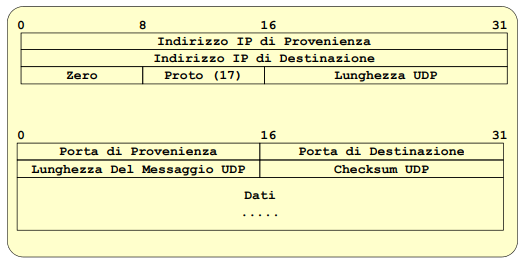
\includegraphics[scale=1]{udpdatagram.png}
\end{center}
\begin{list}{}{}
\item 8 Byte di intestazione
\item La \textbf{prima parte è uno pseudo-header che \textit{non} viene trasmesso}
\item \textbf{Porta}: numeri di porta della comunicazione (per il demultiplexing è usato solo quello di destinazione.\\
La \textbf{porta di provenienza} è un campo facoltativo. Quando è significativo, indica la porta del processo mittente, e può essere considerata come la porta alla quale rispondere in assenza di altre informazioni. Se non è usata, viene riempita col valore 0.
\item \textbf{Lunghezza} del messaggio: lunghezza totale del datagramma UDP, header+dati, è di 65535 Byte.
\item \textbf{Checksum} checksum dell'intero pacchetto, compreso lo pseudo-header ovvero con il controllo dell'indirizzo host). \textbf{Opzionale}, se non è usato è posto a 0xFF (complemento a 1 di 0x00)\\
Controllo dell'errore end-to-end: il pacchetto corrotto è scartato ma l'utente non viene notificato
\item L'indirizzo di livello trasporto è una coppia composta dall'indirizzo IP e dalla porta del destinatario (con indicazione dell'indirizzo IP e della porta del mittente)
\end{list}
\subsection{Calcolo del checksum}
\textbf{Mittente}
\begin{list}{}{}
\item Tratta il contenuto del segmento \textbf{come una sequenza di interi da 16 bit}
\item \textbf{Checksum}: somma (complemento a 1) i contenuti del segmento
\item Il mittente pone il valore della checksum nel campo checksum del segmento UDP
\end{list}
\textbf{Destinatario}
\begin{list}{}{}
\item \textbf{Calcola} il checksum del segmento ricevuto
\item \textbf{Controlla se} il checksum calcolato \textbf{è uguale} al valore del campo checksum
\begin{list}{}{}
\item No -- Errore rilevato
\item Si -- Nessun errore rilevato
\end{list}
\end{list}
\pagebreak
\subsection{TCP vs UDP}
\begin{multicols}{2}
\begin{list}{}{\textbf{UDP}}
\item \textbf{Trasferimento} dati \textbf{non affidabile}
\item \textbf{Non fornisce}: setup della \textbf{connessione}, \textbf{affidabilità}, \textbf{controllo del flusso}, \textbf{controllo della congestione}, \textbf{timing} o \textbf{garanzia di banda}
\item Richiede \textbf{minor overhead}
\end{list}
\columnbreak
\begin{list}{}{\textbf{TCP}}
\item \textbf{Connection-oriented}: richiesto \textbf{handshake} tra client e server
\item \textbf{Trasporto affidabile} tra i processi
\item \textbf{Controllo di flusso}: il mittente non satura il destinatario
\item \textbf{Controllo della congestione}: limita il mittente a rete sovraccarica
\item \textbf{Non fornisce}: \textbf{timing}, \textbf{banda minima}
\end{list}
\end{multicols}
\paragraph{Pro e contro} Nella programmazione di rete si deve ricordare che
\begin{list}{}{}
\item Il TCP offre un \textbf{servizio di trasporto a stream}, quindi si può leggere da un input di rete quanti byte si desiderano
\item L'UDP invece offre un \textbf{servizio a messaggi}, quindi occorre \textbf{leggere tutto} il messaggio in arrivo
\item L'UDP è adeguato per
\begin{list}{}{}
\item Processi che richiedono uno scambio di dati con volume limitato \textbf{in caso di scarso interesse al controllo del flusso e degli errori}
\item Processi con \textbf{meccanismi interni di controllo del flusso e degli errori}
\item Trasmissioni \textbf{multicast}
\item \textbf{Applicazioni interattive in tempo reale} che non tollerano ritardi variabili
\end{list}
\end{list}
\paragraph{Considerazioni} La \texttt{RFC 768} che definisce l'UDP è del 1980, non è stata cambiata o integrata da altre RFC ed è di tre pagine.\\
La \texttt{RFC 793} che definisce il TCP è del 1981, è stata aggiornata o cambiata da diverse altre \texttt{RFC}, ad esempio
\begin{list}{}{}
\item \texttt{2018 - TCP Selective Acknowledgement Options}
\item \texttt{1146 - TCP Alternate Checksum Options}
\item \texttt{2581 - TCP Congestion Control}
\item \texttt{1323 - TCP Extensions for High Performance}
\item \texttt{1693 - An Extension to TCP : Partial Order Service}
\item \texttt{1792 - TCP/IPX Connection Mib Specification}
\end{list}
e la lunghezza totale è di 85 pagine, con un glossario di 67 voci.
\pagebreak
\section{TCP}
% https://elearning.di.unipi.it/pluginfile.php/28129/mod_resource/content/1/L07_Trasporto_TCP_intro.pdf
\subsection{Proprietà}
\paragraph{Orientato allo stream} La \textbf{lunghezza in byte} è \textbf{indefinita} a priori. Il servizio di consegna a destinazione passa esattamente la medesima sequenza di byte che il mittente ha passato al servizio di consegna nell'origine.\\
Il TCP vede i \textbf{dati come un flusso di byte ordinati}, ma \textbf{non strutturati}.\\
\begin{center}
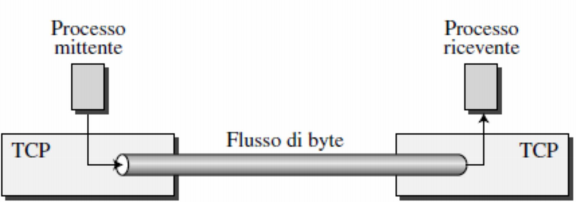
\includegraphics[scale=0.75]{tcpstream.png}
\end{center}
\paragraph{Orientato alla connessione} I processi effettuano un \textbf{handshake} prima dello scambio dei dati. L'\textbf{handshake} è uno \textbf{scambio di informazioni preliminari per preparare il trasferimento dei dati}.\\
Orientato perché \textbf{lo stato della connessione risiede sui punti terminali}, non sugli elementi intermedi della rete (es. router).\\
La \textbf{connessione} è \textbf{vista dagli applicativi} (USERS) \textbf{come un circuito fisico dedicato}. Il \textbf{TCP} è quindi capace di \textbf{fornire servizi di tipo connection-oriented}, mentre il protocollo \textbf{IP} su cui si appoggia è in grado di \textbf{fornire servizi connection-less}.
\paragraph{Connessione full-duplex} Il \textbf{flusso dati tra due host può avvenire contemporaneamente nelle due direzioni}. Le due direzioni sono slegate e la connessione è punto-a-punto.
\paragraph{Trasferimento bufferizzato} Il software del protocollo TCP è libero di \textbf{suddividere lo stream in segmenti indipendenti} (pacchetti), in maniera indipendente dal programma applicativo che li ha generati. Per fare questo è \textbf{necessario} disporre di \textbf{un buffer dove immagazzinare la sequenza di byte}. Appena i dati sono sufficienti per riempire un \textbf{datagramma} ragionevolmente grande, questo viene trasmesso attraverso la rete.
\subsection{Funzioni del segmento TCP}
\begin{list}{}{Funzioni base per il trasferimento di dati:}
\item Capacità di trasferire un \textbf{flusso continuo} di byte
\item Trasferimento bidirezionale (\textbf{full duplex})
\item \textbf{Multiplexing}: consente di assegnare una data \textbf{connessione} ad un dato processo.\\Permette una comunicazione da processo a processo.
\item \textbf{Controllo della connessione}: meccanismi di inizio e fine trasmissione (controllo della sessione)
\item \textbf{Trasferimento dati ordinato e affidabile}: si intende la capacità di correggere tutti i tipi di errore, quali:
	\begin{list}{-}{}
	\item dati corrotti
	\item segmenti persi
	\item segmenti duplicati
	\item segmenti fuori sequenza
	\end{list}
\item \textbf{Controllo di flusso}: evitare di spedire più dati di quanti il ricevitore sia in grado di trattare
\item \textbf{Controllo di congestione}: ha lo scopo di recuperare situazioni di sovraccarico nella rete
\end{list}
\pagebreak
\subsection{Processi e Socket TPC}
\begin{center}
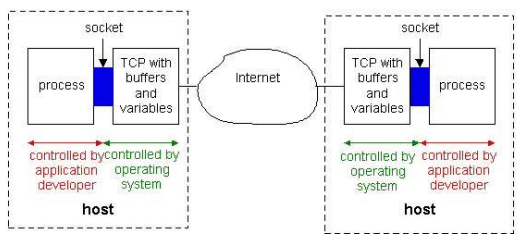
\includegraphics[scale=1]{procsockettcp.png}
\end{center}
I processi in esecuzione su diverse macchine comunicano tra loro mandando messaggi \textbf{attraverso i socket}. Un po' come se ogni processo fosse una casa e ogni socket fosse la porta, \textbf{un socket è la porta tra il processo dell'applicazione e il TCP}.\\
Lo \textbf{sviluppatore ha il controllo su} tutta la parte del \textbf{lato applicazione del socket}, ma \textbf{non può controllare il lato del livello di trasporto}. Al più, lo sviluppatore può specificare alcuni parametri del TCP, come la dimensione massima del buffer e dei segmenti.\footnote{http://www3.gdin.edu.cn/jpkc/dzxnw/jsjkj/chapter2/26.htm}
\subsection{Trasferimento bufferizzato}
\begin{center}
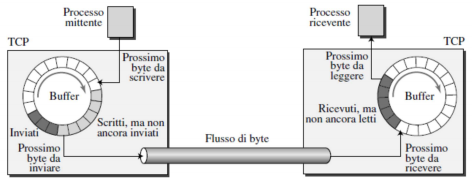
\includegraphics[scale=1]{trasfbufftcp.png}
\end{center}
I \textbf{processi} a livello applicativo \textbf{scrivono e leggono byte nel/dal buffer}, e questo può avvenire a velocità diverse.
\subsection{Segmenti TCP}
\begin{center}
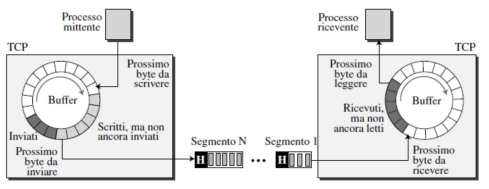
\includegraphics[scale=1]{segmentitcp.png}
\end{center}
Il flusso di byte è \textbf{partizionato in segmenti}: ogni segmento \textbf{ha il suo header} e \textbf{viene consegnato al livello IP}.
\pagebreak
\subsection{Numeri di sequenza e di riscontro}
Il \textbf{TCP numera i byte} anziché i segmenti
\paragraph{Numero di sequenza} Associato al segmento, è il numero (nel flusso) del primo byte (di dati) del segmento. In genere si parte da un \textbf{initial sequence number} generato in modo casuale e diverso da 0.
\paragraph{Numero di riscontro} 1 + numero dell'ultimo byte correttamente ricevuto. I riscontri sono interpretati come \textbf{cumulativi}: se ricevo \texttt{ACK = y} significa che \textit{aspetto il byte} \texttt{y} e quindi ho ricevuto tutti i byte fino a \texttt{y - 1}.
\subsection{Segmento TCP}
\begin{center}
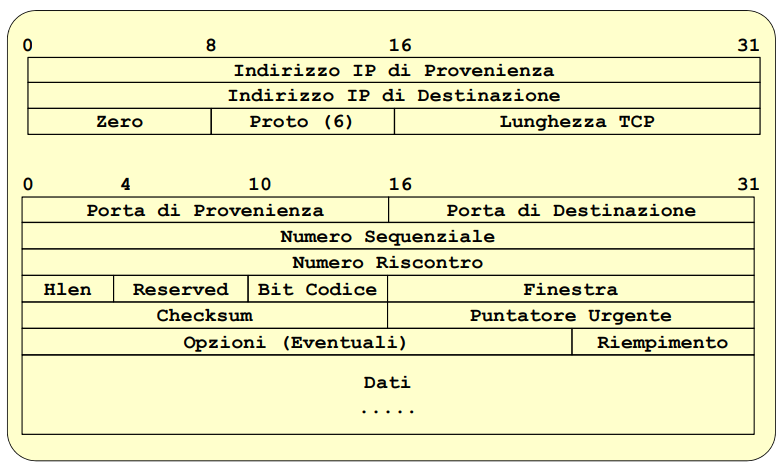
\includegraphics[scale=0.5]{tcpsegment.png}
\end{center}
\begin{list}{}{}
\item Lo \textbf{pseudo header NON viene trasmesso}.\\
Ha valenza logica, contiente \textbf{IP sorgente} e \textbf{destinazione}. Queste info \textbf{vengono inserite} effettivamente \textbf{e trasmesse dal livello inferiore}.\\
\textbf{Proto}: codice del protocollo.\\
\textbf{Lunghezza TCP}: lunghezza del segmento TCP escluso lo pseudoheader, server per il calcolo del checksum.
\item Nel segmento TCP bisogna notare la presenza di:
	\begin{list}{}{}
	\item Numero di \textbf{sequenza}
	\item Numero di \textbf{riscontro}
	\item \textbf{Finestra}
	\end{list}
Essi permettono il \textbf{controllo del flusso}, il meccanismo di \textbf{ritrasmissione} ed il \textbf{riordino} dei pacchetti in ricezione, necessari per la struttura stream-based del TCP
\item Inoltre è presente un campo \textbf{urgent} che permette la trasmissione dei dati "\textbf{fuori banda}", ovvero \textbf{a priorità maggiore degli altri} (la loro gestione però è affidata all'applicazione.
\end{list}
\pagebreak
\subsubsection{Campi del segmento TCP}
\begin{list}{}{}
\item \textbf{Porta} (16 bit): numeri di porta della comunicazione
\item \textbf{Numero di sequenza} (32 bit): è il \textbf{numero di sequenza} nello stream \textbf{del primo byte di dati di questo segmento}.\\Se il flag \texttt{SYN} è settato, allora il numero di sequenza è \texttt{ISN} (Initial Sequence Number) e il primo byte di dati è \texttt{ISN + 1}.
\item \textbf{Numero di riscontro} (32 bit): se il flag \texttt{ACK} è settato, allora questo campo \textbf{contiene il valore del prossimo numero di sequenza che il mittente del segmento si aspetta di ricevere dall'altro host}. Una volta che la connessione è stabilita è sempre inviato.
\item \textbf{Hlen} (4bit): \textbf{lunghezza dell'header} TCP espressa in parole da 4 byte\\La lunghezza dell'header può variare da 20 a 60 byte)
\item \textbf{Bit codice}: sono \textbf{6 flag} e, da sinistra a destra, servono per:
	\begin{center}
	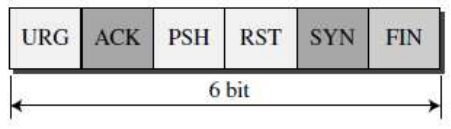
\includegraphics[scale=0.7]{flagtcp.png}
	\end{center}
	\begin{list}{}{}
	\item \texttt{URG}: il campo \textbf{puntatore urgente contiene dati sgnificativi} da trasferire in via prioritaria
	\item \texttt{ACK}: il campo \textbf{numero di riscontro contiene dati significativi}
	\item \texttt{PSH}: \textbf{funzione push}, cioè \textbf{trasferimento immediato} dei dati in un \textbf{segmento dal livello trasporto al livello applicativo}
	\item \texttt{RST}: reset della connessione
	\item \texttt{SYN}: sincronizza il numero di sequenza
	\item \texttt{FIN}: non ci sono altri dati utente -- chiusura della connessione
	\end{list}
\item \textbf{Finestra di ricezione} (16 bit): indica il \textbf{numero di byte di dati} a partire da quello indicato nel campo \textit{numero di riscontro} \textbf{che il mittente di questo segmento è in grado di accettare}.\\Serve per il controllo del flusso.
\item \textbf{Checksum} (16 bit): checksum dell'intero pacchetto (compreso lo pseudo header).\\Serve per il \textbf{rilevamento degli errori} in caso di alterazione dei bit del segmento, e si calcola come per l'UDP (ma \textbf{per il TCP + obbligatorio})
\item \textbf{Opzioni} (facoltativo, lunghezza variabile di massimo 40 byte): \textbf{negoziazione di vari parametri}, ad esempio: dimensione massima del segmento (\texttt{MSS}), selective acknowledgment supportato e blocchi di dati riscontrati selettivamente.\\Le opzioni \textbf{sono sempre multipli di 8 bit} e il loro valore è incluso nel checksum.
\item \textbf{Puntatore urgente} (16 bit): questo campo è un \textbf{offset positivo a partire dal numero di sequenza del segmento corrente}. Viene \textbf{interpretato solo se} il bit \texttt{URG} è uguale a 1.\\\textbf{Punta al primo byte di dati non urgenti} in attesa nella coda di ricezione. Nel segmento contenente dati urgenti \textbf{deve essere presente almeno un byte di dati}.\\
Ad es. se un segmento contiene 400 byte di dati urgenti e 200 byte di dati non urgenti, il puntatore urgente vale 400.
\end{list}
\pagebreak
\subsubsection{Formato del segmento TCP}
\begin{center}
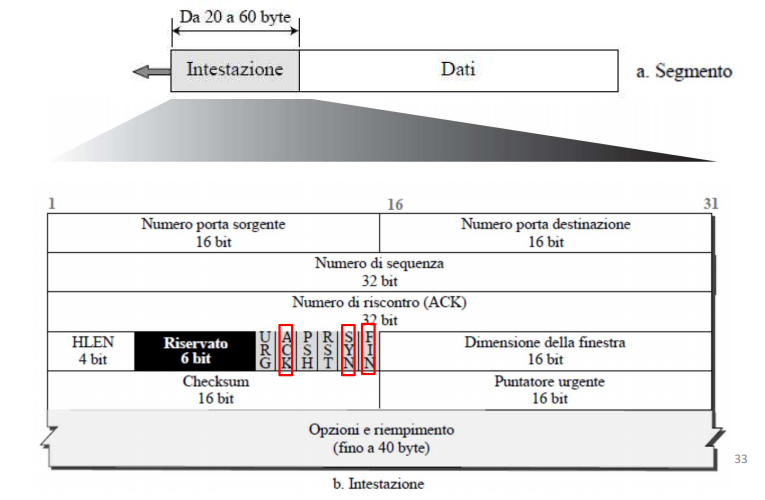
\includegraphics[scale=0.60]{formatosegmentotcp.png}
\end{center}
\subsection{Gestione della connessione}
\subsubsection{Three-Way Handshake}
\paragraph{Handshake a tre vie} Dopo l'handshaking a livello di trasporto, non c'è più distinzione tra client e server. \begin{list}{-}{Sequenza:}
\item Il \textbf{client} \textbf{invia una richiesta di connessione} ad un server TCP.\\
\texttt{SYN} è attivo\\
Il segmento non contiene dati\\
Si trasmette anche un numero di sequenza iniziale casuali\\
Es. \texttt{SYN = 1}, \texttt{clientISN = 41}
\item Il \textbf{server} \textbf{estrae il segmento}, alloca i buffer e le variabili TCP per la connessione.\\
Invia in \textbf{risposta} un \textbf{segmento di connessione garantita} chiamato \texttt{SYNACK}\\
\texttt{SYN} è attivo\\
Il numero di sequenza è il valore iniziale (es. 78)\\
\texttt{ACK} è attivo, il server aspetta \texttt{clientISN + 1} (es. 42)\\
Es. \texttt{SYN = 1}, \texttt{ACK = clientISN + 1}, \texttt{serverISN = 78}
\item Il \textbf{client} \textbf{alloca buffer e variabili} di connessione, poi \textbf{manda un riscontro positivo del messaggio del server}.\\
\texttt{SYN} è inattivo, questo segmento può già trasportare dati.\\
Il prossimo dato datà \texttt{clientISN + 1} (es. 42) ed il client attende \texttt{serverISN + 1} (es. 79)\\
\texttt{SYN = 0}, riscontro \texttt{serverISN + 1}\\
\item \textbf{Inizia lo scambio di dati}
\end{list}
I primi segmenti non hanno carico utile. All'arrivo del primo segmento il server iniziazilizza due buffer e le variabili, necessari per il controllo del flusso e delle congestione.\\
All'arrivo del riscontro del primo segmento il client alloca due buffer e le variabili, per lo stesso motivo.\\
Alla ricezione del terzo segmento la connessione è instaurata.
\pagebreak
\subsubsection{Perché a tre vie}
Esempio degli scalatori:
\begin{center}
\begin{list}{}{}
\item \textit{Ti tengo la corda?} $\rightarrow$ 
\item $\leftarrow$ \textit{Si, tienimi}
\item \textit{Ok} $\rightarrow$
\end{list}
\end{center}
Le cose possono andare male in tanti modi diversi, alcuni di questi sono \textbf{situazioni indistinguibili per A mittente}
\begin{center}
	\begin{multicols}{2}
		\begin{list}{}{}
		\item \textit{Ti tengo la corda?} $\rightarrow$
		\item X $\leftarrow$ \textit{Si, tienimi}
		\item 
		\end{list}
		\begin{list}{}{}
		\item \textit{Ti tengo la corda?} $\rightarrow$ X
		\item
		\item
		\end{list}
	\end{multicols}
\end{center}
Altre invece sono \textbf{situazioni indistinguibili per B destinatario}
\begin{center}
	\begin{multicols}{2}
		\begin{list}{}{}
		\item \textit{Ti tengo la corda?} $\rightarrow$
		\item $\leftarrow$ \textit{Si, tienimi}
		\item \textit{Ok} $\rightarrow$ X
		\end{list}
		\begin{list}{}{}
		\item \textit{Ti tengo la corda?} $\rightarrow$
		\item X $\leftarrow$ \textit{Si, tienimi}
		\item 
		\end{list}
	\end{multicols}
\end{center}
\subsubsection{Esempio}
\begin{center}
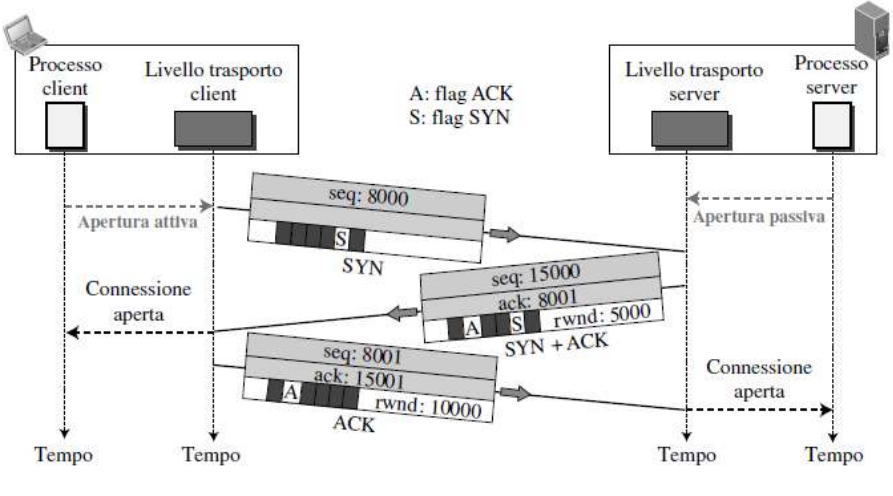
\includegraphics[scale=0.65]{handshakeesempio.png}\\
\texttt{SYN} e \texttt{SYN + ACK} \textbf{non contengono dati} utente ma \textbf{consumano un numero di sequenza}
\end{center}
\pagebreak
\subsubsection{Chiusura della connessione con handshake}
In una connessione TCP normale, dopo l'ACK finale per la chiusura si aspetta un tempo di \textbf{timeout molto grande}.\\
\texttt{timeout = 2 * MSL}\\
\texttt{MSL} è il \texttt{Maximum Segment Lifetime = 120s}
\begin{center}
\includegraphics[scale=0.7]{conntcpclose.png}
\end{center}
Invece con il three-way handshake, \textbf{dopo l'ACK finale la connessione è immediatamente chiusa}.
\begin{center}
\includegraphics[scale=0.7]{conntcphandshakeclose.png}\\
Un \texttt{FIN} che \textbf{non trasporta dati} ma \textbf{consuma un numero di sequenza}. Idem per \texttt{FIN + ACK}.
\end{center}
\pagebreak
\subsection{Half-Close}
\textbf{Uno} dei due processi può \textbf{smettere di inviare dati mentre sta ancora ricevendo dati}.\\
\texttt{TCP.close(conn) = "}\textit{I have no more data to send.}\texttt{"}
\begin{center}
\includegraphics[scale=0.8]{halfclose.png}
\end{center}
Di seguito l'ASF corrispondente agli stati dell'\textbf{half-close}
\begin{center}
\includegraphics[scale=0.7]{halfcloseasf.png}
\end{center}
\subsubsection{Scenario Half-Close}
\begin{center}
\includegraphics[scale=1]{halfclosees.png}
\end{center}
\subsubsection{Stato Time-Wait}
\paragraph{Finale} \textbf{Time-Wait} è lo \textbf{stato finale} in cui \textbf{il capo di una connessione che esegue la chiusura attiva resta prima di passare alla chiusura definitiva} della connessione. Dura \textbf{due volte la Maximum Segment Lifetime}.
\paragraph{MSL} La \textbf{Maximum Segment Lifetime} è la \textbf{stima} del \textbf{massimo periodo di tempo che un pacchetto IP può vivere} sulla rete.\\
Questo tempo è \textbf{limitato} perché \textbf{ogni pacchetto IP può essere ritrasmesso dai router un numero massimo di volte} detto \textbf{hop limit}.\\
Ogni implementazione del TCP sceglie il proprio valore per la MSL (\texttt{RFC 1122} indica 2 minuti, Linux usa 30 secondi).
\paragraph{Perché Time-Wait} Lo stato Time-Wait viene usato dal protocollo \textbf{per due motivi principali}:
\begin{list}{-}{}
\item \textbf{Implementare} in maniera affidabile \textbf{la terminazione della connessione in entrambe le direzioni}.\\
Se l'ultimo \texttt{ACK} della sequenza viene perso, chi esegue la chiusura passiva manderà un ulteriore \texttt{FIN}, chi esegue la chiusura attiva deve mantenere lo stato della connessione per essere in grado di rinviare l'\texttt{ACK}.
\item \textbf{Consentire l'eliminazione di segmenti duplicati} in rete
\end{list}
\pagebreak
\subsection{Stati del TCP}
\begin{center}
\includegraphics[scale=0.7]{tcpstates.png}
\end{center}
\begin{list}{}{Gli stati del TCP:}
\item \textbf{LISTEN}: attesa di una richiesta di connessione remota TCP
\item \textbf{SYN-SENT}: attesa di ricezione di una connection request corrispondente dopo aver mandato la propria connection request
\item \textbf{SYN-RECEIVED}: attesa dell'ACK dopo aver entrambi spedito la connection request
\item \textbf{ESTABLISHED}: connessione aperta, i dati possono essere trasferiti all'utente. Questo è lo stato normale per la fase di trasferimento dati della connessione
\item \textbf{FIN-WAIT-1}: attesa della richiesta di terminazione della connessione dal TCP remoto, oppure un'ACK sulla richiesta di terminazione della connessione precedentemente spedita
\item \textbf{FIN-WAIT-2}: attesa della richiesta di terminazione attiva della connessione dal TCP remoto
\item \textbf{CLOSE-WAIT}: attesa della richiesta di terminazione della connessione dall'utente locale. Si è ricevuta la richiesta di chiusura della connessione e si è già mandato l'ACK, quindi la chiusura passiva è già avvenuta e si attende di avviare la chiusura attiva
\item \textbf{CLOSING}: attesa dell'ACK sulla chiusura della connessione prima di andare in TIME-WAIT
\item \textbf{LAST-ACK}: attesa dell'ACK sulla chiusura attiva della connessione. Chiusura passiva effettuata e chiusura attiva iniziata
\item \textbf{TIME-WAIT}: attesa di abbastanza tempo per assicurarsi che l'host remoto riceva l'ACK per la chiusura della connessione
\item \textbf{CLOSED}: nessuna connessione
\end{list}
\pagebreak
\subsection{Trasferimento Dati Affidabile}
Un \textbf{segmento TCP} può essere \textbf{smarrito} o \textbf{corrotto}. Il TCP crea un \textbf{servizio di trasferimento dati affidabile} sul servizio inaffidabile dell'IP.
\paragraph{Checksum} I \textbf{controlli} sono \textbf{obbligatori} ed i segmenti corrotti vengono scartati.
\paragraph{Riscontri}
\begin{list}{}{}
\item \textbf{Numero di sequenza} di un segmento è il \textbf{numero del primo byte del segmento nel flusso di byte}.\\I numeri di sequenza si applicano ai byte, non ai segmenti trasmessi.
\item \textbf{Numero di riscontro}: \textbf{numero di sequenza successivo} che l'host attende.
\item \textbf{Riscontro cumulativo}: si effettua il \textbf{riscontro dei byte fino al primo byte mancante} del flusso.
\item \textbf{Timer}
\end{list}
\subsubsection{Sequenza e riscontro}
\paragraph{Esempio: Telnet su TCP}
	\begin{list}{}{}
	\item A \texttt{SEQ = 42, ACK = 79, DATA = 'C'} $\longrightarrow$ B\\
	Viene inviato il carattere "C" da A verso B, \textit{ti mando il 42 aspetto il 79}\\
	Nella direzione opposta si rimanda quanto ricevuto
	\item A $\longleftarrow$ \texttt{SEQ = 79, ACK = 43, DATA = 'C'} B\\
	\texttt{ACK} dell'host per ricevuta di "C", restituisco "C", \textit{ti mando il 79, aspetto il 43}
	\item A \texttt{SEQ = 43, ACK = 80} $\longrightarrow$ B\\
	\texttt{ACK} dell'host sulla ricevuta di "C" di ritorno, \textit{ti mando il 43 (o niente) e aspetto l'80}
	\end{list}
\paragraph{Pipeline} Con il \textbf{pipeline} il \textbf{mittente può inviare più segmenti senza attendere il riscontro}. Permette di aumentare la produttività
\begin{list}{}{}
\item A \texttt{SEQ = 42} $\longrightarrow$ B
\item A \texttt{SEQ = 43} $\longrightarrow$ B
\item A $\longleftarrow$ \texttt{ACK = 43} B
\item A $\longleftarrow$ \texttt{ACK = 44} B
\end{list}
\subsubsection{Eventi lato mittente}
\begin{list}{}{}
\item \textbf{TCP riceve i dati dall'applicazione}:
	\begin{list}{-}{}
	\item assegna un numero di sequenza
	\item avvia il timer (intervallo di scadenza -- timeout)
	\end{list}
\item \textbf{Timeout}
	\begin{list}{-}{}
	\item ritrasmette il segmento non riscontrato
	\item riavvia il timer
	\end{list}
\item \textbf{\texttt{ACK} duplicato}\\
Se il mittente \textbf{riceve tre \texttt{ACK} duplicati}, allora significa che il \textbf{segmento successivo a quello riscontrato è andato perso}.\\
\textbf{Ritrasmissione rapida} (fast retransmission) \textbf{prima} dello scadere del timer.
\item \textbf{Ritrasmissione dei segmenti}
	\begin{list}{-}{}
	\item se timeout
	\item se il mittente riceve tre \texttt{ACK} duplicati (fast retransmission)
	\end{list}
\item \textbf{Segmenti fuori sequenza}\\
I dati \textbf{possono arrivare fuori sequenza} ed essere temporaneamente memorizzati dall'entità TCP destinataria. Il TCP \textbf{non dice come} il destinatario \textbf{deve gestire i pacchetti fuori sequenza}, dipende dall'implementazione.\\
Nelle versioni più recenti si implementa \textbf{SACK}: i \textbf{pacchetti fuori sequenza} vengono \textbf{memorizzati}, il \textbf{riscontro} dei pacchetti fuori sequenza e duplicati è \textbf{inviato in \texttt{OPTIONS}}.
\end{list}
\paragraph{Ritrasmissione dovuta a riscontro perso}
\begin{center}
\includegraphics[scale=0.7]{tcplostack.png}
\end{center}
\subsubsection{Eventi lato destinatario}
\textbf{Tutti i segmenti inviati per trasmettere dati includono l'\texttt{ACK}}. Se il destinatario non ha dati da inviare e \textbf{riceve un segmento "in ordine"}, allora \textbf{ritarda l'invio dell'\texttt{ACK} di 500ms} a meno che non riceva un nuovo segmento.\\\\
Se il destinatario \textbf{riceve un segmento atteso ma il precedente non è stato riscontrato} allora \textbf{invia immediatamente l'\texttt{ACK}}.\\\\
Se il destinatario riceve:
\begin{list}{}{}
\item \textbf{segmento fuori sequenza}
\item \textbf{segmento mancante} ("buco" nella sequenza")
\item \textbf{segmento duplicato}
\end{list}
allora \textbf{invia immediatamente l'\texttt{ACK}} indicando il prossimo numero atteso.
\subsubsection{Esempi}
\begin{center}
\textbf{Operatività normale}
\includegraphics[scale=0.65]{tcpnorm.png}\\
\textbf{Segmento smarrito}
\includegraphics[scale=0.68]{tcplostsegm.png}
\pagebreak


\textbf{Ritrasmissione veloce}
\includegraphics[scale=0.7]{tcpfastretr.png}\\
\textbf{Riscontro smarrito}
\includegraphics[scale=0.7]{tcplostack2.png}
\pagebreak


\textbf{Riscontro smarrito corretto da ritrasmissione}
\includegraphics[scale=0.7]{tcpostackretransm.png}
\pagebreak

\textbf{ASM semplificato per il mittente}
\includegraphics[scale=0.6]{tcpasmmit.png}\\
\textbf{ASM semplificato per il destinatario}
\includegraphics[scale=0.6]{tcpasmdest.png}
\end{center}
\pagebreak
\subsection{Calcolo del timeout}
\paragraph{RTO} Il \textbf{Retransmission Timeout}, o tempo di timeout, è \textbf{fondamentale} per il funzionamento del TCP. L'RTO deve essere maggiore dell'RTT (\textbf{Round Trip Time})
\paragraph{RTT} Il Round Trip Time \textbf{tempo trascorso da quando si invia} un segmento \textbf{a quando se ne riceve il riscontro.}. Viene calcolato analizzando gli RTT dei segmenti \textbf{non ritrasmessi}: Sample RTT, stimato per un segmento trasmesso, non per ogni invio)\\
\texttt{EstimatedRTT = (1 - $\alpha$)*EstimatedRTT + $\alpha$*SampleRTT}\\
Poiché SampleRTT può fluttuare, si considera EstimatedRTT, cioè la \textbf{combinazione} dei precedenti valori di EstimatedRTT con il nuovo valore SampleRTT.
\paragraph{} \texttt{RFC 2988} -- Il valore $\alpha$ viene posto a $\frac{1}{8}$, in modo da rendere via via meno importanti gli RTT dei pacchetti più vecchi.
\begin{center}
\texttt{EstimatedRTT = 0.875*EstimatedRTT + 0.125*SampleRTT}
\end{center}
\paragraph{Variabilità} Oltre al valore RTT stimato, è necessaria anche una \textbf{stima della variabilità} di RTT, data dalla seguente formula che \textbf{stima di quanto SampleRTT si discosta da EstimatedRTT}:
\begin{center}
\texttt{RTT$_{DEV}$ = (1 - $\beta$)RTT$_{DEV}$ + $\beta$*|RTT$_{SAMPLE}$ - RTT$_{ESTIMATED}$|}
\end{center}
\paragraph{} \texttt{RFC2988} -- Il valore di $\beta$ viene posto a $\frac{1}{4}$
\paragraph{Calcolo del timeout} Una volta ottenuti questi valori, il timeout viene normalmente calcolato come:
\begin{center}
\texttt{RTO = RTT$_{ESTIMATED}$ + 4*RTT$_{DEV}$}
\end{center}
Inoltre in molte implementazioni, dopo un errore (es. \texttt{ACK} non ricevuto) \textbf{si raddoppia il timeout}. Questo è un primo meccanismo di controllo della congestione.
\subsection{Finestra di trasmissione}
\paragraph{Sliding Window} Il \textbf{controllo del flusso} (flow control) del TCP si basa sulla \textbf{finestra di trasmissione}. La finestra è \textbf{sovrapposta alla sequenza da trasmettere}, viene \textbf{negoziata dinamicamente} e viene \textbf{fatta avanzare alla ricezione di un \texttt{ACK}}.\\
\begin{center}
\includegraphics[scale=0.7]{tcpwindow.png}
\end{center}
\pagebreak
\begin{center}
\textbf{Mittente}\\
\includegraphics[scale=0.7]{tcpwindow2.png}\\
\textbf{Destinatario}\\
\includegraphics[scale=0.7]{tcpwindow3.png}
\end{center}
\textbf{Ogni host} imposta buffer di invio e ricezione. Il \textbf{processo destinatario legge} i dati dal buffer di ricezione (\textbf{non necessariamente nell'istante in cui arrivano})\\
Con \textbf{controllo di flusso} si intende \textbf{la capacità del mittente di evitare la possibilità di saturare il buffer del ricevitore}, modulando la propria frequenza di invio. Quindi si \textbf{mette in relazione la frequenza di invio} del mittente \textbf{con al frequenza di lettura} dell'applicazione ricevente.
\paragraph{Receive Window} Il TCP implementa questa funzionalità con una \textbf{variabile} detta \textbf{receive window}, \textbf{mantenuta dal mittente}. Questa variabile \textbf{fornisce un'idea di quanto spazio è ancora a disposizione} nel buffer del ricevitore. Tale valore è comunicato nel \textbf{campo window} dell'header TCP.
\begin{center}
\includegraphics[scale=0.7]{tcprecwindow.png}
\end{center}
Lo spazio disponibile nel buffer del destinatario è:\\
\texttt{RcvWindow = RcvBuffer - (LastByteReceived - LastByteRead)}\\\\
\textbf{RcvWindow} è \textbf{dinamica}, il \textbf{destinatario comunica la dimensione} di RcvWindow al mittente. Il mittente si assicura che:\\
\texttt{LastByteSent - LastByteAcked $<$ RcvWindow}\\
Se RcvWindow = 0, il mittente mandera \textbf{segmenti "sonda"} di 1 byte per ricevere l'aggiornamento sulla dimensione di RcvWindow. Di seguito un esempio:
\begin{center}
\includegraphics[scale=0.7]{tcprcvwinesempio.png}
\end{center}
\subsection{Controllo della congestione}
\texttt{RFC 2581}
\paragraph{Origine} Il fenomeno della congestione ha origine quando una o più delle sorgenti \textbf{tentano di richiedere più banda di quella disponibile sul percorso}. Troppe sorgenti che trasmettono troppi dati ad una velocità troppo alta, per cui \textbf{la rete non può gestirli}.\\
Il \textbf{traffico eccessivo può provocare}:
\begin{list}{}{}
\item \textbf{lunghi ritardi}, accodamenti nei buffer dei router
\item \textbf{perdita di pacchetti}, overflow nei buffer dei router
\end{list}
\paragraph{Controlli} Il protocollo TCP prevede il \textbf{controllo della congestione}, \textbf{imponendo} a ciascun mittente di \textbf{limitare la frequenza di invio di pacchetti sulla connessione}, in funzione della \textbf{congestione percepita}.\\
\textbf{Capacità del TCP di adattarsi alla velocità di rete}: se il TCP percepisce scarso traffico, aumenta la frequenza di invio, altrimenti la diminuisce.\\
\textbf{Controllo di congestione punto-punto}: nessun supporto esplicito della rete, la \textbf{congestione} è \textbf{dedotta dai sistemi terminali}
\pagebreak
\begin{multicols}{2}
\textbf{Come gestire entrambi i tipi di congestione}?
\begin{list}{}{}
\item \textbf{Receiver window}: dipende dalla dimensione del buffer di ricezione
\item \textbf{Congestion window}: basata su una stima della capacità di rete
\end{list}
I byte trasmessi corrispondono alla \textbf{dimensione della finestra più piccola}:\\
\texttt{dimFinestraInvio = min(rWnd, cWnd)}

\columnbreak
\includegraphics[scale=0.6]{congestionetipi.png}
\end{multicols}
\subsubsection{Algoritmo per il controllo della congestione}
\paragraph{Algoritmo} L'algoritmo che il \textbf{mittente TCP} utilizza per \textbf{regolare la propria frequenza di invio} in funzione della congestione rilevata, è costituito da \textbf{tre passi}:
\begin{enumerate}
\item \textbf{Partenza}, \textit{slow start}
\item \textbf{AIMD}: \textbf{incremento additivo} e \textbf{decremento moltiplicativo}
\item \textbf{Ripresa veloce}, \textit{fast recovery}
\item \textbf{Reazione ai time-out}
\end{enumerate}
cWnd impone un \textbf{vincolo} alla frequenza di immissione del traffico sulla rete, in base alla congestione percepita.
\subsubsection{cWnd}
Solitamente è misurata in termini di \textbf{Maximum Segment Size}, MSS.\\
1 MSS è la \textbf{quantita massima di dati trasportabili da un segmento}.
\begin{list}{}{}
\item Viene \textbf{determinato in base alla MTU} (Maximum Transfer Unit), cioè alla lunghezza massima del payload del frame di collegamento inviabile dall'host mittente
\item MSS scelto in modo tale che \textbf{il segmento TCP, incapsulato dentro il pacchetto IP, stia dentro un singolo frame} di collegamento.
\end{list}
RTT (\textbf{Round Trip Time}) è il \textbf{tempo impiegato da un segmento per effettuare il percorso di andata e ritorno}.
\subsubsection{AIMD}
\textbf{Additive Increase Multiplicative Decrease}\\\\
Il TCP del mittente \textbf{aumenta proporzionalmente la propria finestra di congestione ad ogni ACK ricevuto}. Di quanto aumenta?\\
Ad ogni ACK la cWnd viene incrementata in modo che si abbia una \textbf{crescita pari ad 1 MSS per ogni RTT} (\textbf{congestion avoidance})\\
Incremento di \texttt{1MSS * (MSS/cWnd)}\\
Ad esempio se \texttt{cWnd = 4MSS} allora l'incremento è di \texttt{MSS/4}\\\\
Il TCP del mittente \textbf{dimezza la propria finestra di congestione ad ogni evento di perdita}, ad es. timeout o ACK duplicati.\\


\pagebreak
\textbf{Andamento della dimensione della cWnd nel tempo}: andamento a "sawtooth"
\begin{center}
\includegraphics[scale=0.65]{cwndgraph.png}
\end{center}
\subsubsection{Slow Start}
All'inizio, la finestra di congestione cWnd è posta pari a 1 MSS: equivale a dire che la \textbf{frequenza di invio è pari a 1 MSS/RTT}.
\subparagraph{Esempio} Se MSS = 500Byte e RTT = 200ms si ha una frequenza di invio di circa 20 Kb/s. Se ho una banda da 1 Mb/s impiegherò molto tempo per sfruttarla con un incremento lineare.\\\\
cWnd viene incrementata di 1 MSS ad ogni \texttt{ACK}. L'effetto è che cWnd \textbf{raddoppia ad ogni \texttt{RTT}} avendo così una \textbf{crescita esponenziale} fino ad un errore, poi cWnd dimezza.
\begin{center}
\includegraphics[scale=0.7]{slowstartgraph.png}
\end{center}
\pagebreak
\subsubsection{Politica Reno per il controllo della congestione}
\paragraph{Soglia} Viene definita una \textbf{variabile "soglia"}, alla quale è assegnato un valore alto (ad esempio 64 Kb).\\
Questa soglia \textbf{determina quando termina la slow start ed inizia la congestion avoidance (AIMD)}.
\begin{list}{}{}
\item \textbf{cWnd $<$ soglia}: cWnd \textbf{aumenta esponenzialmente} (\textit{slow start})
\item \textbf{cWnd $>$ soglia}: cWnd \textbf{aumenta linearmente} (\textit{AI})
\end{list}
\paragraph{Evento di perdita} Se ho \textbf{3 \texttt{ACK} duplicati} pongo prima la \textbf{soglia a metà di cWnd} e poi \textbf{cWnd = soglia + 3 MSS} (\textit{fast recovery})\\
Se ho \textbf{un \texttt{ACK} perso per timeout} pongo la \textbf{soglia a metà di cWnd} e pongo \textbf{cWnd = 1 MSS} (\textit{slow start})
\paragraph{Nella fast recovery} Se avviene un \textbf{timeout} si va in \textbf{slow start}, se arriva un \texttt{ACK} \textbf{non duplicato} si va in \textbf{congestion avoidance}.
\paragraph{Esempio di controllo della congestione con TCP Reno}
\begin{center}
\includegraphics[scale=0.75]{congestionerenoesempio.png}
\pagebreak

\textbf{TCP Reno}\\
\includegraphics[scale=0.65]{tcpreno.png}
\end{center}
\subsubsection{Politica Tahoe per il controllo della congestione}
Versione precedente della politica Reno: \textbf{timeout e 3 \texttt{ACK} duplicati sono trattati allo stesso modo}.
\begin{center}
\includegraphics[scale=0.75]{tcptahoeesempio.png}\\
\includegraphics[scale=0.65]{tcptahoe.png}
\end{center}
\subsection{Throughput}
Indicando con \texttt{W} il \textbf{valore massimo di byte della finestra} (ovvero quando si verifica l'errore), il \textbf{TCP in regime stazionario} offre il seguente throughput medio:
\begin{center}
\texttt{throughput = $\frac{0.75 * W}{RTT}$}
\end{center}
Calcolo macroscopico che ignora le fasi di slow start.
\begin{list}{}{Con \texttt{W} la dimensione della finestra alla perdita:}
\item Quando la finestra è \texttt{W}, il troughput è $\frac{W}{RTT}$
\item Appena dopo la perdita, la finestra è ridotta a $\frac{W}{2}$ e il throughput a $\frac{W}{2 * RTT}$
\item Throughput medio: \texttt{0.75 * RTT}
\end{list}
\subsection{Fairness}
\paragraph{Ipotesi} \begin{list}{}{}
\item \textbf{K connessioni TCP} esistono su un \textbf{unico link di capacità R bit/s}
\item \textbf{Non ci sono altri protocolli} esistenti sullo stesso link
\end{list}
\paragraph{Risultato} Ognuna delle \textbf{connessioni TCP} tende a \textbf{trasmettere a R/K bit/s}.
\subsection{Transmission Control Block}
\paragraph{Struttura dati} Poiché ogni connessione è distinta, bisogna \textbf{mantenere delle informazioni} su ogni connessione \textbf{separatamente}.
\paragraph{TCB} Il TCP usa una struttura dati speciale per questo scopo, chiamata \textbf{Transmission Control Block} o TCB.\\
Il TCB contiene tutte le informazioni a proposito della connessione, come \textbf{i due numeri di socket} che la identificano e \textbf{i puntatori ai buffer} dove vengono mantenute le informazioni in arrivo e in partenza.\\
Il TCB è anche usato per \textbf{implementare il meccanismo delle sliding windows}. Mantiene delle variabili che tengono traccia dei \textbf{numeri di byte ricevuti e riscontrati}, \textbf{byte ricevuti e non riscontrati}, \textbf{dimensione attuale della finestra} e così via.\\
Ovviamente, \textbf{ogni dispositivo mantiene il proprio TCB per la connessione}.
\pagebreak
\section{Livello di Rete}
Il \textbf{livello di rete} si occupa di \textbf{realizzare una connessione logica fra host diversi}: interconnessione di reti eterogenee.\\
\textbf{Internet} è una \textbf{rete logica} costituita da un \textbf{insieme di reti fisiche}. Il livello di rete offre un'astrazione che consente ad host e reti eterogenee di funzionare dal punto di vista logico come una singola rete.\\\\
\textbf{Offre servizi} al livello di trasporto.\\
\textbf{Utilizza servizi} del livello datalink.
\subsection{Servizi}
\begin{list}{}{}
\item Suddivisione in \textbf{pacchetti}
\item \textbf{Routing} (instradamento)
\item \textbf{Forwarding} (inoltro)
\end{list}
\subsection{Architettura di rete IP}
\begin{multicols}{2}
\includegraphics[scale=0.65]{livelloretearch.png}
\columnbreak

Dal mittente, il livello di rete \textbf{riceve i segmenti dal livello di trasporto} e \textbf{li incapsula nei datagrammi}.\\\\
Dal destinatario, \textbf{consegna i segmenti al livello di trasporto} (demux TCP o UDP)\\\\
I protocolli del livello di rete sono in ogni host e router. Il router esamina i campi intestazione in tutti i datagrammi IP che lo attraversano, e li inoltra da un collegamento in entrata ad uno in uscita.
\end{multicols}
\pagebreak
\subsection{Protocol Data Units}
\begin{center}
\includegraphics[scale=0.715]{livelloretepdu.png}
\end{center}
\subsection{Alcuni protocolli della Suite TCP/IP}
\begin{center}
\includegraphics[scale=0.75]{livelloreteprotocols.png}
\end{center}
\pagebreak
\section{IP}
\paragraph{Internet Protocol} \texttt{RFC 791}
\begin{list}{}{Caratteristiche:}
\item \textbf{Connection less}: non c'è circuito virtuale né fisico fra i due host a livello IP, non c'è garanzia di sequenzialità.
\item \textbf{Non affidabile}: non prevede meccanismi di controllo dell'errore. "\textit{Send and pray}".
\item \textbf{Best effort}: non prevede garanzie sulla QoS (\textbf{Quality of Service}), sul \textbf{tempo di consegna} dei datagrammi e sul \textbf{controllo di flusso}.\\
I modelli di QoS vengono implementati dai router (es: DiffServ)
\end{list}
\subsection{Funzioni}
\subsubsection{Inoltro}
\paragraph{Forwarding} Trasferimento del pacchetto sull'appropriato collegamento d'uscita
\begin{center}
\includegraphics[scale=0.7]{ipforwarding.png}
\end{center}
\subsubsection{Instradamento}
\paragraph{Routing} Processo decisionale di scelta del percorso verso una destinazione (\textbf{algoritmi di routing} o algoritmi di instradamento)
\subsubsection{Indirizzamento}
Strumento per identificare gli host nella rete interconnessa
\paragraph{Modello datagram} Il modello datagram (senza connessione) per la consegna dei dati:
\begin{list}{}{}
\item Segmentazione e riunificazione dei pacchetti (adattamento al data link)
\item \textbf{Controllo degli errori} solo dell'header
\item \textbf{Verifica TTL}
\end{list}
\pagebreak
\subsection{Multiplexing / Demultiplexing}
\begin{center}
\includegraphics[scale=0.7]{ipmuxdemux.png}
\end{center}
\subsection{Datagramma IP}
\subsubsection{Formato}
\begin{center}
\includegraphics[scale=1]{ipdatagramscheme.png}\\
\includegraphics[scale=0.7]{ipdatagramformat.png}
\end{center}
\pagebreak
\subsubsection{Campi}
\begin{list}{}{}
\item \textbf{Versione}, 4 bit: specifica la versione usata. Attualmente IPv4 o IPv6.
\item \textbf{Hlen}, 4 bit: lunghezza dell'header espressa in parole da 32 bit. Tipicamente vale 0101, cioè 20 Byte.
\item \textbf{Tipo di servizio}, 8 bit: serve per "colorare" il datagramma IP (basso ritardo, affidabilità\ldots). Nella \texttt{RFC 791} c'è una prima classificazione, ma si veda anche \texttt{RFC2474}.
\item \textbf{Lunghezza del datagramma}, 16 bit: lunghezza di tutto il datagramma in byte, header incluso. Max 65535 Byte (nella pratica, max 1500 Byte).
\item \textbf{Identificazione}, \textbf{flag}, \textbf{offset}: campi per la frammentazione
\item \textbf{Tempo di vita}, 8 bit: ad ogni passaggio da un router viene decrementato, quando raggiunge lo 0 viene scartato. Assicura che \textbf{eventuali circuiti ad anello non provochino traffico perpetuo sulla rete}.\\
Il valore dipende dal S.O., esempi: 30, 64, 128, 255.
\item \textbf{Protocollo}, 8 bit: in ricezione indica quale protocollo dello strato superiore deve ricevere i dati. Inizialmente la tabella era nella \texttt{RFC 1700}, attualmente è un database online su \texttt{iana.org}.
\item \textbf{Checksum dell'intestazione}, 16 bit: ad ogni router (TTL cambia ad ogni hop) viene calcolato il checksum \textbf{della sola intestazione} ponendo questo campo pari a 0. Se si ottiene un errore si scarta il datagramma.
\item \textbf{Indirizzi sorgente e destinazione}, 32 bit: indirizzi IP mittente e destinatario
\item \textbf{Opzioni}, variabile multiplo di 32 bit: principalmente usati a scopo di test o debug
\item \textbf{Dati}: i dati effettivamente trasportati
\end{list}
\subsection{Frammentazione}
La \textbf{MTU} pone un \textbf{limite alla lunghezza dei datagrammi IP} e tratte diverse possono porre limiti diversi.\\
\textbf{Maximum Transfer Unit} è la quantità massima di dati trasportata dal protocollo di collegamento (\textbf{in un frame}). Può variare da una tecnologia di collegamento all'altra.
\begin{center}
\includegraphics[scale=0.7]{ipmtu.png}
\end{center}
\paragraph{Meccanismo di frammentazione} Se un router \textbf{riceve un datagramma la cui dimensione supera l'MTU della rete su cui deve spedirlo, lo spezza} in due o più datagrammi più piccoli detti \textbf{frammenti}.\\
Il riassemblaggio è effettuato dall'entità rete nel sistema destinatario. \textbf{Se qualche frammento non arriva a destinazione si butta via tutto il datagramma}.\\\\
\textbf{Ciascun frammento è un datagramma IP indipendente e completo}, che viene trasmesso attraverso una serie di reti fisiche indipendentemente dagli altri.
\pagebreak
\paragraph{Ricomporre i frammenti} Per ricomporre si usano i flag \textbf{identificazione}, \textbf{flag} e \textbf{offset}.
\begin{list}{}{}
\item \textbf{Identificazione}, 16 bit: identificatore associato al datagramma dall'host sorgente. Associato a IP sorgente e destinazione \textbf{identifica quel datagramma in un intervallo di tempo ragionevolmente lungo}. I \textbf{frammenti mantengono il valore di questo campo} e il destinatario riconosce i frammenti che vanno assemblati insieme.
\item \textbf{Offset}, 13 bit: indica la posizione relativa come multiplo di 8 Byte. Serve ad ordinare i frammenti nell'assemblaggio.\\
I frammenti \textbf{devono essere multipli di 8 Byte}, ed il primo frammento ha offset = 0.
\item \textbf{Flag}, 3 bit: serve ad identificare l'ultimo frammento.
\begin{list}{}{3 bit}
\item Il bit 0 è \textbf{riservato}, per ora vale sempre 0
\item Il bit 1 è \textbf{do not fragment}. Vale
\begin{list}{}{}
\item 0, se il pacchetto \textbf{può} essere frammentato
\item 1, se il pacchetto \textbf{non può} essere (ulteriormente) frammentato
\end{list}
\item Il bit 2 è \textbf{more fragments}. Vale
\begin{list}{}{}
\item 0, se il pacchetto \textbf{è l'ultimo} frammento
\item 1, se il pacchetto \textbf{non è l'ultimo} frammento
\end{list}
\end{list}
\end{list}
\paragraph{Ripetuto} Il processo di frammentazione \textbf{può essere ripetuto}, ad es. nel caso in cui un frammento viene inoltrato su un collegamento con MTU ancora più piccolo.
\paragraph{Critico} La ricostruzione del datagramma è un \textbf{processo critico}, richiede risorse e se un frammento manca il datagramma è scartato.
\begin{center}
\includegraphics[scale=0.8]{ipframmentazioneesempio.png}
\end{center}
\pagebreak
\section{Indirizzamento IP}
Ogni host è connesso ad internet attraverso un'\textbf{interfaccia di rete}, confine fra host e il collegamento su cui vengono inviati di datagrammi. Ad \textbf{ogni interfaccia} è \textbf{assegnato un indirizzo IP}.\\
I \textbf{router devono necessariamente essere connessi ad almeno due collegamenti}.
\subsection{Indirizzi IPv4}
Gli indirizzi IP sono costituiti da \textbf{32 bit}, cioè 4 Byte, rappresentati in \textbf{notazione decimale puntata}.\\
Es \texttt{10000000  00001011  00000011  00011111} $\longrightarrow$ \texttt{128.11.3.31}
\paragraph{Divisione} Ogni host ha un \textbf{indirizzo univoco sulla rete}, diviso in due parti, \textbf{network ID} e \textbf{host ID}, che identificano una rete IP su internet e l'host in quella rete IP.
\begin{center}
\includegraphics[scale=0.6]{ipnethostid.png}
\end{center}
\subsection{Classful addressing}
\begin{center}
\includegraphics[scale=0.65]{ipclassfuladdresing.png}
\end{center}
\begin{list}{Classe}{5 \textbf{classi di indirizzi} IP:}
\item \textbf{A}: (0.0.0.0 $\rightarrow$ 127.255.255.255) 7 bit per 128 reti, 24 bit per 16M di host 
\item \textbf{B}: (128.0.0.0 $\rightarrow$ 191.255.255.255) 14 bit per 16k reti, 16 bit per 64k host
\item \textbf{C}: (192.0.0.0 $\rightarrow$ 223.255.255.255) 21 bit per reti e 8 bit per 256 host 
\item \textbf{D}: (224.0.0.0 $\rightarrow$ 239.255.255.255) riservata a \textbf{multicasting} 
\item \textbf{E}: (240.0.0.0 $\rightarrow$ 255.255.255.255) riservata per \textbf{usi futuri} 
\end{list}
\subsection{Strategie di addressing}
Il \textbf{classful addressing è poco flessibile}, si può optare quindi per un \textbf{classless addressing}.\\
Inoltre, gli \textbf{indirizzi IP si stanno progressivamente esaurendo}. La specifica IPv6 ha indirizzi di 128 bit invece che di 32 bit, e potrebbe risolvere questo problema.
\pagebreak
\paragraph{Esempi di indirizzi IP}
\begin{list}{}{}
\item 15.10.10.90: classe A (primo numero tra 0 e 127), quindi 10.10.90 indica l'host
\item 130.250.42.53: classe B (primo numero tra 128 e 191), quindi 42.53 indica l'host
\item 196.234.12.14: classe C (primo numero tra 192 e 223), quindi 14 indica l'host
\end{list}
%https://elearning.di.unipi.it/pluginfile.php/28806/mod_resource/content/1/L10_Rete_IntroIP.pdf
\pagebreak
\section{Esercizi}
\subsection{SMTP}
\paragraph{Testo} L’utente mickey@disney.com invia dal suo PC una email a donald@disney.com.\\
Indicare la sequenza di comandi SMTP inviati e ricevuti dal PC di mickey@disney.com se:
\begin{enumerate}
\item Il mailserver disney.com non è raggiungibile
\item Il mailserver disney.com è raggiungibile
\end{enumerate}
\paragraph{Soluzione}
\begin{enumerate}
\item Il PC del mittente non può stabilire una connessione TCP con il mailserver, di conseguenza nessun messaggio SMTP può essere inviato o ricevuto
\item Il mittente stabilisce una connessione TCP con il mailserver, e avviene lo scambio dei seguenti comandi:
\begin{verbatim}
R: 220 service ready
I: HELO . . .
R: 250 OK
I: MAIL FROM: mickey@disney.com
R: 250 OK
I: RCPT TO: donald@disney.com
R: 250 OK
I: DATA
I: . . .
I: . . .
I: .
R: 250 OK
I: QUIT
R: 221 service closed
\end{verbatim}
Notare che il corpo del messaggio termina sempre con \texttt{<CRLF>.<CRLF>}.
\end{enumerate}
\pagebreak
\subsection{DNS}
\paragraph{Testo} Un host deve risolvere il nome simbolico \texttt{host.engineering.vanderbilt.edu}, il cui indirizzo IP non è noto al suo resolver (i.e. servizio DNS dell’host).\\
Supponendo che la gerarchia dei name server abbia 4 livelli, indicare – giustificando la risposta - il numero di messaggi DNS che, nel caso peggiore, circoleranno in Internet per risolvere tale nome
simbolico, se:
\begin{enumerate}
\item Si utilizza ad ogni livello una risoluzione ricorsiva
\item Si utilizza ad ogni livello una risoluzione iterativa
\end{enumerate}
\paragraph{Soluzione}
\begin{multicols}{2}
\begin{enumerate}
\item Bisogna percorrere tutto l'albero dei nameserver, dal locale fino ad un root server, e poi da questo all'authoritative name server che, nel caso peggiore, è il nameserver locale di \texttt{engineering.vanderbilt.edu}, per poi tornare indietro.\\
In totale sono 4 + 4 messaggi + 2 dal resolver al nameserver locale del client e viceversa.\begin{center}
\includegraphics[scale=0.3]{dnsqueryricorsiva.png}
\end{center}
\item Analogamente i messaggi saranno sempre 10, perché i nameserver coinvolti sono 4, nel caso pessimo, più i 2 messaggi tra il nameserver locale del client e il resolver.
\begin{center}
\includegraphics[scale=0.3]{dnsqueryiterativa.png}
\end{center}
\end{enumerate}
\end{multicols}
\pagebreak
\subsection{TCP}
\paragraph{Testo} Un client C chiede la pagina web \texttt{http://www.acme.com/home/products.html} al server B di \texttt{www.acme.com} con una GET che è contenuta in un segmento TCP il cui payload (campo Dati) è lungo X byte. Indicare, giustificando la risposta, i valori dei campi sequence number, \texttt{ACK} number, e dei flags \texttt{ACK} e \texttt{SYN} e lunghezza del campo DATA, in ciascuno dei segmenti che C e B si scambiano per aprire la connessione nell’ipotesi che l’\texttt{ACK} finale dell’apertura della connessione sia inviato in piggybacking assieme alla GET. Si supponga che in B ed in C rWnd sia molto grande, che non scada alcun timeout, che non ci siano errori di trasmissione, che nessun segmento vada perduto, e che il numero di sequenza iniziale di C sia 1111 e quello di B sia 2222
\paragraph{Soluzione}
\begin{center}
\includegraphics[scale=1]{es_tcp1.png}
\end{center}
\subparagraph{Piggybacking} L'invio dei primi dati e l'invio dell'ultimo \texttt{ACK} dell'handshake sono uniti.
\paragraph{Testo} Un client C ha stabilito una connessione TCP con un server web S per scaricare una pagina web che consiste di tre oggetti. Al tempo t, subito dopo avere inviato la richiesta per il terzo oggetto, l’host di C invia a S un segmento con il flag FIN a true.\\
Indicare, giustificando la risposta, il tempo minimo necessario al TCP di C per chiudere definitivamente la connessione supponendo che:
\begin{enumerate}
\item La dimensione del terzo oggetto sia 1.5 MSS
\item RTT sia costantemente 700ms e che il Maximum Segment Lifetime sia 1100ms
\item Tutti i segmenti vengano ricevuti corretti ed in ordine, e che il valore di cwnd del TCP di S sia 1MSS quando esso riceve il FIN inviato dall’host di C. Trascurare i tempi di preparazione e di trasmissione dei segmenti e assumere che S abbia già a disposizione tutti i dati da inviare.
\end{enumerate}
\paragraph{Soluzione} \texttt{3RTT + 2MSL = 4300ms}\\
Il TCP di C riceve al tempo t + RTT il riscontro S1 del segmento FIN da lui inviato. Se S1 trasporta in piggybacking il primo MSS dei dati del terzo oggetto e il TCP di C invierà un riscontro C2 per tali dati, quindi S potrà inviare l’ultima porzione di dati e attenderne il riscontro, infine il TCP di S invierà un segmento con il flag FIN a true. Il TCP di C invierà un riscontro del FIN e considererà chiusa la connessione dopo avere atteso 2MSL, ovvero al tempo t + 3RTT + 2MSL = t + 4300 msec.
\pagebreak
\paragraph{Testo} Si descriva il meccanismo di controllo di flusso del TCP
\paragraph{Soluzione possibile}  Si intende con controllo di flusso la capacità del mittente di evitare la possibilità di saturare il buffer del ricevitore. Infatti, a livello TCP ogni host imposta un buffer di invio e uno di ricezione. Il processo applicativo destinatario legge i dati dal buffer di ricezione (non necessariamente nell’istante in cui arrivano). Il controllo di flusso ha lo scopo di regolare la frequenza di invio del mittente in base alla frequenza di lettura dell’applicazione ricevente allo scopo di non saturare il buffer del ricevente. TCP implementa questa funzione tramite una variabile detta receive window mantenuta nel mittente: questa variabile fornisce un’idea di quanto spazio è ancora a disposizione nel buffer del ricevitore. Tale valore è comunicato nel campo window dell’header TCP dall’host destinatario.
\begin{list}{}{}
\item Il valore di receive window RcvWindow= RcvBuffer-( LastByteReceivedLastByteRead).
\item L’host destinatario comunica la dimensione di RcvWindow al mittente.
\item Il mittente si assicura che LastByteSent-LastByteAcked $<$ RcvWindow pari ovvero alla quantità di dati trasmessi e non ancora riscontrati.
\end{list}
Nelle situazioni in cui il buffer risulta pieno (RcvWindow=0), il mittente continua a mandare segmenti sonda di 1 byte per ricevere l’aggiornamento sulla dimensione di RcvWindow.
\paragraph{Testo}  Due host H1 e H2 comunicano tramite un canale che attraversa tre router R1, R2 e R3 e 4 link di capacit`a C1, C2, C3 e C4, rispettivamente come mostrato in figura. La comunicazione avviene tramite commutazione di pacchetto con trasmissione di tipo store and forward.\\
Assumendo che il ritardo di propagazione sia trascurabile, che i ritardi di accodamento nei router R1, R2 e R3 sia rispettivamente a1, a2 e a3, e che il ritardo di elaborazione nei tre router sia uguale a 1 ms, dire quanto tempo `e necessario per la trasmissione da H1 a H2 di un pacchetto di dimensione L nel seguente caso:
\begin{list}{-}{}
\item L = 10 KBytes
\item C1 = C2 = C3 = C4 = 2 Mbps
\item a1 = a3 = a4 = 0.01 s
\end{list}
\begin{center}
\includegraphics[scale=1]{es_tcp6testo.png}
\end{center}
\paragraph{Soluzione} Il ritardo introdotto da ogni router `e dato dalla somma
tra: ritardo di trasmissione, ritardo di propagazione, ritardo di
accodamento e tempo di elaborazione. In particolare:
\begin{list}{-}{}
\item il tempo di trasmissione di H1 è pari a L/C1 = 40 ms.
\item il tempo di trasmissione di R1 è pari a L/C2 = 40 ms.
\item il tempo di trasmissione di R2 è pari a L/C3 = 40 ms
\item il tempo di trasmissione di R3 è pari a L/C4 = 40 ms
\end{list}
Quindi il ritardo introdotto dai router è: 40 + 10 + 1 = 51 ms\\
Il ritardo dovuto alla trasmissione da H1 è pari a $\frac{L}{R}$ = 40 ms.\\
Quindi il tempo complessivo per la trasmissione del pacchetto da H1 a H2 è\\
\texttt{51 * 3 + 40 = 193 ms}
\pagebreak
\paragraph{Testo} Tizio manda dal suo account mail tizio@libero.it un messaggio di posta elettronica con testo di 256 caratteri a Caio, di indirizzo caio@occupato.it.
\begin{enumerate}
\item  Specificare il contenuto dei primi due messaggi TCP inviati dal mailserver di libero.it, ms.libero.it, per ricevere tale messaggio.
\item Specificare, per ciascun segmento, payload, numero di sequenza, \texttt{ACK} number, flags posti ad 1, porta origine e porta destinazione.
\end{enumerate}
\paragraph{Soluzione}
\begin{enumerate}
\item Il primo segmento avrà il payload vuoto e il payload del secondo conterrà \texttt{220 service ready}
\item Il pimo segmento sarà \texttt{SYNACK}, e quindi: come già detto, payload vuoto, flags \texttt{SYN} e \texttt{ACK} ad 1, numero sequenza Z, \texttt{ACK} number Y, porta mittente 25, porta destinazione effimera. Il secondo segmento conterrà come payload \texttt{220 service ready}, nessun flag ad 1, numero sequenza Z+1, \texttt{ACK} number Y, porta mittente 25, porta destinazione effimera.
\end{enumerate}
\paragraph{Testo} Dire in quali delle seguenti circostanze il TCP cambia la dimensione della finestra di congestione cWnd, e, nel caso, come viene ricalcolata.
\begin{center}
\includegraphics[scale=1]{es_tcp8testo.png}
\end{center}
\paragraph{Soluzione}
\begin{center}
\includegraphics[scale=1]{es_tcp8.png}
\end{center}
\pagebreak
\paragraph{Testo} Si consideri il seguente scenario TCP in cui, per semplicità, non sono indicati i segmenti inviati o re-inviati dal sender TCP al receiver TCP, che si suppone essere quelli necessari per avere i riscontri descritti di seguito.
\begin{list}{-}{}
\item Al tempo t0 il TCP di un host A ha una connessione già stabilita, per la quale ha 4 segmenti full sized in volo (inviati ma non riscontrati) e nessun nuovo dato da spedire, il primo byte dei segmenti in volo `e il byte Y, ssthresh = 6.5 MSS, cwnd = 5 MSS. Inoltre, non ha ricevuto nessun riscontro duplicato.
\item Tra il tempo t0 e il tempo t1 riceve 7 riscontri: i primi due non duplicati e con \texttt{ACK} number uguale a Y + 1 MSS per il primo, e Y + 3 MSS per il secondo. I seguenti 4 riscontri sono tutti duplicati, ed infine, al tempo t1, riceve un settimo riscontro con \texttt{ACK} number uguale a Y + 4 MSS.
\end{list}
Si supponga che non scatti alcun timeout tra t0 e t1. Indicare, per ciascun riscontro ricevuto, lo stato del TCP e i valori di ssthresh e cWnd, giustificando la risposta.
\paragraph{Soluzione} 
\begin{center}
\includegraphics[scale=1]{es_tcp9testo.png}
\end{center}
\pagebreak
\paragraph{Testo} Descrivere in modo dettagliato e mediante uno pseudocodice le azioni svolte da un destinatario TCP per realizzare il controllo di flusso. Si assuma che ogni segmento ricevuto dal destinatario contenga anche lo pseudoheader (lunghezza segmento TCP). Inoltre, si supponga che la chiusura della connessione venga fatta dal mittente e che i segmenti di chiusura non contengano dati in piggybacking. Non occorre realizzare la parte iniziale delle azioni svolte (quindi le inizializzazioni delle variabili e l’apertura della connessione). Infine, si supponga che si invii un riscontro appropriato per ogni segmento ricevuto, e che il destinatario non debba inviare dati al mittente. Inoltre, per semplicità, si specifichino solamente i campi dell’header del riscontro relativi al controllo del flusso e al riscontro. Non occorre realizzare le interazioni con il livello applicativo (processo che legge dal buffer), ma solamente quelle con il mittente TCP. Si hanno a disposizione le seguenti procedure:
\begin{list}{}{}
\item \texttt{receive(segm)}, per ricevere il segmento \texttt{segm} dal livello di rete
\item \texttt{OK(segm)}, restituisce true solo se \texttt{segm} è corretto
\item \texttt{nuovo(segm.x)}, vettore di booleani che vale true se dal campo x di \texttt{segm} si deduce che i dati contenuti in \texttt{segm} non sono doppioni (specificare x nella soluzione)
\item \texttt{insert(segm.y,finestra)}, per inserire \texttt{segm.y} nel buffer di ricezione nella posizione corretta
\item \texttt{calcolacknum(segm)}, restituisce il numero di riscontro per il riscontro associato a \texttt{segm}
\item \texttt{send(risp)}, per inviare risp al mittente
\end{list}
Descrivere il contenuto o la funzionalità delle variabili e delle altre funzioni/procedure eventualmente utilizzate.
\paragraph{Soluzione}
\begin{verbatim}
finito = false;
while(!finito) {
    receive(segm);
    finito = segm.FIN;
    if (!finito) { //controllare l'inizio della chiusura della connessione
        if (OK(segm)) { //se il segmento non è corrotto
            if (nuovo(segm.seqnum)) { //se il segmento contiene nuovi dati
                insert(segm.dati, finestra); //inserisco i dati nel buffer
                rWnd = rWnd - (segm.lTotTCP - segm.HLEN); //nuovo valore di rWnd
                risposta.ACK = true; //flag settato a true
                risposta.ACKnum = calcolachecksum(segm);
                risposta.rWnd = rWnd;
            }
            send(risposta); //Invia o il nuovo ACK o l'ultimo ACK inviato
        }
    }
}
\end{verbatim}
\pagebreak
\paragraph{Testo} Discutere l’affermazione “poichè FTP e HTTP sono protocolli adatti a trasferire file, possono essere usati indifferentemente”.
\paragraph{Soluzione possibile} Un esempio di risposta potrebbe seguire questo schema:
\begin{list}{-}{}
\item Descrivere brevemente l'obiettivo di HTTP e FTP
\item Entrambi usano TCP, elencare le differenze ai fini del trasferimento file
\end{list}
\begin{list}{}{FTP}
\item Connessione controllo, persistente, inizializzata dal client, porta 21. Comandi in formato ASCII a 7 bit
\item Connessione dati, inizializzata da server, porta 20, non persistente
\item Stateful
\item Offre funzionalità aggiuntive rispetto a HTTP per la gestione di file e directory (list, retr, put).
\end{list}
\begin{list}{}{HTTP}
\item Unica connessione per dati + comandi
\item Interazione stateless
\end{list}
\end{document}